%% ----------------------------------------------------------------
%% main.tex -- MAIN FILE (the one that you compile with LaTeX)
%% ----------------------------------------------------------------
%
%
% LaTeX main file example for UTEC thesis format.
% Created by Victor Murray in collaboration with Oscar Ramos and Juan Carlos Barbaran.
% June, 2021
%
%

\documentclass[a4paper, 12pt, oneside]{tesisutec}

% Location of the graphics files (set up for graphics to be in PDF format)
\graphicspath{images/}

% Include any extra LaTeX packages required
\usepackage[square, numbers, comma, sort&compress]{natbib}
\usepackage{verbatim}  %
\usepackage[spanish]{babel}
\selectlanguage{spanish}

\makeatletter
% Reinsert missing \algbackskip
\def\algbackskip{\hskip-\ALG@thistlm}
\makeatother

\usepackage{float}
\usepackage[spanish,onelanguage,ruled,vlined]{algorithm2e}

\hypersetup{urlcolor=blue, colorlinks=true}


%
\usepackage{notoccite}  % Librería necesaria para arreglar el orden de referencias en overleaf.com
\usepackage{hyperref} % Librería para hacer 'clickable' todas las referencias. OPCIONAL.
\usepackage{subfig}
% For Spanish
\usepackage[utf8]{inputenc}

%% ============================================================================
\begin{document}

\frontmatter
\department{Ciencia de la Computación}
\degree{Licenciado en Ciencia de la Computación}

\title {\textit{Machine Learning pipeline} para el etiquetado 
automático en imágenes de especies 
de peces peruanos}
\author{Cesar Antonio Madera Garcés \orcid{0000-0002-8878-8677}} % [obligatorio] agregar ORCID del alumno

\supervisor{Cristian López Del Álamo \orcid{0000-0002-2568-650X}} % [obligatorio] agregar ORCID del asesor

\date{2024}


\maketitle
\setstretch{1.5}

%% ============================================================================
%  Dedicatoria
%% ============================================================================

\dedicatory{
Dedico este trabajo a mis padres, quienes me han apoyado incondicionalmente mediante sabios consejos, los cuales me han dado la fortaleza para alcanzar mis metas. A mi hermano, por ser siempre un pilar de apoyo y por nunca dudar en mí incluso en los momentos más difíciles. Sus palabras de aliento han sido fundamentales para seguir adelante.Finalmente, dedico esta tesis a todos aquellos que, de una u otra forma, han estado presentes en este proceso, especialmente a mis amigos y seres queridos, cuya compañía y comprensión me ayudaron a mantenerme firme en cada etapa de esta aventura académica.
}

%% ============================================================================
%  Pagina de Agradecimientos
%% ============================================================================

\acknowledgements{
Al culminar esta etapa tan significativa de mi vida académica, me es grato expresar mi más sincero agradecimiento a todas las personas que, de una u otra manera, hicieron posible la realización de esta tesis de pregrado.En primer lugar, agradezco profundamente a mis profesores, quienes, a lo largo de mi estancia, me brindaron no solo los conocimientos necesarios, sino también el apoyo y la motivación para continuar adelante. Sus enseñanzas han sido fundamentales para mi crecimiento académico y personal.A mi asesor de tesis, el profesor Cristian Lopez Del Álamo, por su valiosa orientación, paciencia y dedicación en cada etapa de este proyecto. Sus consejos y sugerencias no solo enriquecieron este trabajo, sino que me ayudaron a fortalecer mi capacidad crítica y analítica.A los demás miembros del cuerpo docente de UTEC, gracias por compartir su experiencia y sabiduría. Cada uno de ustedes ha dejado una huella imborrable en mi camino académico, y sus enseñanzas me acompañarán siempre.Finalmente, extiendo mi gratitud a todos aquellos compañeros que me han apoyado en el camino, y me inspiraron a superar los desafíos y a perseverar en la búsqueda del conocimiento.A todos, mi más sincero agradecimiento.
}



\tableofcontents
\newpage
\listoftables
\newpage
\listoffigures

\addtocontents{toc}{\vspace{1.5em}}

%% ============================================================================
\mainmatter
\pagestyle{fancy}

\textit{Machine Learning} (ML) se destaca como una herramienta 
fundamental para la detección y clasificación de imágenes, 
sin embargo, el entrenamiento de modelos avanzados requiere 
una gran cantidad de imágenes etiquetadas y una capacidad 
computacional significativa. Esta tarea resulta especialmente 
desafiante en el contexto peruano debido a la escasez de 
ejemplares etiquetados. Para abordar esta problemática, se 
desarrolló un \textit{pipeline} de \textit{Deep Learning} (DL) para crear un 
etiquetador automático de peces en la fauna marina peruana. 
Este \textit{pipeline} utiliza un detector preentrenado (YoloV5 y Unidet) 
y un clasificador basado en CNNs (EfficientNetB0). La selección 
del clasificador se basó en un análisis exhaustivo de diversos 
modelos del estado del arte, considerando el tamaño en memoria, 
el número de parámetros y la precisión obtenida con los conjuntos 
de datos de la investigación. Los resultados prácticos mostraron 
un accuracy parcial del detector del 79.45\%, mientras que el 
clasificador alcanzó un 91.47\%, generando así un accuracy final 
del 72.67\%. Además, se logró un error mínimo del 22.54\% y se 
desarrolló una aplicación en tiempo real que alcanzó hasta 8 fps, 
lo que permitió automatizar la tarea de etiquetado de imágenes.
\chapter*{\center \Large \vspace{-4.5cm} ABSTRACT}
\addcontentsline{toc}{section}{\bfseries ABSTRACT}
\markboth{ABSTRACT}{ABSTRACT} 

\begin{center}
\Large \vspace{-1.5cm} \textbf{Machine Learning pipeline for automatic labeling
in Peruvian fish species images}
\end{center}

Machine Learning (ML) stands out as a fundamental tool for image 
detection and classification. However, training advanced models 
requires a large number of labeled images and significant 
computational power. This task is especially challenging in the 
context of Peruvian marine fauna, due to the scarcity of labeled 
specimens. To address this problem, an automatic fish labeler was 
developed based on a Deep Learning (DL) pipeline. This pipeline 
uses a pretrained detector (YoloV5 and Unidet) and a classifier 
based on CNNs (EfficientNetB0). The selection of the classifier 
was based on an exhaustive analysis of various state-of-the-art 
models, considering the size in memory, the number of parameters 
and the precision obtained with the research data sets. The practical 
results showed a partial precision of the detector of 79.45\%, while 
the classifier reached 91.47\%, thus generating a final accuracy of
72.67\%. In addition, a minimum error of 22.54\% was achieved and a 
real-time application was developed that reached up to 8 fps, which 
allowed the image labeling task to be automated.

\noindent \textbf{Keywords:}\\
\noindent Machine Learning; Deep Learning; Detectors; CNN's; Pipelines; Automated Labeler

 % Nuevo: resumen en inglés
\chapter{INTRODUCCI\'ON}

En los últimos años \textit{Machine Learning} (ML) ha ganado  
mayor importancia debido a su capacidad para aprender patrones, 
realizar regresiones y, especialmente, al potencial de los diferentes 
modelos de detección y clasificación de objetos. En este contexto, \textit{Deep Learning} (DL), 
una subárea del ML, ha demostrado ser superior al humano en diversas 
aplicaciones como el reconocimiento de rostros, números, lugares e incluso fauna y flora.
\newline
\newline
Actualmente, existen muchas aplicaciones a nivel global en el contexto de la fauna marina. 
Por ejemplo, algunos trabajos previos han utilizado DL para incrementar la investigación de 
recursos pesqueros, obtener conocimiento sobre poblaciones, procesar la acuicultura, proteger 
especies en peligro de extinción y mantener la pesquería sostenible, entre otros
\cite{10.1145/3419635.3419643, 10.1145/3325917.3325934,20.500.12724/11174,8371919}.
\newline
\newline
Dentro de estos trabajos, Nibha Manandhar y J. W. Burris , además de 
Mejia y Rosales utilizaron \textit{Transfer Learning} (TL)para crear sus modelos, 
una técnica inspirada en el trabajo de Chen Guang, 
\textit{et al}. Además, se han investigado modelos para la 
clasificación en el fondo marino, como el estudio de Suxia Cui, 
\textit{et al}. \cite{Cui2020}, quienes emplearon \textit{ImageNet} \cite{ImageNet} como 
\textit{dataset} de imágenes para su entrenamiento. 
\newline
\newline
Siguiendo el camino trazado por las investigaciones anteriores, sería conveniente explorar 
los posibles usos en el contexto peruano, similar a lo que se hace a nivel 
mundial, para optimizar o automatizar los procesos actuales de detección y 
clasificación. Sin embargo, en el área de la clasificación de fauna marina 
peruana, Mejía y Rosales han sido los únicos en 
realizar investigaciones sobre \textit{pipelines} de ML y visión 
computacional hasta es de nuestro conocimiento. Ellos analizaron modelos con 
un gran costo computacional en tiempo de inferencia lo cual los hace poco 
factibles para su recreación en tiempo real. 
\newline
\newline
Además del uso de modelos complejos en el estado del arte, existe una escazes 
de imágenes que incluyan múltiples especies dentro de la fauna marina peruana. 
Esto debido a que es necesario un proceso de etiquetado, que consiste en la creación 
de recuadros (\textit{bounding boxes}) conteniendo al pez y su respectiva clase.
Esta tarea debe ser realizada por personas expertas que podrían o no tener experiencia 
tecnológica, lo que dificulta aún más poder realizar avances en esta área o entrenar 
los modelos de vanguardia para la fauna peruana. 
\newline
\newline
Por lo tanto, en este trabajo se propone desarrollar un \textit{pipeline} 
para el etiquetado automático en imágenes de especies marinas peruanas. 
La finalidad de este \textit{pipeline} es evitar la necesidad de un 
\textit{dataset} etiquetado, generar una mayor escalabilidad de estos 
modelos, generar un menor costo computacional y reducir la pérdida de 
precisión. Estas mejoras ayudarán a facilitar el uso a personas sin experiencia 
en tecnología, permitiendoles ejecutar el \textit{pipeline} en tiempo real 
en la detección, clasificación y etiquetado de la fauna marina peruana. 
\newline
\newline
La estructura del documento se compone de: contexto y motivación, marco 
teórico, revisión de la literatura, metodología, experimentos y resultados, 
y por último, conclusiones y trabajos futuros.


\section{Descripción del problema}

Muchos investigadores en el campo del aprendizaje profundo (DL) 
han centrado sus esfuerzos en mejorar la precisión de sus modelos. Para 
lograrlo, han creado redes cada vez más complejas y con requisitos más 
exigentes para su entrenamiento. Dentro de ellos, los modelos de detección 
y clasificación actualmente requieren un \textit{dataset} etiquetado para su 
entrenamiento. Este proceso de etiquetado suele ser largo, costoso y precisa de  
especialistas, los cuales cuentan a su vez la posibilidad de cometer 
errores humanos. Todos estos problemas han dificultado la creación de 
\textit{datasets} peruanos para entrenar los modelos de vanguardia que pueden 
requerir miles de imágenes por especie, lo cual se puede evidenciar en la 
baja cantidad de investigaciones que se han llevado a cabo al respecto. 

\section{Justificación}

La creación de un \textit{pipeline} que permita generar un etiquetado 
automático en la fauna marina peruana no solo facilitaría la creación 
nuevos \textit{datasets} relacionados con la fauna marina peruana, sino 
también la clasificación de objetos en general, los cuales 
podrían ser disponibilizados a los investigadores para futuros trabajos. 
Además, este \textit{pipeline} tendría un bajo costo computacional, tanto 
para su entrenamiento como para su uso en entornos reales, aprovechando el 
conocimiento previo de redes ya entrenadas y aportando una aplicación para la 
detección y clasificación de peces peruanos en tiempo real.

\section{Objetivos}

\begin{itemize}
  \item { Objetivo principal: 
      \begin{itemize}
          \item Proponer, desarrollar y probar un 
              \textit{pipeline} de DL para el etiquetado de imágenes complejas 
              con múltiples especies de peces en la fauna marina peruana.
      \end{itemize}
   }
   \item { Objetivos secundarios:
      \begin{itemize}
          \item Buscar y unificar \textit{datasets} de imágenes de la fauna marina 
          peruana.
          \item Realizar un análisis comparativo del \textit{pipeline} propuesto para 
              distintos detectores y clasificadores del estado del arte. 
          \item Automatizar el proceso de etiquetado a través de un aplicativo.
      \end{itemize}
      }
\end{itemize}

\section{Aportes}

Este trabajo no solo comparará diferentes arquitecturas 
de redes neuronales convolucionales (CNN) actuales, lo que facilitará la 
elección de un modelo para futuros investigadores, sino también proporcionará 
una solución para agregar especificidad a las clases de los \textit{datasets} 
de los modelos ya preentrenados. Esta estrategia evitará la necesidad de 
entrenar modelos más complejos y permitirá etiquetar un conjunto de datos 
para futuros trabajos.

\chapter{MARCO TEÓRICO}

En el siguiente capítulo se revisarán algunos conocimientos previos 
que serán útiles para poder tener un mejor entendimiento tanto del 
problema de investigación como de la solución que se planteará. 
Entre estos conocimientos previos, se explicarán a detalle algunos 
de los modelos del estado del arte en temas de clasificación de 
imágenes utilizando ML, el procedimiento de \textit{Transfer Learning} (TL), 
el pre-procesamiento de las entradas y el \textit{dataset} que se 
planea utilizar para este trabajo.\\

\section{Modelos de ML para clasificación}

ML ha evolucionado a lo largo del tiempo, de tal manera que ahora los 
diferentes modelos pueden realizar trabajos mas complejos hasta el 
punto de sobrepasar en eficiencia y precisión a los humanos en algunas 
tareas. Dentro de estas tareas, la clasificación es una de las 
áreas mas investigadas y la cual también presenta varias aplicaciones 
en el mundo real. Dentro de esta, el 
\textit{Multi Layer Perceptron} (MLP) y las 
\textit{Convolutional Neural Networks} (CNN) son las dos arquitecturas 
mas usadas.

\subsection{\textit{Multi Layer Perceptron} (MLP)}

Esta arquitectura consiste de múltiples 
capas de neuronas artificiales, las cuales reciben los datos a ser 
procesados y los pasan por una función de activación, para 
que se conviertan en la entrada de la siguiente capa. Este proceso imita 
el trabajo de las neuronas humanas como se puede ver en la figura 
\ref{neurona}. \\

\begin{figure}[h!]
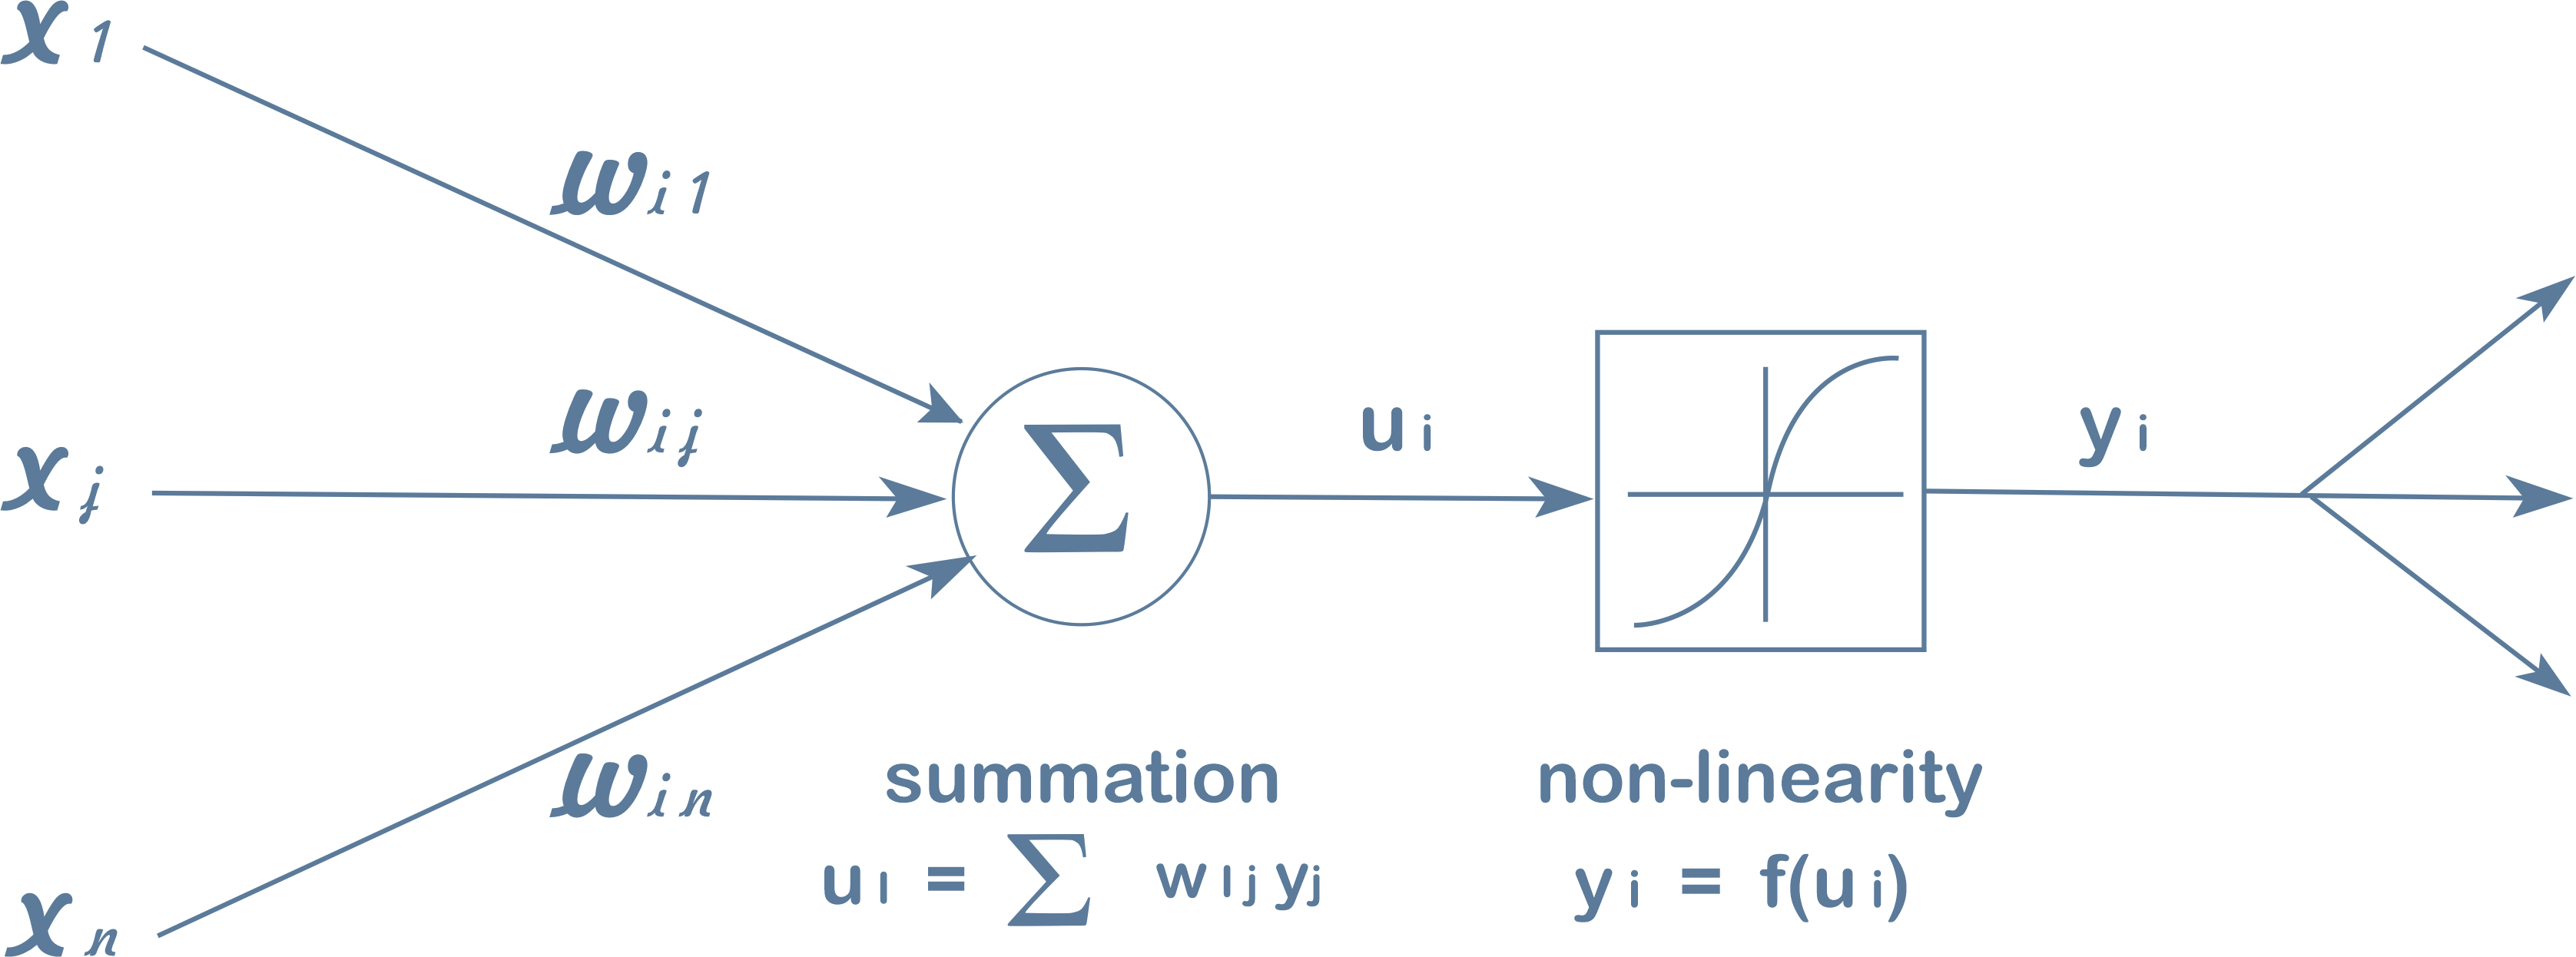
\includegraphics[width=0.8\textwidth]{images/comparacion_neuronas.jpg}
\centering
\caption{Comparacion entre una neurona real y una artificial \cite{neuronas}.}
\label{neurona}
\end{figure}

Una MLP consta de varias capas ``densas'' de neuronas conectadas entre ellas. Una vez 
realizado el procesamiento de las entradas por toda la red neuronal, comienza el 
proceso de modificación de los pesos \textit{w} de cada una de las capas. Este proceso 
se llama ``retro propagación'' o \textit{back propagation} y consiste en propagar las 
derivadas de cada una de las funciones de las neuronas desde la última capa hasta 
la primera.\\

Este modelo espera como entrada un vector de datos lineales. Es por ello que este tipo 
de modelos no es especialmente bueno para poder extraer la información de las imágenes 
ya que realizar este proceso sería demasiado complejo computacionalmente hablando. 
En caso contrario, se podría utilizar un extractor de características para mejorar la 
eficiencia. Lamentablemente esto ocasionaría una pérdida de datos, y, por último, 
que la información de una imagen suele cumplir el principio de localidad (la información 
relevante suele estar reunida en espacios cercanos) y vectorizarla estaría omitiendo 
características importantes para su análisis.

\subsection{\textit{Convolutional Neural Networks} (CNN)}

Las CNN's son modelos basados en una arquitectura especialmente diseñada para el 
análisis de imágenes y en especial, su clasificación. Ellas realizan la labor de 
extracción de características que no realiza el MLP a través de convoluciones. Esto 
evita la perdida de información y mejoran su eficiencia y precisión sobre todo. \\

Las convoluciones se basan en un procedimiento que permite extraer características al 
aplicar una matriz cuadrada de transformación (generalmente bastante pequeña) a lo 
largo de la imagen original, la cual luego devuelve otra imagen modificada. Estas 
matrices de transformación son llamadas kernels. En la figura \ref{convolucion} se 
ilustra una iteración de la convolución.
\\
\begin{figure}[h!]
\includegraphics[width=0.7\textwidth]{images/convolución.png}
\centering
\caption{Proceso de convolución simplificado\cite{convoluciones}.}
\label{convolucion}
\end{figure}

Por otra parte, existen otras capas importantes, los \textit{poolings}, como se ilustra 
en la imagen \ref{pooling}. Estas capas consisten de la aplicación de una lógica a un 
cuadrante de la matriz resultante de las convoluciones. Esta lógica varía dependiendo 
de las necesidades del usuario. En la imagen mencionada anteriormente se puede ver la 
comparación entre el \textit{Max Pooling} y el \textit{Average Pooling}, las cuales 
obtienen el máximo y el promedio de los cuadrantes seleccionados para generar un nuevo 
resultado de menor dimensión. 

\begin{figure}[h!]
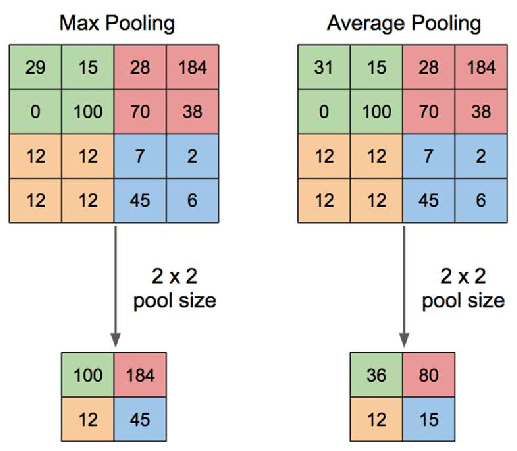
\includegraphics[width=0.6\textwidth]{images/pooling.png}
\centering
\caption{Proceso de convolución simplificado \cite{pooling}.}
\label{pooling}
\end{figure}

Las CNN's se conforman por la unión de capas convolucionales y \textit{pooling} repetidas 
veces, terminando en una MLP, la cual realiza el trabajo final del procesamiento de las 
características extraídas. En la imagen \ref{CNN} se puede ver la estructura de una CNN. 
Como se mencionó anteriormente, el proceso de la extracción de características se realiza 
dentro de la misma red neuronal, evitando perdida de información a comparación de la MLP, 
dejándole a esta unicamente el trabajo de la clasificación.

\begin{figure}[h!]
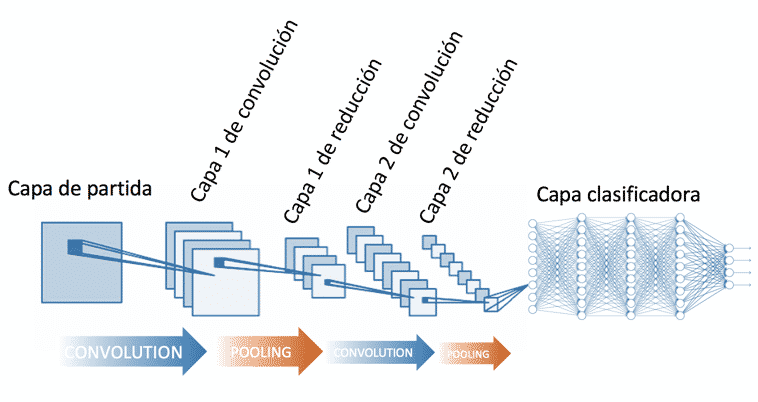
\includegraphics[width=1\textwidth]{images/CNN.png}
\centering
\caption {Arquitectura general de una CNN\cite{CNN-Arquitectura}. }
\label{CNN}
\end{figure}



\section{Arquitecturas del estado del arte}
\label{arquitecturas}

\subsection{VGG-19}
Esta CNN tiene 19 capas de profundidad y fue creada por Karen Simonyan y Andrew Zisserman 
\cite{Simonyan2015} en la Universidad de Oxford en 2014, y posteriormente publicado en 
2015. Su versión detallada se ilustra en la imagen \ref{VGG19}. Este modelo fue utilizado 
para intentar clasificar las imagenes del 
\textit{dataset} ImageNet, llegando a clasificar hasta 1000 objetos diferentes. 
Este modelo espera una imagen de 224x224 píxeles como entrada para su procesamiento. 
Debido a su profundidad, este modelo es bastante pesado, llegando a consumir 550 MB de 
memoria con alrededor de 143 millones de características. Cabe resaltar que el 70\% de 
todas estas características se encuentran en el paso entre la última capa convolucional y la 
primera de clasificación. Con todas estas características, logró obtener un resultado 
de 90\% de precisión con ImageNet.

\begin{figure}[h!]
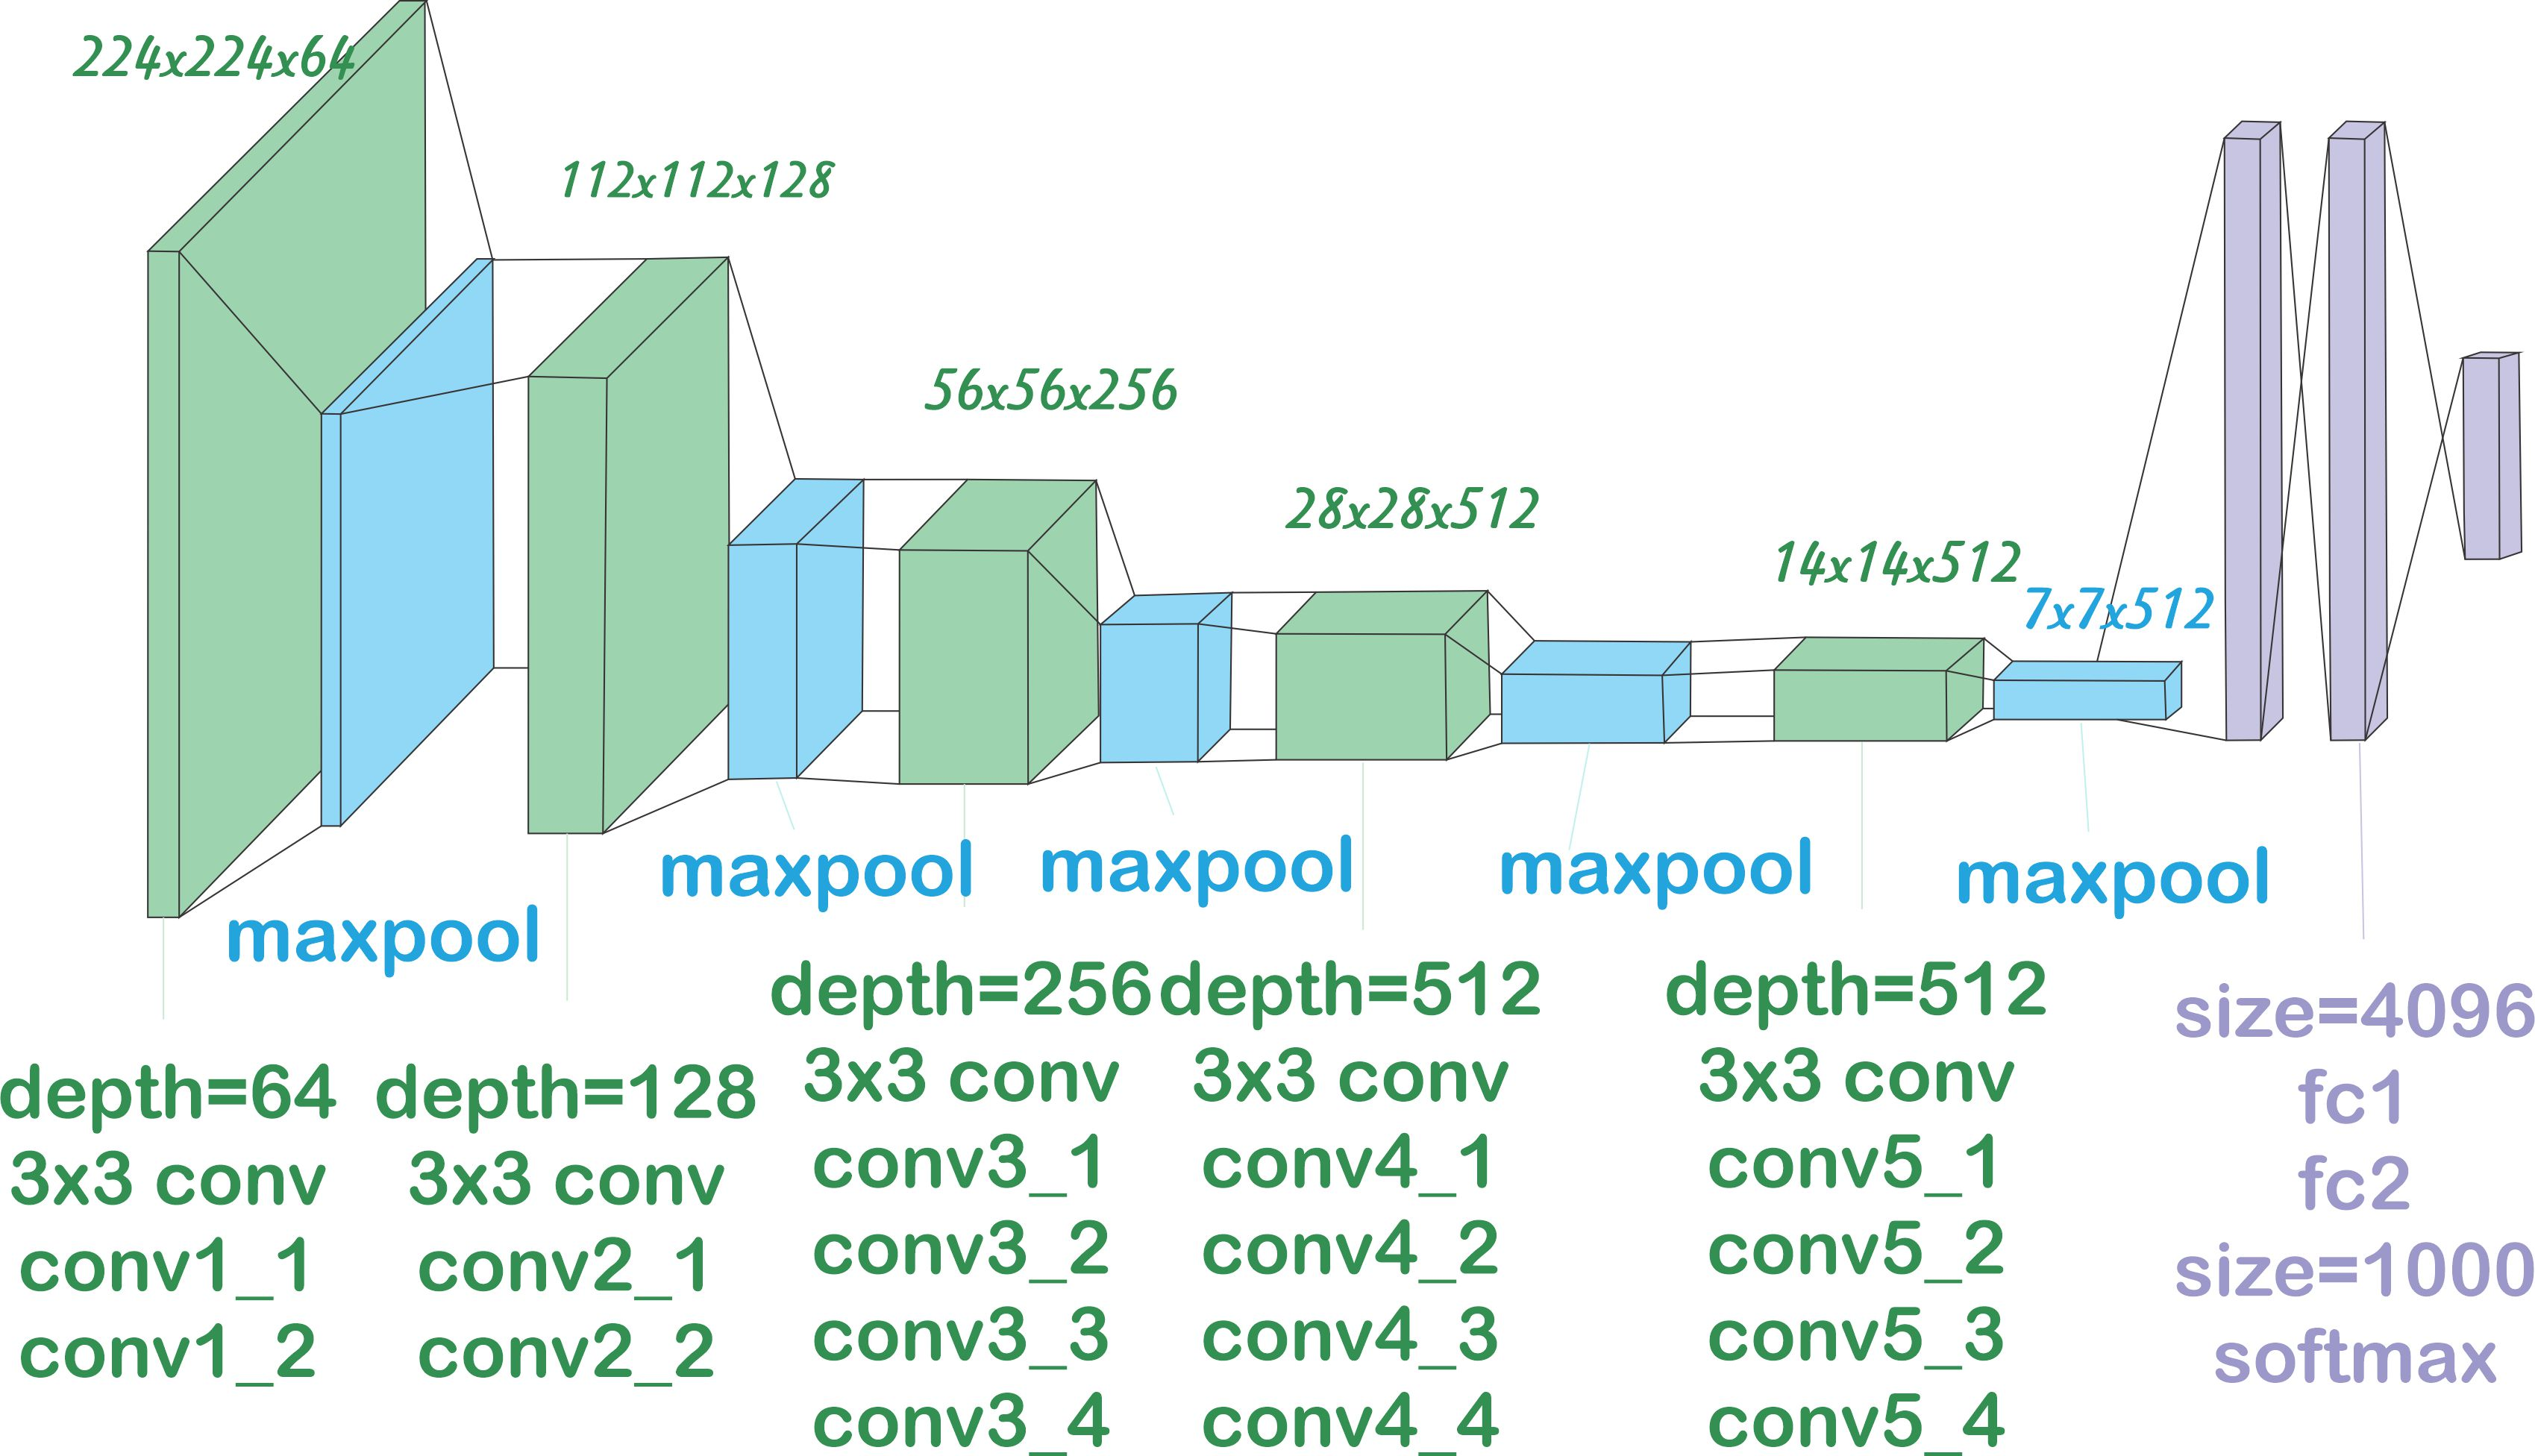
\includegraphics[width=1\textwidth]{images/VGG19.jpeg}
\centering
\caption{Versión simplificada de VGG19 \cite{modelos}. }
\label{VGG19}
\end{figure}

\subsection{InceptionV3}
\label{sec:inceptionV3}

Si bien VGG19 lograba obtener una precisión muy elevada, esta consumía demasiados 
recursos. Es por ello que Google desarrolló InceptionV3, una red que prometió obtener los 
mismos resultados pero con menor costo. Presentado en ``\textit{Going deeper with convolutions}'' 
\cite{Szegedy2014}, este modelo alcanza una precisión del 93.7\% con el mismo \textit{dataset}. 
\\
Si bien esta red contiene 50 capas de profundidad (las cuales superan a las de la VGG19), el 
número de características a entrenar era menor (23.8 millones). Su propuesta planteaba que
realizar convoluciones unidimensionales en serie (como se ve en la figura \ref{InceptionLayer}), 
equivale a realizar una convolución bidimensional, evitando el uso de filtros matriciales. 
En ese sentido disminuyeron la complejidad que se tenía en los modelos de CNN convencionales, 
haciéndolo mas ligero en memoria y aumentando la capacidad de aprendizaje del modelo. En total, 
este modelo llega a pesar 92 MB, lo cual es alrededor de 6 veces menor que el anterior. Su 
entrada requiere de imágenes de 299x299 píxeles y su arquitectura se ve reflejada en la figura 
\ref{Inceptionv3}.

\begin{figure}[h!]
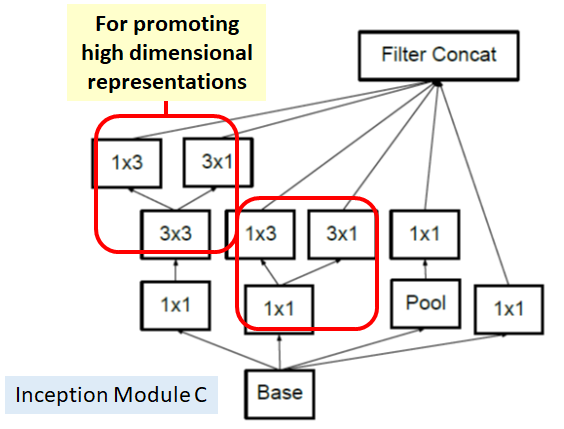
\includegraphics[width=0.8\textwidth]{images/InceptionLayer.png}
\centering
\caption{Reducción de la dimensionalidad del InceptionV3. \cite{modelos} }
\label{InceptionLayer}
\end{figure}

\begin{figure}[h!]
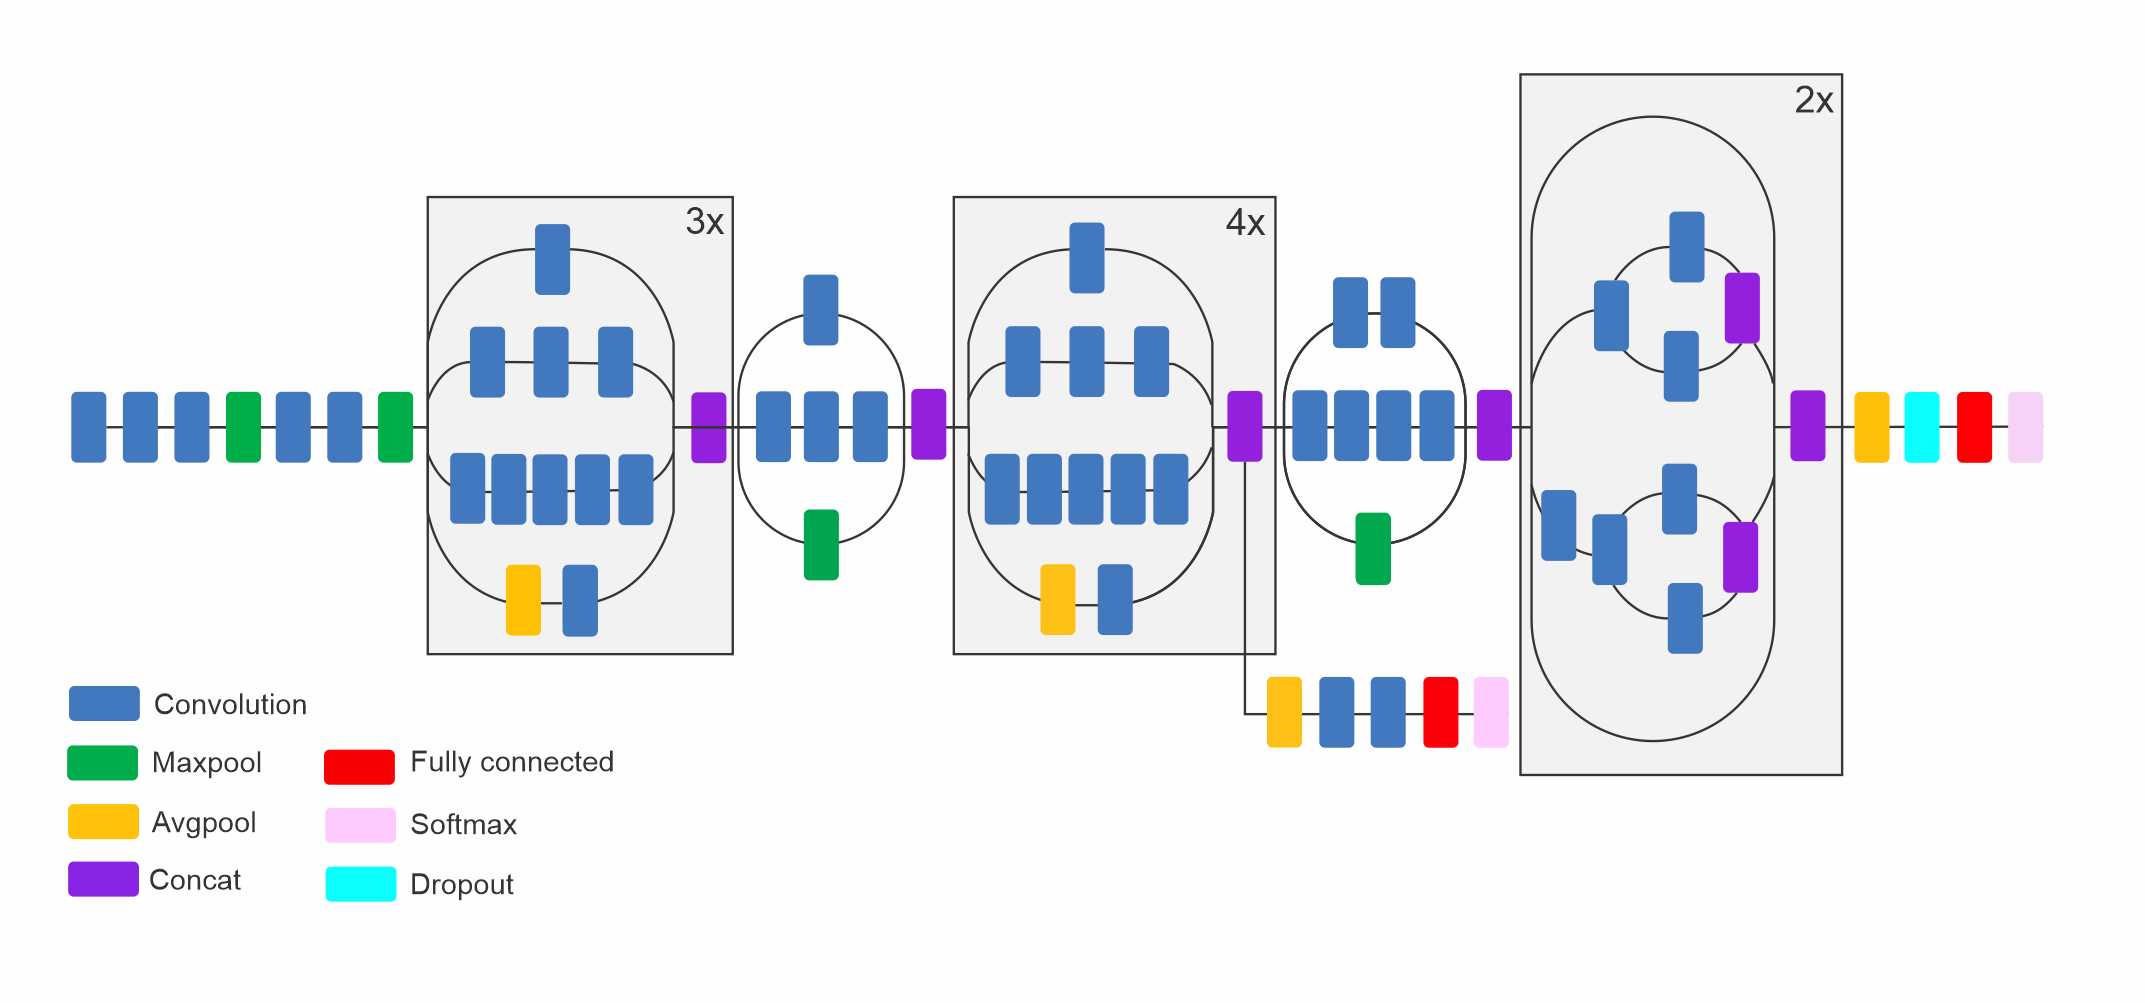
\includegraphics[width=1\textwidth]{images/InceptionV3.png}
\centering
\caption{Versión simplificada de InceptionV3. \cite{modelos} }
\label{Inceptionv3}
\end{figure}

\subsection{ResNet50}
Creada por Microsoft en 2015, cuenta también con 50 capas profundas. Este modelo emplea 
una técnica llamada ``aprendizaje residual'' \cite{He2015}, la cual consiste en guardar una 
copia de lo aprendido actualmente, y sumarlo al resultado obtenido de aplicar una cantidad de 
convoluciones (en este caso cada tres). La imagen \ref{ResNet} ilustra esta modificación dentro 
del modelo además de su arquitectura general. Este modelo también fue probado con el mismo 
\textit{dataset}, obteniendo un 92.1\% de precisión y gracias al aprendizaje residual se evito 
aumentar la dimensionalidad del modelo. Esta red contiene aproximadamente 25.6 millones de 
características y ocupa 98MB de memoria. 

\begin{figure}[h!]
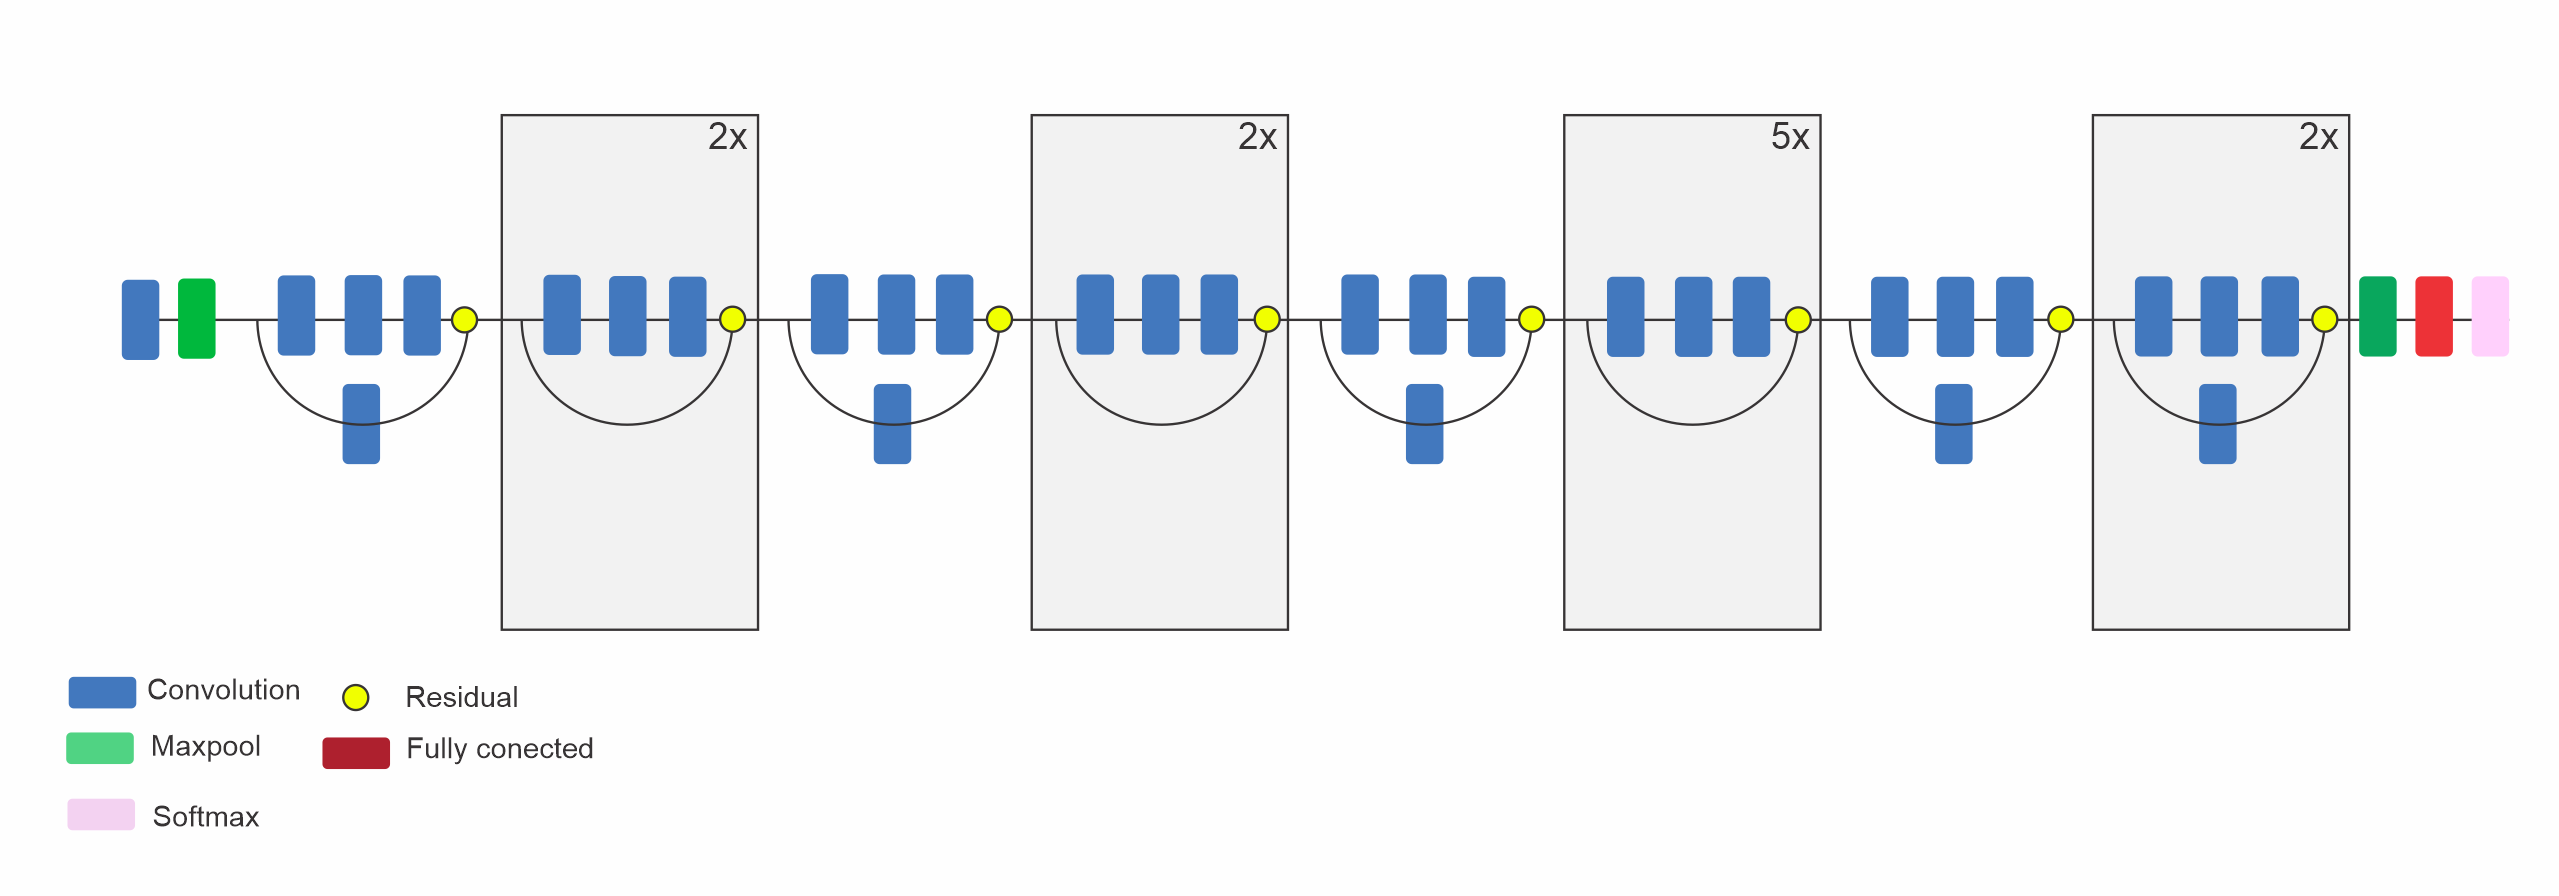
\includegraphics[width=1\textwidth]{images/ResNet.png}
\centering
\caption{Versión simplificada de ResNet50. \cite{modelos} }
\label{ResNet}
\end{figure}


\subsection{EfficientNet}

Creada por Google en 2019 y publicada en ``\textit{EfficientNet: Rethinking Model 
Scaling for Convolutional Neural Networks}'' \cite{Tan2020} en 2020, consta de 8 
implementaciones diferentes (B0 a B7). La implementación más liviana (B0) consiste 
de aproximadamente 5.5 millones de características, siendo probada en el mismo 
\textit{dataset} con una precisión de 93\%. Las demás implementaciones continúan 
aumentando el número de características y a su vez la precisión que obtienen. Haciendo 
una comparación con los anteriores modelos, EfficientNetB4, el cual consta de 19.5 
millones de características, genera una precisión de 96.4\%, superándolos. La manera 
en la que este modelo optimiza su propio aprendizaje es a través de un algoritmo de 
aproximación que permite generar parámetros para la creación de cada uno de los ocho 
modelos. Este algoritmo toma en cuenta 3 factores:

\begin{itemize}
    \item Profundidad de las capas
    \item Ancho de las capas (multicapa)
    \item Resolución de las imágenes
\end{itemize}
En la figura \ref{EfficientNetB0} se puede ver la estructura de la EfficientNetB0. 


\begin{figure}[h!]
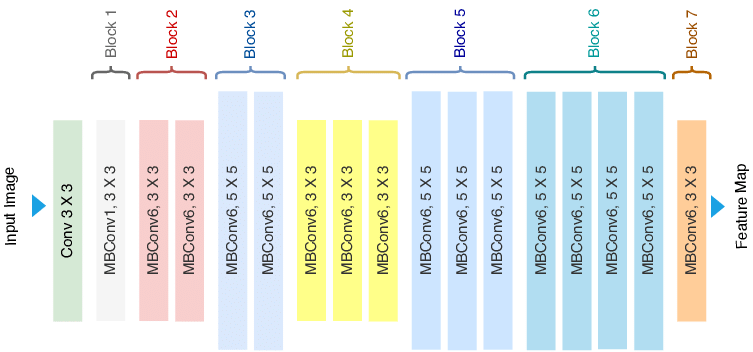
\includegraphics[width=1\textwidth]{images/EfficientNetB0.png}
\centering
\caption{Versión simplificada de EfficientNetB0. \cite{EfficientNetB0} }
\label{EfficientNetB0}
\end{figure}

\subsection{YOLO}
YOLO (\textit{you only look once}) se presenta como una arquitectura que permite 
``predecir simultáneamente múltiples cuadros delimitadores (\textit{bounding boxes}) 
y probabilidades de su clase para ellos'' \cite{Redmon2015}. Este modelo se basa en 
una CNN convencional, la cual a comparación de implementaciones previas (R-CNN y FR-CNN) 
realiza la predicción de los \textit{bounding boxes} de manera interna, permitiendo una 
menor latencia, creando un modelo factible para su uso en tiempo real.\\

Este cálculo se realiza en base a la generación de grillas (\textit{grids}) o secciones 
de la imagen, dentro de las cuales se inicializan un número de \textit{bounding boxes} 
predeterminados, ambos siendo hiperparámetros de la arquitectura. Esta es replicable 
utilizando cualquier arquitectura de CNN como base, como por ejemplo alguna de las 
anteriormente mencionadas, solamente ajustando la salida e hiperparámetros correspondientes. 
Versiones más modernas obtienen una mejor capacidad de detección, módulos de atención, 
entre otras variaciones que lo hacen cada vez más robusto. En la imagen \ref{YOLO} se 
puede ver ejemplificada la arquitectura del modelo yolov5.

\begin{figure}[h!]
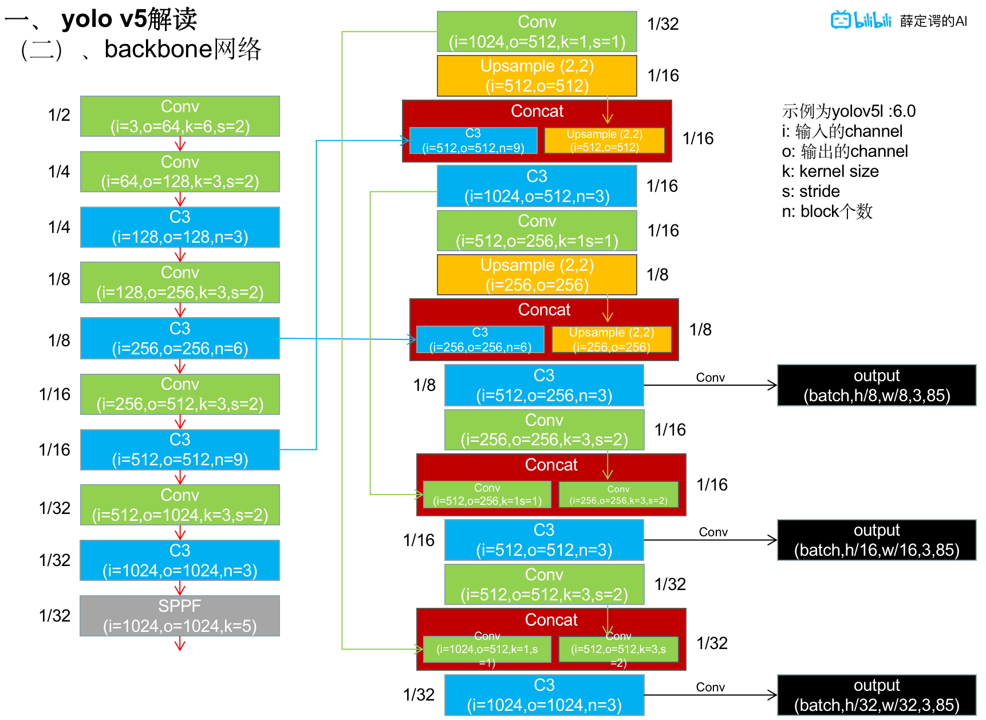
\includegraphics[width=1\textwidth]{images/yolov5.png}
\centering
\caption{Representación de la arquitectura YOLOV5 \cite{yolov5}}
\label{YOLO}
\end{figure}

\subsection{UniDet}

\textit{Unified Detector} (UniDet) fue presentado en el año 2022 e intenta resolver 
el problema de la unificación de \textit{datasets} para la creación de un modelo 
robusto que logre también predecir en \textit{datasets} externos a los de entrenamiento, 
generando una precisión comparable al estado del arte. Esta arquitectura consta de un 
\textit{backbone} (extractor de características), que pasa después a tres diferentes 
\textit{heads} (quien realiza la detección y clasifica el \textit{bounding box} por cada 
dataset para luego finalmente generar una respuesta unificada. Esta arquitectura se puede 
resumir en la imagen \ref{fig:unidet}

\begin{figure}[h!]
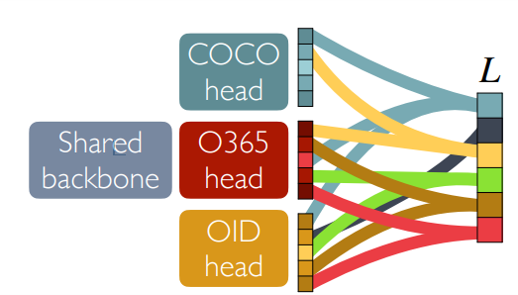
\includegraphics[width=1\textwidth]{images/imagenUnidet.png}
\centering
\caption{Representación de la arquitectura UniDet \cite{unidet}.}
\label{fig:unidet}
\end{figure}

El \textit{backbone} esta basado en una arquitectura Cascade RCNN, el cuál consiste de usos recursivos de capas convolucionales, \textit{heads} y generación de predicciones para manejar imágenes borrosas utilizando una técnica de \textit{resampling} a través de la recursividad mencionada. La arquitectura de este modelo está resumida en la imagen \ref{fig:cascade}

\begin{figure}[h!]
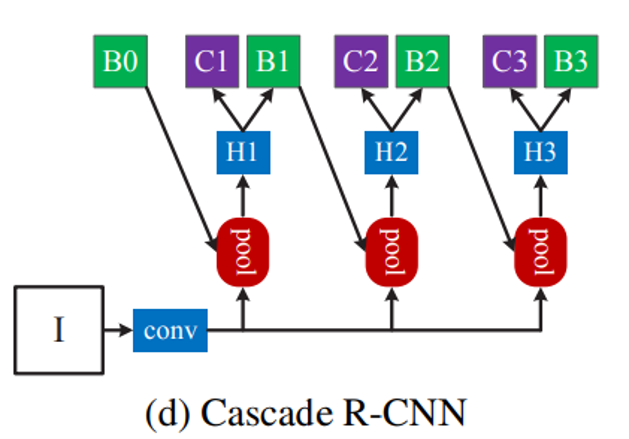
\includegraphics[width=0.6\textwidth]{images/cascadercnn.png}
\centering
\caption{Representación de la arquitectura Cascade RCNN \cite{cascadercnn}.}
\label{fig:cascade}
\end{figure}

Esta arquitectura representa el estado del arte en el tema de detección y clasificación en la 
mayoría de los \textit{datasets} más comunes tales como COCO, Objects365, Open Images, VOC, 
VIPER, entre otros.  

\section{\textit{Transfer Learning}}
Según Muhamad Yani \cite{Yani2019}, se le llama \textit{Transfer Learning(TL)} al ``proceso de  
transferencia del conocimiento de un entrenamiento previo para ser usado en un nuevo modelo para la 
reducción de tiempo en el proceso de aprendizaje''. En la figura \ref{transfer-learning} se 
puede evidenciar este proceso.\\ 

\begin{figure}[h!]
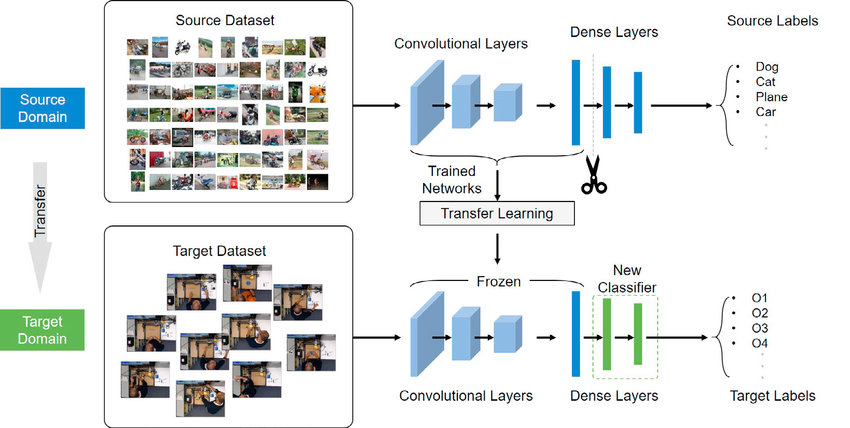
\includegraphics[width=1\textwidth]{images/transfer-learning.png}
\centering
\caption{Comparación entre el aprendizaje común y transfer learning. \cite{transfer-learning}}
\label{transfer-learning}
\end{figure}

TL difiere del proceso convencional de entrenamiento de una red ya que no es necesario 
entrenarlo con un \textit{dataset} grande. En contraste con el proceso convencional, se congelan las 
capas iniciales del modelo (en nuestro caso las capas convolucionales), las cuales tienen todo el 
conocimiento pre-aprendido por la red sobre el \textit{dataset} con el que fue diseñado. Una vez 
obtenidas esas capas, se les anexan nuevas capas densas (iguales a las de un MLP) para servir como 
los clasificadores para nuestro uso. Gracias a esto, únicamente es necesario entrenar las capas finales, 
lo cual no necesita tantos datos y generando predicciones generalmente certeras. A este tipo de 
entrenamiento se le llama ``\textit{fine tuning}'' o ajuste, que permite a la red modificar el aprendizaje 
anterior para poder predecir en base a un \textit{dataset} diferente al que fue originalmente entrenado, 
ahorrando tiempo y mejorando su precisión.

\section{Pre-procesamiento de Entradas}
Teniendo conocimientos generales acerca de cómo funcionan estos modelos, necesitamos ahora conocer acerca 
de las características necesarias de las entradas para que el modelo aprenda.

\subsection{Tamaño de entrada}
Tomando únicamente en cuenta a las diferentes CNN, cada uno de los modelos espera una matriz (la imagen) de diferente tamaño. En las implementaciones actuales, se suele utilizar tensores para referenciar un \textit{batch} (conjunto) de imágenes. La representación es la siguiente:
$$(batch,canales, m,n), donde:$$
\begin{itemize}
    \item batch: Numero de imagenes que se estan ingresando a la vez
    \item canales: Numero de canales de la imagen (en caso de ser a color, serian 3 canales representando RGB, mientras que a blanco y negro sería solo 1 canal)
    \item m \& n: dimensiones de la imagen. Estos datos dependen de la arquitectura del modelo ya 
    que cada capa realizará operaciones que irán disminuyendo la dimensionalidad 
    de la misma. Esto varía con cada implementación debido a las diferentes configuraciones 
    que se pueden hacer a cada matriz convolucional y a los \textit{pooling}.
\end{itemize}

\subsection {\textit{One Hot Encoder}}
Este es un tipo de representación que consiste en la creación de una matriz de identidad 
de tamaño \$n x \$n, donde \$n es el numero de \textit{labels}. La codificación de cada uno de 
los labels se puede tomar como una de las filas de la matriz. En ese sentido podemos 
representar la codificación de un objeto de la clase j, de n clases como:

$$OneHotEncoder(i,j,n)= [a_1,a_2, .. a_n], donde: $$
\begin{equation*}
a_{i,j}=
\begin{cases}
1 & \text{j = i}\\
0 &  \text{Caso contrario}
\end{cases}
\end{equation*}

Este tipo de codificación trae como ventaja el hecho de que se evita la necesidad 
de tener una relación entre los labels, además de permitir obtener una clasificación 
directa a la hora de comparar los resultados. Por contraparte, tiene como desventaja 
la alta dimensionalidad si se tienen muchos \textit{labels}.



\section{\textit{Overfitting}}
El proceso por el cual los modelos aprenden es gracias a la retroalimentación que se obtiene realizando la retroprogacación mencionada anteriormente. Una vez actualizados los pesos de cada neurona con la gradiente que se obtiene, se podría afirmar que el modelo ya logró aprender a clasificar esa imagen especifica. Sin embargo, esta gradiente se puede desvanecer debido a la profundidad de la arquitectura, las funciones de activación, entre otros motivos. Este desvanecimiento de la gradiente evita que el modelo continue aprendiendo del \textit{dataset}, haciendo al modelo inservible para usos reales. Algunas de las estrategias aplicadas son: 

\begin{itemize}
    \item {\textit{Data Augmentation}: Aumentar el \textit{dataset} original en base a rotaciones, escalados, cortados, simetría, etc. Con ello el entrenamiento del modelo se hace más resistente a estos cambios en la posición o rotación del objeto en la imagen }
    \item {\textit{Batch Normalization}: Re-escalar los datos de entrada a en diferentes escalas respecto a una escala común para poder generar una distribución de los datos más manegable.}
    \item {\textit{Dropout}: Desactivar de manera aleatoria un porcentaje de las neuronas artificiales de una capa. Esto obliga a cada neurona a no depender de las neuronas desactivada, generando una mejora en general.}
\end{itemize}

En el presente capítulo se presentaron conocimientos previos que servirán al lector a entender un poco más acerca de la metodología que en el futuro se va a presentar, en especial las arquitecturas de los modelos que se planea revisar, utilizar y comparar para poder obtener el mejor resultado posible para la detección y clasificación de imágenes de peces dentro de la fauna marina peruana. 



\chapter{REVISI\'ON DE LA LITERATURA}

En el presente capítulo se analizarán los modelos y técnicas de DL 
para la clasificación de imágenes y su impacto en algunas aplicaciones 
actuales. Como ya había sido mencionado, los modelos de DL son los que 
en la actualidad han reemplazado a varios algoritmos y al humano mismo 
en las diferentes tareas de regresión, clasificación, detección y 
localización de objetos en imágenes. Esto gracias a su gran precisión 
en esta tarea y a la automatización que traen a las diferentes empresas 
e instituciones gubernamentales. \\

Alsmadi y Almarashdeh \cite{Alsmadi2022} lo comprobaron al realizar un 
\textit{survey} donde revisaban y comparaban trabajos con diferentes 
enfoques. En la investigación compararon algoritmos de visión 
computacional, estadística, ML, DL, entre otros, aplicados al contexto de 
extracción de características, detección y clasificación. Corroboraron 
que la eficacia y velocidad de los modelos de DL fueron superiores 
a los demás algoritmos clásicos.\\

Dentro del sub-área de DL, Xiaojuan Lan, \textit{et al}.\cite{10.1145/3419635.3419643} 
son los autores revisados mas recientes. Ellos diseñaron un modelo utilizando TL en 
base a Inception-V3,(ver sección \hyperref[sec:inceptionV3]{2.2.2}), para resolver el 
problema de la clasificación de imágenes borrosas de peces en el fondo marino con una 
precisión de más del 85\% y de manera más eficiente que otros modelos pre-existentes. 
Un punto que cabe resaltar de este trabajo es que detallan que utilizaron 
InceptionV3 como base para el TL, pero no mencionan qué capas del modelo se congelaron y 
cuales fueron cambiadas para su adaptación a su \textit{dataset} sino que saltan directamente 
a las conclusiones, dando como resultado la precisión promedio, lo cual podría esconder 
que ellos obtuviesen un modelo \textit{overfitted}, considerando también la baja cantidad 
de imágenes de su \textit{dataset}. \\

De la misma manera, Nibha Manandhar y John W. Burris \cite{10.1145/3325917.3325934}, 
quienes utilizaron las mismas herramientas mencionadas anteriormente, pero enfocándose a 
una problemática diferente. En vez de predecir si la imagen era de un determinado tipo de 
pez, predecían si ``la imagen contenía esa determinada especie de pez dentro'', ya 
que no eran imágenes del hábitat de los peces sino imágenes recuperadas de Google, que 
podían contener seres humanos u otro entorno y no únicamente el pez. Con este enfoque lograron 
obtener una precisión del 85\% en la etapa de entrenamiento. \\


De la misma manera que en el trabajo de Xiaojuan Lan, \textit{et al}, no especifican a detalle 
como es que se está realizando el TL en el modelo. Además, en la sección de resultados 
muestran que se generó una buena precisión solo en algunas especies, mientras que en otras 
alcanzó alrededor de 50 a 70\% \\

Por último, Guang Chen, \textit{et al}. \cite{8371919} realizaron un modelo en base a 2 ramas, 
una para la clasificación a nivel de imagen y la otra para la clasificación a nivel de instancia 
de las imágenes. Mientras que la primera se basaba únicamente en un modelo sencillo de CNN, la 
segunda se basaba en un proceso de cuatro pasos:
\begin{itemize}
    \item Detección: Utilizó los modelos YOLOv2 y SSD, realizando el cálculo de los \textit{bounding boxes}, los cuales contienen coordenadas de las dos esquinas del rectángulo que contiene al pez.
    \item Estimación de la pose: Se maneja otro modelo de CNN para definir la dirección del pez como un problema de clasificación (se está clasificando la dirección hacia donde apunta la cabeza del pez).
    \item Alineamiento: Se rota la imagen para que el pez mantenga una dirección horizontal y mirando hacia la derecha.
    \item Predicción: Se aplica otro modelo de CNN para la clasificación de la imagen obtenida.
\end{itemize}
Hay varios aspectos positivos en este trabajo. El primero es que nos da detalle acerca de todo 
el procedimiento que se necesitó para realizar la implementación de su modelo. Segundo, combinan 
muchas técnicas y modelos para hacer más robusta su propuesta. Por último, obtuvieron un resultado 
que no solo clasificaba al pez como tal, sino que utilizaba características del entorno y de los 
objetos cercanos para poder hacer su labor de clasificación. \\

Por otra parte, considero que la estimación de la pose y el alineamiento son pasos que no eran 
necesarios en este \textit{pipeline} ya que las CNN's del estado del arte suelen ser resistentes 
a este tipo de problemas. Esto podría haber tenido influencia en el costo computacional del mismo, 
haciéndolo más lento y podría haber tenido una mejor precisión sin ello. \\

Dentro de la problemática de localización de fauna marina, Suxia Cui, \textit{et al}. \cite{Cui2020} 
desarrollaron un modelo para localizar y clasificar los peces dentro del agua a través de un 
\textit{Autonomous Underwater Vehicle (AUV)}. El modelo consistió en 24 capas convolusionales, a las 
cuales les siguen dos capas \textit{full conected}. Ellos se inspiraron en la arquitectura del modelo 
YOLO para poder realizar la localización de los peces.\\

Al igual que el trabajo anterior, uno de los puntos mas favorables de este es que documenta tanto el 
procedimiento como los métodos utilizados, además de evidenciar unos buenos resultados para la localización 
y clasificación de múltiples peces dentro de una imagen dentro del océano, el cual ya es de por sí un gran 
desafío. Un problema que suele ocurrir con este tipo de modelos es la falta de imágenes etiquetada para el 
entrenamiento de los modelos, haciendo inviable la creación de este tipo de modelos en casos reales.\\

Dentro del área de Visión Computacional (VC) se encuentra el trabajo de Mejía y Rosales 
\cite{20.500.12724/11174}, quienes son los únicos autores que han investigado sobre el uso 
de técnicas de DL para la clasificación de la fauna marina peruana por el momento. Ellos se 
basaron en el documento de Suxia Cui,\textit{et al}. para su trabajo. Si bien desarrollaron como 
solución final un modelo de DL para la clasificación, este era retro-alimentado a través de 
varios algoritmos de visión computacional.\\

Entre estos algoritmos de visión se encuentran los algoritmos SURF/SIFT, el cual se encarga de obtener la 
silueta de un pez utilizando diferencias gaussianas de la posición-escala de cada pixel. Una vez obtenida 
la silueta, se procede eliminar el \textit{background} y se identifican los bordes del pez, siendo este 
resultado analizado y después usado para el entrenamiento del modelo. Con este, lograron obtener un 80\% 
de precisión en la etapa de testeo.\\

El mayor aporte de este trabajo ha sido la experimentación de nuevas entradas para las CNN's a través de un 
pre-procesamiento, queriendo mejorar la precisión del modelo final. Aún así, pareciera que el valor de precisión 
obtenido podría tener un \textit{overfit} debido a que no muestra ejemplos de las imágenes utilizadas, el número de 
ellas y a la alta precisión final. Por otra parte, las CNN's fueron diseñadas para que las imágenes sean pasadas 
enteramente como entradas sin tener ese procesamiento inicial.\\

Como se pudo ver a lo largo de este capítulo, los algoritmos de detección y clasificación de 
imágenes han ido evolucionando, lo cual llevó a diferentes investigadores a utilizar algoritmos de ML y DL para estas tareas. En el 
presente capítulo se presentaron algunas de las investigaciones del estado del arte enfocadas en modelos de CNN y 
YOLO para la detección y clasificación de imágenes en diferentes \textit{datasets}. Dentro de ellas, se pudo ver 
diferentes \textit{pipelines} que lograron obtener una precisión muy elevada para problemas complejos, por lo cual el 
presente trabajo planea seguir con esa línea de investigación y proponer un nuevo \textit{pipeline} para mejorar la detección y 
clasificación de peces dentro de la fauna marina peruana.   

\chapter{METODOLOG\'IA}

En este capítulo, se describe la metodología planificada para emplearse en 
las experimentaciones detalladas en capítulos subsiguientes. La Figura \ref{pipeline} 
muestra el pipeline propuesto para la ejecución de estos experimentos.  \\

\begin{figure}[h!]
\includegraphics[width=0.85\textwidth]{images/Metodología.png}
\centering
\caption{Pipeline propuesto.  }
\label{pipeline}
\end{figure}

\section{\textit{Dataset}}

Para cada tipo de aplicación de ML, se tienen diferentes conjuntos de datos 
disponibles. Sin embargo, entre ellos es importante destacar que existen 
distintos tipos y se puede observar que algunos son más o menos 
complejos para ciertas tareas dependiendo del tamaño, número y la 
calidad de los datos.
\\

En el caso de la tarea de detección y clasificación de imágenes, 
se considera un \textit{dataset} de baja complejidad como aquel 
que contiene imágenes con objetos centrados, alineados en una sola 
dirección, con una resolución óptima y enfocados en el centro. Se ha 
demostrado en el marco teórico y en la revisión del estado del arte que 
este tipo de conjuntos de datos son fáciles de clasificar, 
especialmente para modelos como los mencionados en la sección \ref{arquitecturas}.
\\

En contraste, un conjunto de datos complejo difiere considerablemente de 
esta descripción. Las imágenes pueden contener varios objetos que no son 
los que se deben clasificar, presentando desalineación, baja resolución 
o falta de enfoque. Estas características dificultan que las redes 
neuronales convolucionales (CNN) logren una alta precisión, ya que no 
pueden aprender todos los patrones y realizar predicciones precisas para 
cada objeto. La Figura \ref{fig:combined} ilustra claramente la marcada 
diferencia entre estos dos tipos de conjuntos de datos.
\\

\begin{figure}
    \centering
    \subfloat[\centering Imagen de un \textit{dataset} ``poco complejo'' obtenido de \href{https://www.kaggle.com/datasets/giannisgeorgiou/fish-species}{\textit{Fish Species}}]{{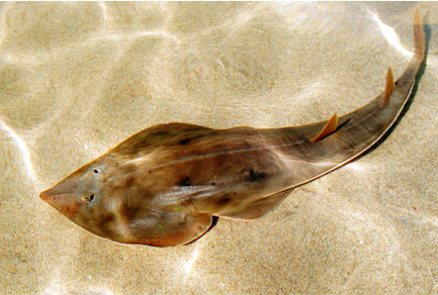
\includegraphics[width=4cm]{images/pezGuitarra.png} }}%
    \qquad
    \subfloat[\centering Imagen de un \textit{dataset} ``complejo'' obtenido de \href{https://www.kaggle.com/c/the-nature-conservancy-fisheries-monitoring}{\textit{The Nature Conservancy}}]{{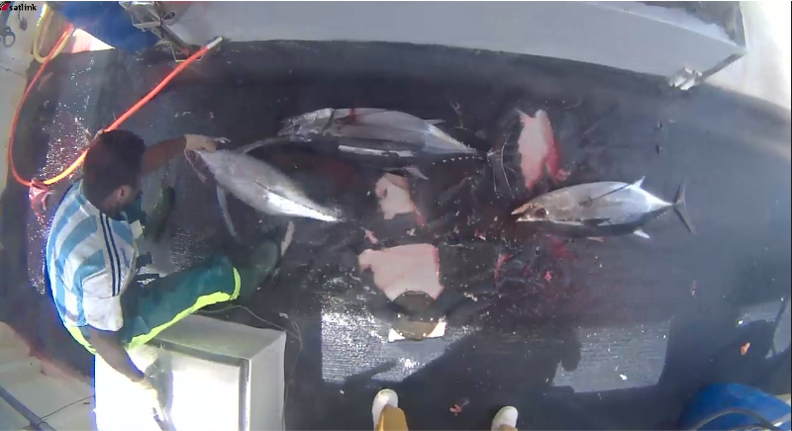
\includegraphics[width=5cm]{images/Bet.png} }}%
    \caption{Comparación de imágenes dentro de datasets diferentes}%
    \label{fig:combined}
\end{figure}
Además, los \textit{datasets} según su función de distribución de imágenes y 
el objetivo específico recaen en dos categorías. En la primera categoría, 
encontramos conjuntos de datos homogéneos y heterogéneos. Los \textit{datasets} 
homogéneos se caracterizan por 
tener la misma cantidad (o un número similar) de muestras por clase, lo que 
permite que los modelos aprendan de manera equitativa de cada clase. Sin embargo, 
esto no siempre refleja la realidad, donde la probabilidad de que aparezca una 
clase de objeto determinada puede ser mayor o menor que otra.
\\

En ese sentido, los \textit{heterogéneos} son aquellos que no tienen un 
número igual de muestras para cada clase. Esto puede ser intencional, ya que el 
creador del conjunto de datos diseñó la distribución de muestras de esa manera, o 
puede ser resultado de la falta de muestras disponibles.
\\

Además, los \textit{datasets} suelen venir etiquetados en relación a su objetivo. 
En nuestro caso, para entrenar una CNN, se dispone de un repositorio de imágenes 
junto, cada una dentro de una carpeta con el nombre de su respectiva clase. En 
cambio, para entrenar una red como YOLO, se requieren los ``bounding boxes'' que 
delimitan la ubicación de los objetos.
\\

Dado que encontrar un \textit{dataset} de imágenes etiquetadas de peces resulta 
inviable para el caso peruano, se han utilizado dos tipos de conjuntos de datos 
encontrados en la plataforma Kaggle para esta investigación. Ambos conjuntos contienen 
imágenes y sus respectivas etiquetas, pero uno presenta peces centrados y sin ruido, 
mientras que el otro incluye fotografías tomadas en un entorno real donde se encuentran 
peces, personas e instrumentos de pesca, lo que lo convierte en un conjunto de datos 
heterogéneo. El primero se utilizará para realizar comparaciones entre los modelos, 
mientras que el segundo se empleará para el entrenamiento y prueba del pipeline final.
\\

Estas imágenes fueron re-dimensionadas dependiendo del tamaño de entrada que se espera 
para cada red, y luego fueron pasadas al clasificador.

\section{Detector}
Para la detección de cada imagen del \textit{dataset}, se utilizó un módulo de detección 
basado en YOLO v5, el cual ya ha sido preentrenado con el conjunto de datos ``Objects365'', 
brindando la capacidad de detectar la categoría de peces. Además, se entrenó un YOLO v5 con 
el \textit{dataset}, ignorando las clases detectadas. Por último, también utilizaremos un 
modelo llamado UniDet, el cual ha sido entrenado con los \textit{datasets} ``Objects365'', 
``OpenImages'' y ``COCO''.  Una vez que las imágenes sean procesadas por el detector, 
esperamos obtener \textit{los bounding boxes} donde se encuentren los peces individualmente. 
Se puede visualizar este proceso en la figura \ref{fig:detector_pez}.
\begin{figure}[h!]
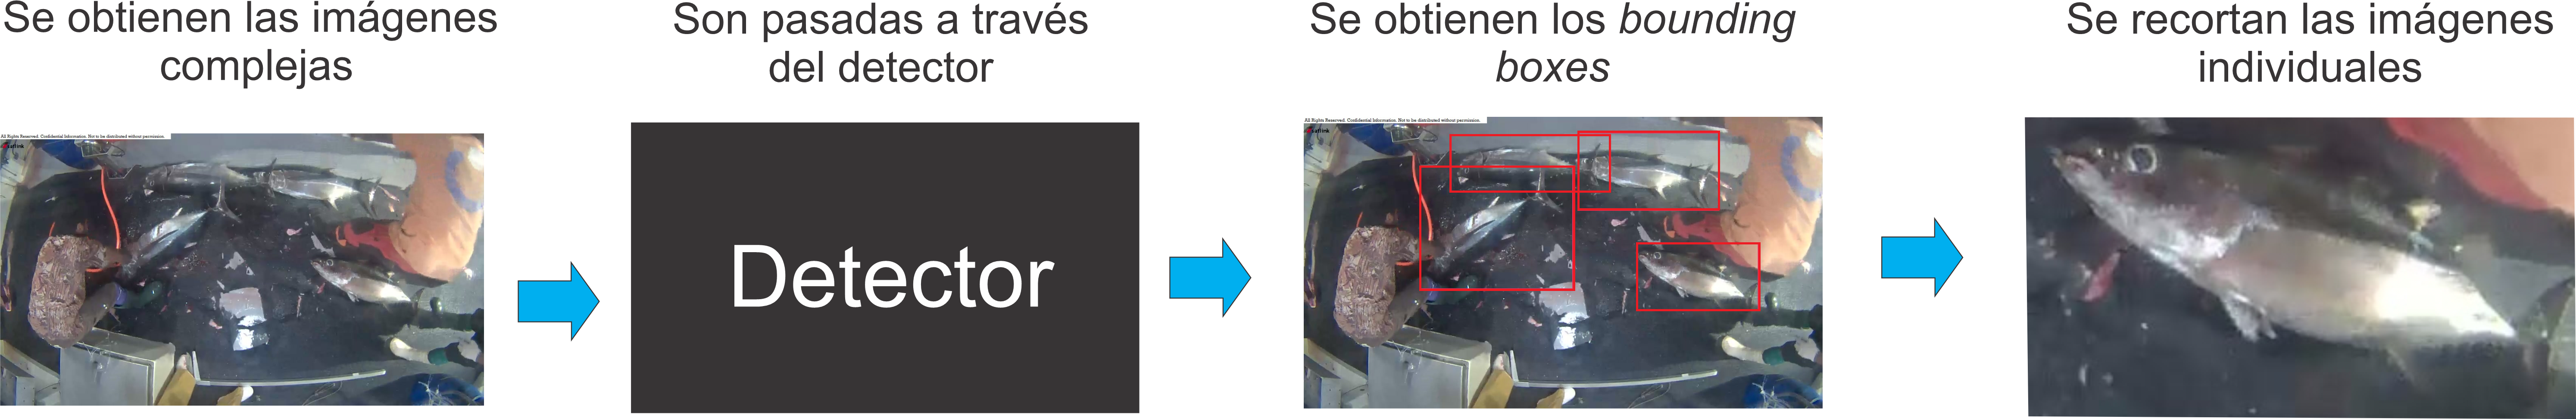
\includegraphics[width=1\textwidth]{images/detector_pez.png}
\caption{Flujo de entrada y salida del detector }
\label{fig:detector_pez}
\end{figure}



\section{Clasificador}
Una vez ubicados los peces, se recortaron y redimensionaron las imágenes para 
ajustarlas a la entrada que espera el clasificador. Para los experimentos, se 
utilizó la resolución específica para cada una de las redes a probar. Estas 
redes también fueron obtenidas con sus pesos pre-entrenados con 
``Imagenet". Se les aplicó TL, congelando todas las capas convolucionales. Por 
último, a cada uno de estos modelos se le añadió una capa llamada 
``\textit{GlobalAveragePooling}'' y unas nuevas capas clasificadoras. Esto tuvo 
la finalidad de disminuir el número de parámetros 
finales de la capa de clasificación, mejorar su precisión y reducir su tiempo 
de entrenamiento. El flujo se ve evidenciado en la imagen \ref{fig:clasificador_pez}.

\begin{figure}[h!]
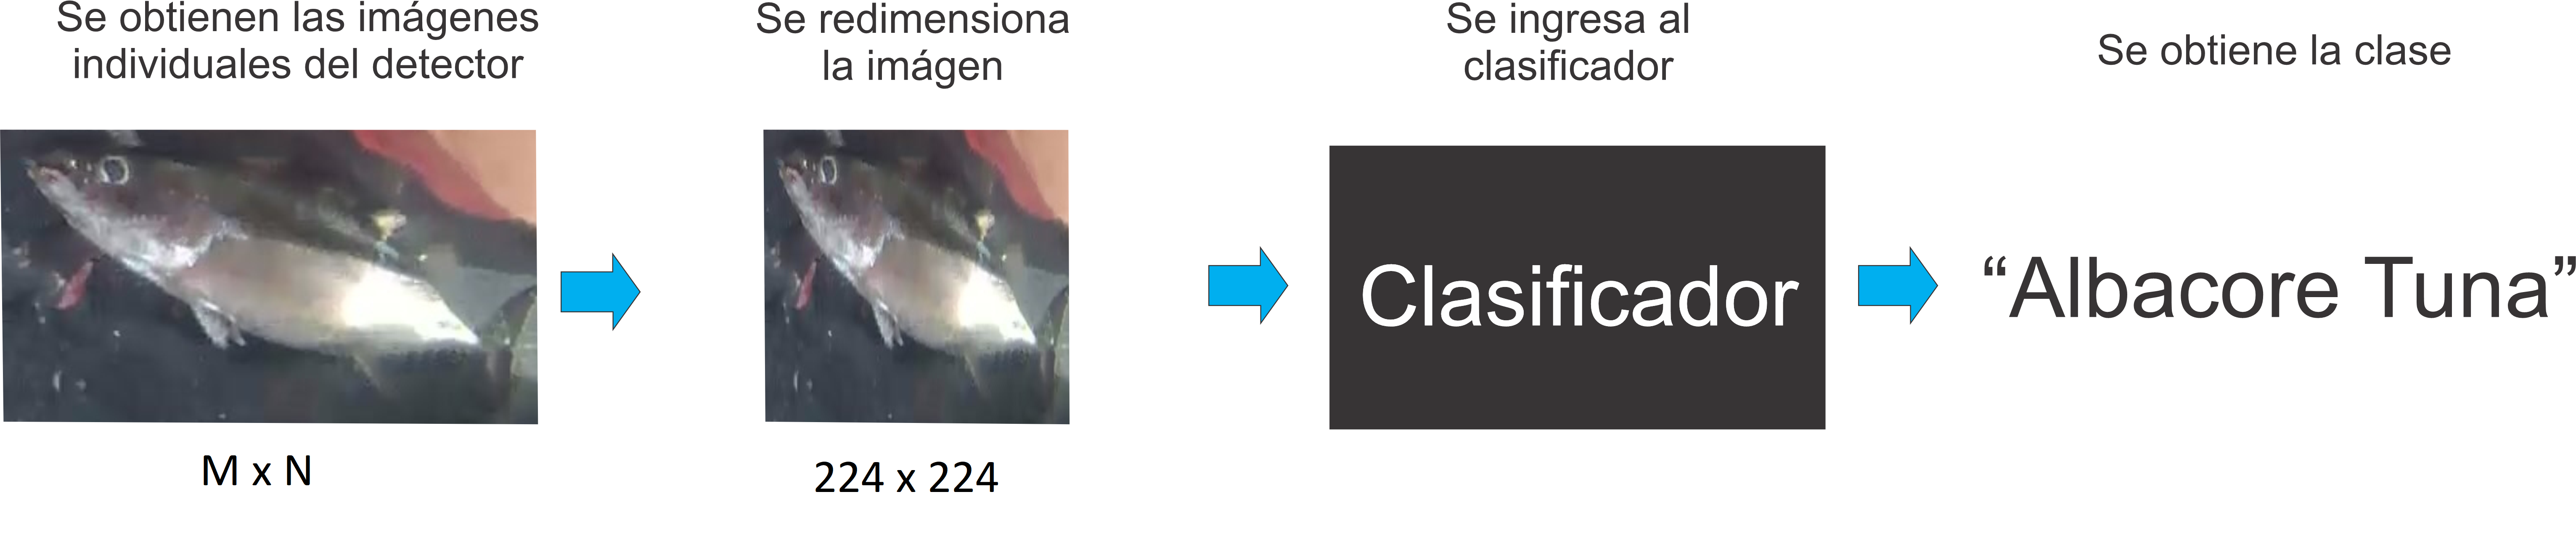
\includegraphics[width=1\textwidth]{images/clasificador_label.png}
\caption{Flujo de entrada y salida del clasificador }
\label{fig:clasificador_pez}
\end{figure}


\subsection{Evaluación de clasificadores para la experimentación}
En 2020, Orhan Yalsin \cite{DataModelos} realizó una resumen con algunas métricas para la 
evaluación de diferentes modelos de vanguardia, los cuales son mostrados 
en la tabla \ref{evaluación}. Nos basamos en sus resultados para seleccionar 
aquellos modelos que son mas eficientes tanto en tiempo, espacio y precisión.

\begin{table}[h!]
    \begin{tabular}{|l|r|r|r|r|r|}
    \hline
    \textbf{Model}                                               & \multicolumn{1}{l|}{\textbf{Size}} & \multicolumn{1}{l|}{\textbf{\begin{tabular}[c]{@{}l@{}}Top-1 \\ Accuracy\end{tabular}}} & \multicolumn{1}{l|}{\textbf{\begin{tabular}[c]{@{}l@{}}Top-5 \\ Accuracy\end{tabular}}} & \multicolumn{1}{l|}{\textbf{Parameters}} & \multicolumn{1}{l|}{\textbf{Depth}} \\ \hline
    Xception                                                     & 88 MB                              & 0.790                                                                                   & 0.945                                                                                   & 22,910,480                               & 126                                 \\ \hline
    VGG16                                                        & 528 MB                             & 0.713                                                                                   & 0.901                                                                                   & 138,357,544                              & 23                                  \\ \hline
    VGG19                                                        & 549 MB                             & 0.713                                                                                   & 0.900                                                                                   & 143,667,240                              & 26                                  \\ \hline
    ResNet50                                                     & 98 MB                              & 0.749                                                                                   & 0.921                                                                                   & 25,636,712                               & -                                   \\ \hline
    ResNet101                                                    & 171 MB                             & 0.764                                                                                   & 0.928                                                                                   & 44,707,176                               & -                                   \\ \hline
    ResNet152                                                    & 232 MB                             & 0.766                                                                                   & 0.931                                                                                   & 60,419,944                               & -                                   \\ \hline
    ResNet50V2                                                   & 98 MB                              & 0.760                                                                                   & 0.930                                                                                   & 25,613,800                               & -                                   \\ \hline
    ResNet101V2                                                  & 171 MB                             & 0.772                                                                                   & 0.938                                                                                   & 44,675,560                               & -                                   \\ \hline
    ResNet152V2                                                  & 232 MB                             & 0.780                                                                                   & 0.942                                                                                   & 60,380,648                               & -                                   \\ \hline
    InceptionV3                                                  & 92 MB                              & 0.779                                                                                   & 0.937                                                                                   & 23,851,784                               & 159                                 \\ \hline
    \begin{tabular}[c]{@{}l@{}}Inception\\ ResNetV2\end{tabular} & 215 MB                             & 0.803                                                                                   & 0.953                                                                                   & 55,873,736                               & 572                                 \\ \hline
    MobileNet                                                    & 16 MB                              & 0.704                                                                                   & 0.895                                                                                   & 4,253,864                                & 88                                  \\ \hline
    MobileNetV2                                                  & 14 MB                              & 0.713                                                                                   & 0.901                                                                                   & 3,538,984                                & 88                                  \\ \hline
    DenseNet121                                                  & 33 MB                              & 0.750                                                                                   & 0.923                                                                                   & 8,062,504                                & 121                                 \\ \hline
    DenseNet169                                                  & 57 MB                              & 0.762                                                                                   & 0.932                                                                                   & 14,307,880                               & 169                                 \\ \hline
    DenseNet201                                                  & 80 MB                              & 0.773                                                                                   & 0.936                                                                                   & 20,242,984                               & 201                                 \\ \hline
    NASNetMobile                                                 & 23 MB                              & 0.744                                                                                   & 0.919                                                                                   & 5,326,716                                & -                                   \\ \hline
    NASNetLarge                                                  & 343 MB                             & 0.825                                                                                   & 0.960                                                                                   & 88,949,818                               & -                                   \\ \hline
    EfficientNetB0                                               & 29 MB                              & 0.771                                                                                   & 0.933                                                                                   & 5,330,571                                & -                                   \\ \hline
    EfficientNetB1                                               & 31 MB                              & 0.791                                                                                   & 0.944                                                                                   & 7,856,239                                & -                                   \\ \hline
    EfficientNetB2                                               & 36 MB                              & 0.801                                                                                   & 0.949                                                                                   & 9,177,569                                & -                                   \\ \hline
    EfficientNetB3                                               & 48 MB                              & 0.816                                                                                   & 0.957                                                                                   & 12,320,535                               & -                                   \\ \hline
    EfficientNetB4                                               & 75 MB                              & 0.829                                                                                   & 0.964                                                                                   & 19,466,823                               & -                                   \\ \hline
    EfficientNetB5                                               & 118 MB                             & 0.836                                                                                   & 0.967                                                                                   & 30,562,527                               & -                                   \\ \hline
    EfficientNetB6                                               & 166 MB                             & 0.840                                                                                   & 0.968                                                                                   & 43,265,143                               & -                                   \\ \hline
    EfficientNetB7                                               & 256 MB                             & 0.843                                                                                   & 0.970                                                                                   & 66,658,687                               & -                                   \\ \hline
    \end{tabular}
    \caption{Evaluación de diferentes modelos. Tabla brindada por Orhan Yalcin \protect\cite{DataModelos}. }
    \label{evaluación}
\end{table}

\\
Esta tabla destaca varios modelos notables por su equilibrio entre 
tamaño, cantidad de parámetros y precisión. Entre ellos VGG19 
(si consideramos solo las capas convolucionales), ResNet50, InceptionV3, 
y los EfficientNetBX resultan tener una buena relación entre el peso, el 
número de parámetros y la precisión que estas obtienen, esta última 
siendo de las más altas dentro de todos estos modelos. Se tuvo en 
consideración la ejecución en videos en tiempo real y por ello se necesitó 
que el modelo sea el más pequeño posible evitando perder la precisión. Por 
otra parte, están las MobileNet, las cuales ya han sido utilizadas para el 
procesamiento de imágenes en tiempo real por ser más ligeras, enfocadas a 
ser utilizadas en celulares. Creemos que todas estas redes eran aptas para 
este problema y pasarán a ser evaluadas en el siguiente capítulo, en base 
al primer \textit{dataset} mencionado anteriormente. \\

Una vez analizado esas redes en base al \textit{dataset}, se compararon 
la precisión y costo entre ellas y se obtuvo la que finalmente pasará a 
formar parte del \textit{pipeline} final, en donde fue encargada de 
clasificar cada imagen obtenida por la red Yolo.\\

En el siguiente capítulo finalmente se verá la experimentación realizada con todos 
los modelos anteriormente señalados, tanto como la especificación de las 
imágenes y la experimentación del \textit{pipeline} final.

\section{\textit{Labeled Boxes}}
Una vez generadas las etiquetas del clasificador para cada una de las 
imágenes obtenidas por el detector, se procedió a asignar cada 
\textit{bounding box} con su etiqueta correspondiente. Terminado este 
trabajo, se obtuvo como salida la imagen con los \textit{labeled boxes} 
para cada instancia de pez que se encuentre. 

\begin{figure}[h!]
    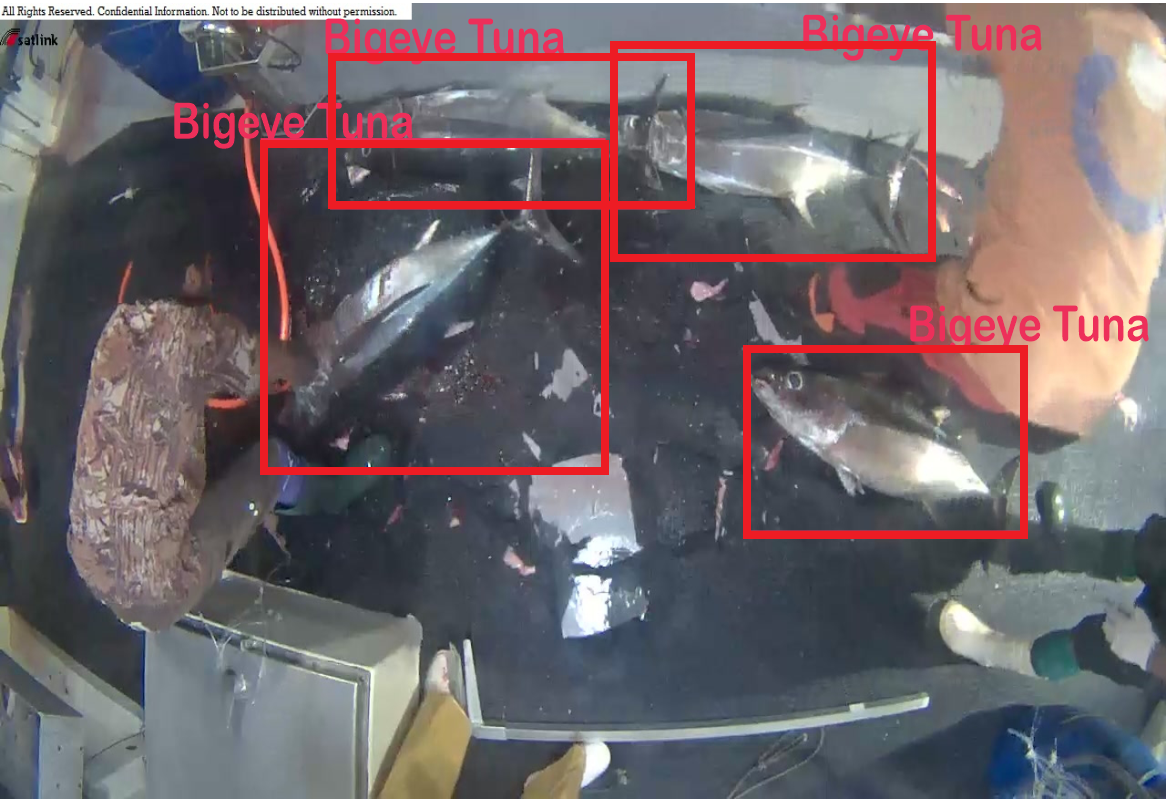
\includegraphics[width=1\textwidth]{images/BoundingBox.png}
    \caption{\textit{Labeled Boxes} dentro de la imagen ya procesada. }
    \label{fig:LabelBoxes}
\end{figure}

\chapter{RESULTADOS Y DISCUSI\'ON}

Habiendo expuesto cada uno de los pasos dentro de la metodología de la investigación en el capítulo anterior, 
en el presente capítulo se expondrán cada uno de los experimentos hechos de manera ordenada 
que se realizó. Primero se hablarán de los \textit{datasets} utilizados, los softwares y 
hardwares, el preprocesamiento de entradas. Finalmente, se abordarán los diferentes 
\textit{stages} del \textit{pipeline}, comenzando por el detector, luego el clasificador y 
terminando por el \textit{pipeline} completo.

\section{Aspectos generales}
\subsection{\textit{Datasets}}
Como ya había sido mencionado anteriormente, se utilizará un banco de imágenes de diferentes especies peruanas, las cuales fueron recogidas de  diferentes repositorios y competencias de la página \href{https://www.kaggle.com/}{\textit{Kaggle}}. Estos \textit{datasets}  contienen las imágenes de peces y sus \textit{labels}, los cuales representan las especies del pez que se encuentra dentro de la imagen. Se obtuvieron 3 diferentes \textit{datasets}, de entre los cuales se extrajeron únicamente las especies que también se encuentran en el mar peruano y de entre ellos, el primero se utilizará para la comprobación del \textit{pipeline} final, mientras que los otros dos se utilizaron para probar el clasificador. La lista de cada uno de los \textit{datasets} se encuentra a continuación:
\begin{itemize}
    \item \href{https://www.kaggle.com/c/the-nature-conservancy-fisheries-monitoring}{\textit{The Nature Conservancy Fisheries Monitoring}}: Concurso realizado en 2017 a través de la plataforma mencionado anteriormente. Contiene varias imágenes sobre las siguientes especies: atún blanco o ``bonito'', atún de ojo grande, atún de aleta amarilla y pez delfín o comúnmente llamado ``perico''.
    \item \href{https://www.kaggle.com/datasets/giannisgeorgiou/fish-species}{\textit{Fish Species}}: Contiene 2000 imágenes de cada una de las 20 especies del mediterráneo de entre las cuales se ha recolectado las imágenes de la lisa o ``Mugil cephalus'', el pez guitarra o ``Rhinobatos cemiculus'', la caballa o ``scomber japonicus'' y el pez espada o ``tetrapturus belone'' . 
    \item \href{https://www.kaggle.com/datasets/crowww/a-large-scale-fish-dataset}{\textit{A Large Scale Fish Dataset}}: Contiene 1000 imágenes de 9 especies diferentes encontradas en Turquía, de entre las cuales, una de ellas, la trucha marrón, también se encuentra en aguas peruanas. 
\end{itemize}

\subsection{Software y Hardware}
A lo largo de toda la experimentación, se utilizará un computador de escritorio con las siguientes características:

\begin{table}[h!]
\centering
\footnotesize
\begin{tabular}{|l|l|}
\hline
\textbf{Componente} & \textbf{Descripción} \\ \hline
Procesador & AMD Ryzen 7 3700X 8-Core 3.6 GHz. \\ \hline
Memoria RAM & Crucial Ballistix 16GB DDR4 - 3600MHZ \\ \hline
Tarjeta Gráfica & Nvidia RTX 2060 6GB \\ \hline
\end{tabular}
\end{table}

Por otra parte, se utilizó Python, junto con Keras, Sklearn y Tensorflow 
para el desarrollo del \textit{pipeline} en general y el pre y post 
procesamiento de los datos. Para el procesamiento de las imágenes (con Yolo) 
se utilizó OpenCV compilado con cudnn para la habilitación del uso de tarjeta gráfica. 

\subsection{Preprocesamiento de \textit{Bounding Boxes}}

Se llevó a cabo la creación manual de los \textit{bounding boxes} para todas las 
imágenes del \textit{dataset} ``\textit{The Nature Conservancy}'', utilizando el 
software de código abierto \textit{YoloLabel}, el cual proporciona una interfaz 
sencilla. Se contó con ayuda de un experto para crear los \textit{bounding boxes} 
y etiquetar cada imagen.
\\

Es importante mencionar que, aunque las imágenes en general eran borrosas, las del 
conjunto de entrenamiento resultaron ser menos complejas que las del conjunto de 
prueba. De hecho, estas últimas fueron difíciles de clasificar incluso para el 
experto. Una vez creados los \textit{bounding boxes}, se procedió a recortar las 
imágenes. Como resultado de este proceso, se obtuvieron diferentes cantidades de 
imágenes por clase, como se muestra en la tabla \ref{table:ImagenesNumero}:
\\
\begin{table}[h!]
\footnotesize
\centering
\begin{tabular}{|c|r|r|}
\hline
Especie                                                            & \multicolumn{1}{c|}{\begin{tabular}[c]{@{}c@{}}Número de\\ imágenes de\\ entrenamiento\end{tabular}} & \multicolumn{1}{c|}{\begin{tabular}[c]{@{}c@{}}Número de\\ imágenes de\\ prueba\end{tabular}} \\ \hline
\textit{\begin{tabular}[c]{@{}c@{}}Albacore \\ Tuna\end{tabular}}  & 2341                                                                                                 & 383                                                                                           \\ \hline
\textit{\begin{tabular}[c]{@{}c@{}}Bigeye \\ Tuna\end{tabular}}    & 288                                                                                                  & 391                                                                                           \\ \hline
\textit{Dolphinfish}                                               & 127                                                                                                  & 20                                                                                            \\ \hline
\textit{\begin{tabular}[c]{@{}c@{}}Moonfish \\ (LAG)\end{tabular}} & 98                                                                                                   & 59                                                                                            \\ \hline
\textit{Shark}                                                     & 300                                                                                                  & 131                                                                                           \\ \hline
\textit{\begin{tabular}[c]{@{}c@{}}Yellowfin \\ Tuna\end{tabular}} & 195                                                                                                  & 21                                                                                            \\ \hline
\textit{Other}                                                     & 778                                                                                                  & 164                                                                                           \\ \hline
\textit{\textbf{Total}}                                            & \textbf{4127}                                                                                        & \textbf{1169}                                                                                 \\ \hline
\end{tabular}
\caption{Número de imágenes por \textit{dataset}}
\label{table:ImagenesNumero}
\end{table}

Una observación crucial que debe ser mencionada es la presencia de heterogeneidad en 
ambos \textit{datasets}, lo cual se asemeja a la realidad, ya que algunos de los peces 
son más difíciles de capturar que otros. Por lo tanto, este caso de estudio también involucra otros desafíos, como clases desequilibradas y un número bajo de imágenes, lo que puede provocar \textit{overfitting} en muchos casos, ya que debido a la disparidad de clases y la complejidad de los modelos, existe la posibilidad que se categorice las clases con más instancias \cite{Overfitting}.

\section{Evaluación de Detectores }
En esta primera experimentación se realizarán pruebas con 3 diferentes modelos: Yolov5 
preentrenado con el \textit{dataset} ``Objects 365'', UniDet y Yolov5 entrenado con 
nuestro \textit{dataset}. Para ello, se obtuvo un conjunto aleatorio del 80\% y 20\% de 
las imágenes recortadas entre el conjunto de entrenamiento y prueba, mientras que para el 
entrenamiento del Yolov5, se utilizaron todos los datos de entrenamiento y prueba.

\subsection{Extracción de imágenes por el detector} 
Una vez obtenidos el 80\% y 20\% de las imágenes del \textit{dataset} 
``\textit{The Nature Conservancy}'' en donde se unificaron los \textit{datasets} de entrenamiento 
y prueba (acción que se justificará en la sección 5.4.1 y que está evidenciada en el anexo 
\ref{appendix}). se utilizaron tres diferentes detectores para el recorte de las imágenes. 
Para cada uno de ellos, se clasificaron los recortes por la etiqueta de la imagen de la cual 
fueron obtenidas y las que eran de prueba fueron nuevamente etiquetados por el experto. Por 
otra parte, todas las imágenes recortadas que no contenían un pez dentro, no estaban enfocadas 
o no contenían perfectamente al pez y fueron etiquetadas como errores. Para esta experimentación 
se utilizaron dos yolov5 (uno preentrenado con Objects365 y uno entrenado con el \textit{dataset}) 
y un UniDet, entrenado con COCO, Objects 365 y OpenImages. Los datos obtenidos fueron 
recopilados en la tabla \ref{table:peces}. Cabe resaltar que el yolov5 entrenado fue utilizado 
como detector general (ignorando las clases que predecía).
\\
\begin{table}[h!]
\footnotesize
\centering
\begin{tabular}{|c|r|r|r|}
\hline
\multicolumn{1}{|r|}{}                                                                                     & \multicolumn{1}{c|}{Peces detectados} & \multicolumn{1}{c|}{\begin{tabular}[c]{@{}c@{}}Otros objetos\\ (errores)\end{tabular}} & \multicolumn{1}{c|}{\textbf{Total}} \\ \hline
Real                                                                                                       & 1061                                  & -                                                                                     & \textbf{1061}                       \\ \hline
\begin{tabular}[c]{@{}c@{}}Predicted Yolov5\\ pretrained(40\%\\ threshold)\end{tabular}                    & 150                                   & 335                                                                                   & \textbf{485}                        \\ \hline
\begin{tabular}[c]{@{}c@{}}Predicted UniDet\\ pretrained (no \\ threshold)\end{tabular}                    & 426                                   & 124                                                                                   & \textbf{550}                        \\ \hline
\begin{tabular}[c]{@{}c@{}}Predicted Yolov5\\ trained (freezed \\ backbone 95\% \\ threshold)\end{tabular} & 843                                   & 399                                                                                   & \textbf{1233}                       \\ \hline
\end{tabular}
\caption{Número de peces vs errores detectados por cada modelo}
\label{table:peces}
\end{table}

Como se esperaba, utilizar un modelo preentrenado no especializado en detectar una clase específica, genera una menor precisión en comparación de uno que sí está entrenado, y más aún, si ese \textit{dataset} es el que está usando para clasificar. Se utilizaron dos métricas para el análisis de estos datos: el porcentaje de peces detectados con respecto del \textit{dataset} original y el porcentaje de error general obtenido por cada detección. Estos resultados se pueden ver en la tabla \ref{table:pecesPorcentaje}.
\\

\begin{table}[h!]
\footnotesize
\centering
\begin{tabular}{|c|r|r|}
\hline
\multicolumn{1}{|r|}{}                                                                                     & \multicolumn{1}{c|}{\begin{tabular}[c]{@{}c@{}}Porcentaje de\\ peces detectados\end{tabular}} & \multicolumn{1}{c|}{\begin{tabular}[c]{@{}c@{}}Porcentaje de errores\\ detectados del total\end{tabular}} \\ \hline
\begin{tabular}[c]{@{}c@{}}Predicted Yolov5\\ pretrained(40\%\\ threshold)\end{tabular}                    & 14.13\%                                                                                       & 69.07\%                                                                                                   \\ \hline
\begin{tabular}[c]{@{}c@{}}Predicted UniDet\\ pretrained (no \\ threshold)\end{tabular}                    & 40.15\%                                                                                       & \textbf{22.54\%}                                                                                                   \\ \hline
\begin{tabular}[c]{@{}c@{}}Predicted Yolov5\\ trained (freezed \\ backbone 95\% \\ threshold)\end{tabular} & \textbf{79.45\%}                                                                                       & 32.36\%                                                                                                   \\ \hline
\end{tabular}
\caption{Porcentaje de detecciones correctas vs errores generados }
\label{table:pecesPorcentaje}
\end{table}

Se puede ver una baja precisión por parte del Yolov5 preentrenado, lo cual es comprensible considerando que no ha sido preentrenado especialmente para detectar peces, sino con un \textit{dataset} genérico y es un modelo bastante ligero. UniDet, en cambio, es un modelo mucho más complejo, y tiene 3 detectores internamente (uno para cada dataset), los cuales en conjunto predicen la clase final del objeto y es por lo cual generan un mejor resultado que el anterior pero a un costo mucho mayor. Finalmente el Yolov5 entrenado específicamente con el \textit{dataset} obtenido muestra una especialización en la detección de estos individuos que finalmente logra un 79.45\% de precisión. Aún así se necesita considerar el hecho que el entrenamiento de este modelo tomo alrededor de 80 minutos, siendo este aproximadamente 13 veces más el tiempo que le toma entrenar a un modelo como lo es EfficientnetB0 con un bajo número de imágenes(4300 imágenes, a comparación de 5300 para el CNN).
\\

Además, al considerar el porcentaje de errores generados, se observa que UniDet produce 
una menor cantidad de detecciones incorrectas en comparación con YOLOv5 preentrenado y 
YOLOv5 entrenado, lo que demuestra que es un modelo más robusto. Sin embargo, debido a 
la falta de especialización durante su entrenamiento, UniDet ofrece resultados más pobres 
en las detecciones. En este sentido, se cree que si tuviéramos los pesos de un modelo 
específicamente entrenado para la detección de peces, se mejoraría el resultado y se 
evitaría la necesidad de entrenar uno desde cero o utilizar uno que haya sido entrenado 
de manera genérica. Esto aumentaría la precisión general del sistema y tendría un 
impacto positivo en el flujo de trabajo.
\\

\section{Evaluación de Desempeño de Diferentes Clasificadores}
En la presente sección se realizarán dos experimentos para poder seleccionar una arquitectura que será utilizada para actuar como nuestro clasificador dentro del \textit{pipeline} final. Para ello, se compararán algunas arquitecturas del estado del arte utilizando los 3 \textit{datasets}, analizando tanto las pérdidas y precisión en \textit{training}, \textit{validation} y \textit{testing} para cada uno, así como la velocidad por batch (8 imágenes) y el número de épocas necesarias para entrenar dichas arquitecturas. 
\subsection{Arquitectura general}
Como fue mencionado, para la creación de cada una de las arquitecturas se utilizarán modelos ya preentrenados del estado del arte, a los cuales se les aplicará TL para su entrenamiento con nuestro \textit{dataset}. Este proceso consistirá en congelar todas las capas convolucionales, para luego ser pasado por una capa de \textit{GlobalAveragePooling2D}, luego por una \textit{Flatten}, la cual pasa de un formato bidimensional a uno unidimensional y luego por las siguientes tres capas: 
\begin{itemize}
    \item \textit{BatchNormalization}
    \item \textit{Dropout} de 50\%
    \item Capa densa a X \textit{outputs} con una función de activación RELU o softmax, dependiendo si es una capa oculta o la de salida.  
    \item 8 imágenes por batch 
\end{itemize}

Estas tres capas son ejecutadas para cada uno de los siguientes tamaños: 
$$[1024,256,64,LABELS\_SIZE], donde $$
LABELS\_SIZE representará el número de clases de salida que generará el clasificador.  

\subsection{Experimentación \#1}

Para el primer análisis, se utilizaron las consideraciones anteriores para comparar las diferentes arquitecturas del estado del arte mencionadas en el anterior capítulo. Para esta comparación, se utilizaron las imágenes obtenidas de los \textit{datasets} \textit{Fish Species} y \textit{A Large Scale Fish Dataset} combinados y se compararon los resultados de las métricas obtenidas. 
La primera de las métricas a comparar serán las gráficas de pérdida. En la figura \ref{fig:losses1} se ilustra una comparativa de la disminución de la pérdida con respecto al tiempo (épocas).

\begin{figure}[h!]
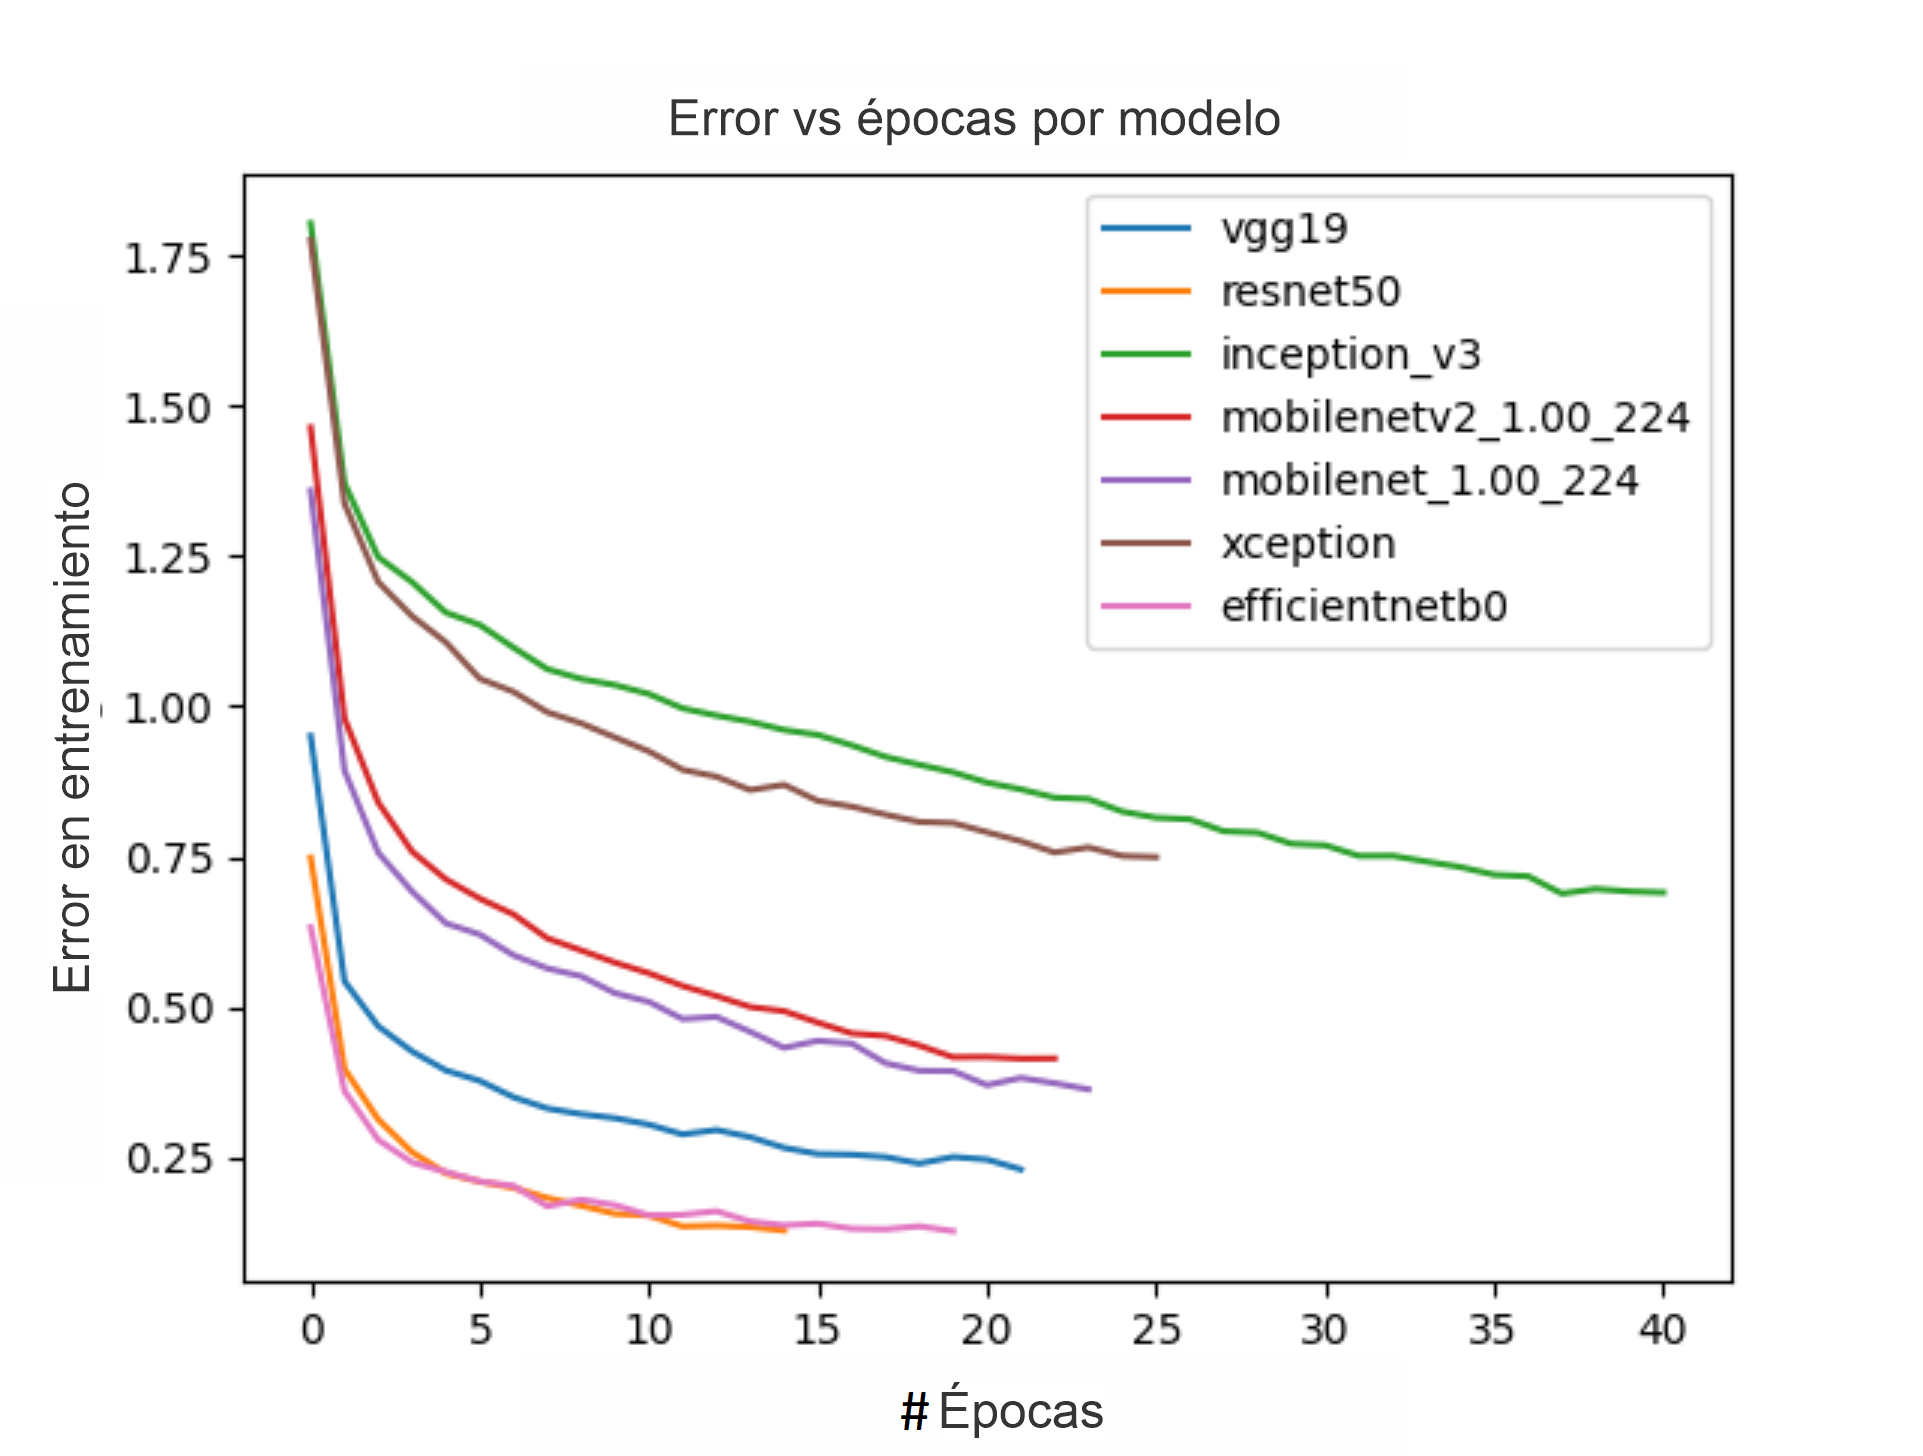
\includegraphics[width=1\textwidth]{images/loss1.png}
\centering
\caption{Gráfica comparativa de la pérdida entre todos los modelos a estudiar}
\label{fig:losses1}
\end{figure}


En esta gráfica se puede ver que los modelos que consiguen mejores descensos en esta 
métrica son tanto Resnet50, Vgg19 y EfficientnetB0, lo cual era bastante esperado conforme 
a la teoría, salvo por el Vgg19. Otro detalle interesante que salió a relucir de esta 
experimentación fue que InceptionV3 y Xception tuvieron una pérdida bastante elevada, 
contrario a lo que se esperaba en un inicio, lo cual podría ser motivo de análisis en un 
futuro para saber cuales fueron los motivos por los cuales no consiguieron aprender del 
\textit{dataset}. Por último, se puede ver como las dos MobileNet están en el medio de 
todas las demás redes analizadas, lo cual, es un dato a resaltar considerando lo ligero que 
son. \\

También se obtuvieron las siguientes métricas que fueron recopiladas en la tabla \ref{table:data1}.

\begin{table}[h!]
\footnotesize
\centering
\begin{tabular}{|c|c|c|c|c|c|c|}
\hline
\textbf{} & \textbf{\begin{tabular}[c]{@{}c@{}}Precisión\\en\\training\end{tabular}} & \textbf{\begin{tabular}[c]{@{}c@{}}Precisión \\ en \\ validation\end{tabular}} & \textbf{\begin{tabular}[c]{@{}c@{}}Precisión \\ en \\testing\end{tabular}} & \textbf{\begin{tabular}[c]{@{}c@{}}Perdida \\ final en \\ training\end{tabular}} & \textbf{\begin{tabular}[c]{@{}c@{}}Velocidad \\ por batch\\ (8 \\imágenes) \\ en ms\end{tabular}} & \textbf{\begin{tabular}[c]{@{}c@{}}Número \\ de\\ épocas\end{tabular}} \\ \hline
\textbf{Vgg19} & 0.9193 & 0.9928 & 0.9926 & 0.2299 & 71 & 21 \\ \hline
\textbf{Resnet50} & \textbf{0.9596} & \textbf{0.9993} & 0.9950 & 0.1282 & 52 & 14 \\ \hline
\textbf{\begin{tabular}[c]{@{}c@{}}Inception\\V3\end{tabular}} & 0.7362 & 0.6620 & 0.6681 & 0.6901 & 42 & 40 \\ \hline
\textbf{\begin{tabular}[c]{@{}c@{}}MobileNet\\V2\end{tabular}} & 0.8521 & 0.9052 & 0.9104 & 0.4143 & 28 & 31 \\ \hline
\textbf{\begin{tabular}[c]{@{}c@{}}MobileNet\\V1\end{tabular}} & 0.8694 & 0.9288 & 0.9519 & 0.3628 & \textbf{23} & 23 \\ \hline
\textbf{Xception} & 0.7244 & 0.7085 & 0.7178 & 0.7490 & 48 & 25 \\ \hline
\textbf{\begin{tabular}[c]{@{}c@{}}EfficientNet\\B0\end{tabular}} & 0.9577 & \textbf{0.9993} & \textbf{1.0000} & \textbf{0.1270} & 41 & \textbf{19} \\ \hline
\end{tabular}
\caption{Datos recopilados de la prueba de diferentes modelos del estado del arte}
\label{table:data1}
\end{table}


Esta tabla también proporciona datos interesantes sobre la experimentación. En primer lugar, 
Vgg19 tuvo la mayor pérdida entre todos los modelos, pero logró una precisión bastante 
aceptable en términos de entrenamiento, mientras que su precisión en validación y prueba 
fue casi perfecta. En segundo lugar, siguiendo con el análisis anterior, se observa que 
InceptionV3 y Xception obtuvieron resultados acordes a su pérdida en términos de precisión 
general. \\

Otro punto a resaltar es el hecho que ambos MobileNet obtienen un resultado bastante similar 
en términos de precisión en general, pero MobileNetV2 obtiene una pequeña diferencia, la cual 
la hace mejor que su versión anterior, pero a un costo en términos de velocidad, lo cual 
también se esperaba conforme a la teoría. Por último, cabe señalar que los tres modelos que 
obtuvieron la mejor precisión en pruebas fueron EfficientnetB0, Resnet50 y Vgg19 respectivamente.\\
A manera de conclusión, se pudo ver que con un \textit{dataset} relativamente sencillo, se puede obtener resultados bastante favorables, que logran casi a su totalidad automatizar este tipo de problemas con modelos ya pre-entrenados que son facilmente modificables para su uso.

\subsection{Experimentación \#2}

Para este segundo análisis, se  utilizaron las imágenes obtenidas del \textit{datasets} 
\textit{The Nature Conservancy Fisheries Monitoring}. Dentro de estas imágenes se podrían 
encontrar muchos peces de la misma especie por imagen. En ese sentido la labor del 
clasificador será identificar si esta imagen contiene ejemplares de un determinado 
pez en ella. Para este experimento, únicamente se tomaron los \textit{datasets} de 
entrenamiento y validación, ya que el de testeo no contenía etiquetas, pero será 
utilizado en futuras experimentaciones.  De la misma manera que en la anterior 
experimentación, primero se procederá a analizar las gráficas de error, tal como se 
ven en la imagen \ref{fig:losses2}.

\begin{figure}[h!]
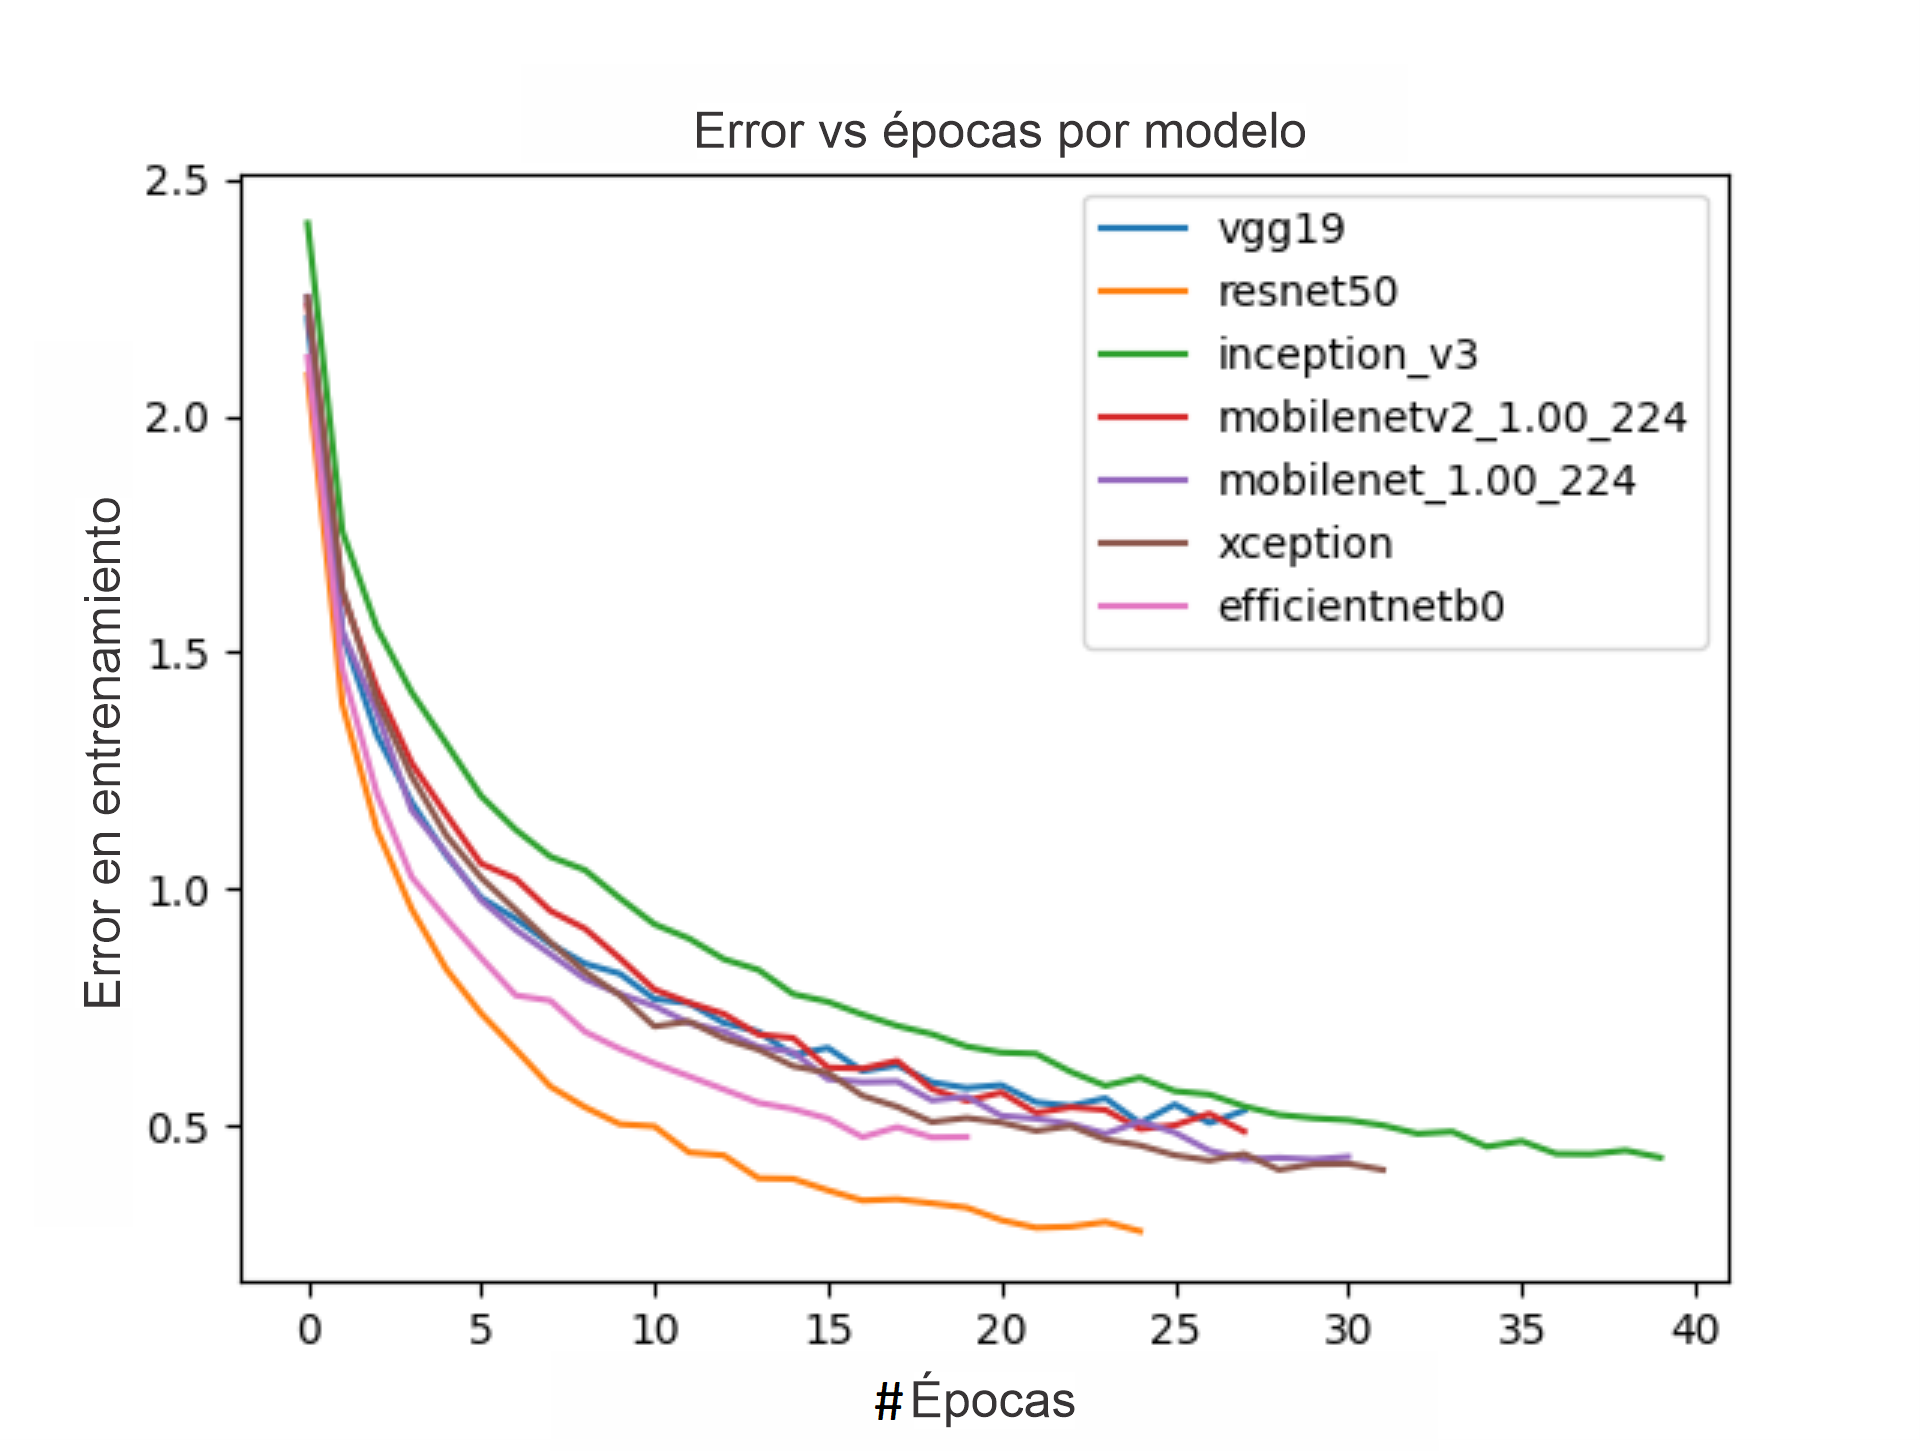
\includegraphics[width=1\textwidth]{images/loss2.png}
\centering
\caption{Gráfica comparativa de la perdida entre todos los modelos a estudiar}
\label{fig:losses2}
\end{figure}

Se puede ver que en esta experimentación se tuvieron rangos de error más elevados que el anterior, esto debido a la complejidad de la tarea. También se puede ver un descenso del error bastante más parejo entre todos los modelos experimentados. Nuevamente aparecen Resnet50 y Efficientnet con los menores resultados y también un menor número de épocas necesitadas para este entrenamiento.\\
Ahora pasaremos a analizar las métricas obtenidas para estos modelos, los cuales están plasmados en la tabla \ref{table:data2}.
\newpage
\begin{table}[h!]
\footnotesize
\centering
\begin{tabular}{|c|c|c|c|c|c|}
\hline
\textbf{} & \textbf{\begin{tabular}[c]{@{}c@{}}Precisión\\  en training\end{tabular}} & \textbf{\begin{tabular}[c]{@{}c@{}}Precisión \\ en \\ validation\end{tabular}} & \textbf{\begin{tabular}[c]{@{}c@{}}Perdida \\ final en \\ training\end{tabular}} & \textbf{\begin{tabular}[c]{@{}c@{}}Velocidad \\ por batch\\ ( 8 \\imágenes) \\ en ms\end{tabular}} & \textbf{\begin{tabular}[c]{@{}c@{}}Número \\ de\\ épocas\end{tabular}} \\ \hline
\textbf{Vgg19} & 0.8173 & 0.9061 & 0.5317 & 68 & 29 \\ \hline
\textbf{Resnet50} & \textbf{0.9139} & \textbf{0.9219} & \textbf{0.2769} & 50 & 24 \\ \hline
\textbf{\begin{tabular}[c]{@{}c@{}}Inception \\ V3\end{tabular}} & 0.8510 & 0.8637 & 0.4324 & 42 & 39 \\ \hline
\textbf{\begin{tabular}[c]{@{}c@{}}MobileNet\\V2\end{tabular}} & 0.8348 & 0.8516 & 0.4875 & 28 & 27 \\ \hline
\textbf{\begin{tabular}[c]{@{}c@{}}MobileNet\\V1\end{tabular}} & 0.8543 & 0.8743 & 0.4340 & \textbf{24} & 30 \\ \hline
\textbf{Xception} & 0.8676 & 0.8267 & 0.4065 & 48 & 31 \\ \hline
\textbf{\begin{tabular}[c]{@{}c@{}}EfficientNet\\B0\end{tabular}} & 0.8467 & \textbf{0.9101} & 0.4759 & 41 & \textbf{19} \\ \hline
\end{tabular}
\caption{Datos recopilados de la prueba de diferentes modelos del estado del arte}
\label{table:data2}
\end{table}

En comparación con la gráfica anterior, se observa un deterioro en todas las métricas 
\obtenidas. Resnet y Efficientnet mostraron una alta precisión en entrenamiento y validación, 
superando a Vgg19, el cual no obtuvo una buena precisión en entrenamiento y presentó una alta 
pérdida final, lo cual sugiere que sufrió de \textit{overfitting}. Si consideramos además 
la relación entre precisión y eficiencia, ambas MobileNet resultan bastante robustas, ya 
que generan una precisión relativamente alta, manteniendo una velocidad por \textit{batch} 
razonable. Exceptuando ambas MobileNets, InceptionV3 y EfficiententB0 fueron las que obtuvieron 
una velocidad por \textit{batch} menor que las demás. Por último cabe resaltar que Resnet50 
y Efficientnet fueron las redes que necesitaron un menor número de épocas para detenerse. 
\\

Considerando los resultados obtenidos, proponemos el uso de EfficientnetB0 para la creación del \textit{pipeline}, debido a su alta precisión tanto en las pruebas como en el entrenamiento, así como en la validación y prueba. Además, es significativamente más ligero, presenta una curva de aprendizaje más estable a lo largo de las épocas, un menor número de épocas necesitadas para entrenarse y una velocidad superior a todas las demás.

\section{Experimentación del clasificador}

En esta sección se llevaron a cabo 5 experimentos con el objetivo de validar y 
obtener un modelo entrenado basado en la arquitectura seleccionada en la sección anterior, 
con el fin de maximizar la precisión al entrenarlo con las imágenes recortadas. Dos de los 
experimentos se realizaron debido a una distribución inadecuada de los datos entre el 
\textit{dataset} de entrenamiento y el de pruebas. Estos dos experimentos se separaron y se 
mencionan en la sección de anexos para evitar interferencias con la continuidad de los demás 
experimentos.
\subsection{Experimentación \#1 (training/validation)}

En el primer experimento se emplearon únicamente las imágenes recortadas del \textit{dataset} 
de entrenamiento para comprobar la capacidad de aprendizaje del modelo. De estas imágenes, 
se seleccionó una parte para ser utilizada como conjunto de validación. En esta prueba, 
se llevaron a cabo 10 iteraciones utilizando el algoritmo de K-Fold para la muestra y se 
obtuvieron los resultados que se presentan en la tabla \ref{table:KFolds1}
\\

\begin{table}[h!]
\footnotesize
\centering
\begin{tabular}{|r|r|r|r|r|}
\hline
\textit{K} & \textit{training loss} & \textit{training accuracy} & \textit{validation loss} & \textit{validation accuracy} \\ \hline
1    & 0.0115      & 99.660\%    & 0.2697    & 94.43\%  \\ \hline
2    & 0.0011      & 100.00\%   & 0.2243    & 96.06\%  \\ \hline
3    & 0.0106      & 99.690\%    & 0.2106    & 95.13\%  \\ \hline
4    & 0.0186      & 99.510\%    & 0.2286    & 93.97\%  \\ \hline
5    & 0.0069      & 99.820\%    & 0.2265    & 95.36\%  \\ \hline
6    & 0.0060      & 99.820\%    & 0.1204    & 97.22\%  \\ \hline
7    & 0.0079      & 99.870\%    & 0.2417    & 91.88\%  \\ \hline
8    & 0.0147      & 99.640\%    & 0.2182    & 93.50\%  \\ \hline
9    & 0.0154      & 99.430\%    & 0.2767    & 93.27\%  \\ \hline
10   & 0.0327      & 98.920\%    & 0.2814    & 93.26\%  \\ \hline
\textbf{\textit{mean $\pm$ std}}     & \textbf{0.0125$\pm$0.0087}      & \textbf{99.636$\pm$0.304\%}    & \textbf{0.2298$\pm$0.0461}    & \textbf{94.41$\pm$1.567\%}  \\ \hline
\end{tabular}
\caption{Perdida y precisión de entrenamiento y validación}
\label{table:KFolds1}
\end{table}
Con estos resultados, podemos observar que al ejecutar el mismo modelo varias veces, se 
obtienen resultados similares, lo que demuestra que no hay \textit{overfitting} y que el 
modelo no ha sido influenciado por la aleatoriedad en la inicialización de los pesos. Además, 
al evaluar imágenes de manera individual, se logra aumentar la precisión del modelo en 
comparación con la clasificación de imágenes completas.
\\

A continuación, se procedió a experimentar con el \textit{dataset} de \textit{testing} para 
poder comprobar si el modelo generó buenos resultados al predecir las clases de las imágenes 
recortadas. Por el contrario, se comprobó que pertenecían a distribuciones de datos muy 
diferentes. En el \textit{dataset} de prueba se tenían imágenes en diferentes entornos, con 
menor visibilidad y mayor falta de características distintivas de las especies estudiadas, 
entre otros factores que dificultaban el aprendizaje. Para poder comprobarlo, se realizaron 
las experimentaciones A y B (detalladas en el anexo \ref{appendix}). Se obtuvo que el modelo 
predijo a las imágenes complejas como ``bonito'' (\textit{Albacore Tuna}), ya que en el 
\textit{dataset} de entrenamiento había una mayor cantidad de estas imágenes, por lo que era 
estadísticamente más probable acertar de ese modo. Además, estas imágenes eran las que 
presentaban más defectos dentro del conjunto. En ese sentido se cambio el enfoque de las 
experimentaciones siguientes.

\subsection{Expermientación \#2 (extracción de datasets desde \textit{training}) }
Considerando lo anteriormente expuesto, se decidió dividir el conjunto de datos de entrenamiento en tres conjuntos diferentes: entrenamiento, validación y prueba, utilizando una proporción del 70\% para entrenamiento, 20\% para validación y 10\% para pruebas. El objetivo de esta nueva división fue comprobar si la suposición previa de que el problema era causado por el uso de conjuntos de datos con diferentes distribuciones era correcta. Los resultados obtenidos se muestran en la tabla \ref{table:Results4}.
\\
\begin{table}[h!]
\footnotesize
\centering
\begin{tabular}{|r|r|r|r|r|r|}
\hline
           & \multicolumn{1}{c|}{\textit{Loss}} & \multicolumn{1}{c|}{\textit{Balanced accuracy}} & \multicolumn{1}{c|}{\textit{F1-weighted}} & \multicolumn{1}{c|}{\textit{Precision}} & \multicolumn{1}{c|}{\textit{Recall}} \\ \hline
\textit{Train}      & 0.10                      & 96.57\%                        & 96.57\%                 & 96.76\%                         & 96.39\%                     \\ \hline
\textit{Validation} & 0.22                      & 95.64\%                        & 95.70\%                 & 95.75\%                         & 95.65\%                     \\ \hline
\textit{Testing}    & 0.23                      & 90.28\%                       & 95.29\%                & 95.39\%                       & 95.14\%                    \\ \hline
\end{tabular}
\caption{Estadísticos obtenidos del experimento \#2}
\label{table:Results4}
\end{table}

Se puede observar un comportamiento similar al experimento \#1, lo cual nos afirma entonces que realmente era un problema de malas distribuciones de datos en ambos \textit{datasets}. De la misma manera, se revisaron las matrices de confusión de los datos, los cuales se recopilaron en la tabla \ref{fig:Matrix2}

\begin{figure}[h!]
\centering
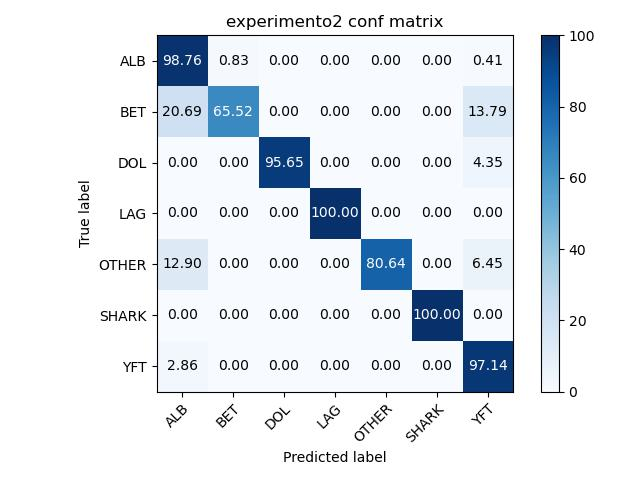
\includegraphics[width=0.8\textwidth]{images/experimento2_conf_matrix.jpg}
\caption{Matriz de confusión generada por el experimento \#2 en porcentajes}
\label{fig:Matrix2}
\end{figure}

Como se puede apreciar en la matriz de confusión, en general se obtuvo una buena precisión en la mayoría de las clases, excepto en la clase ``Bigeye Tuna'', lo cual es comprensible ya que se trata de una especie bastante similar al ``\textit{Albacore Tuna}'' y las imágenes no permiten apreciar las características diferenciales con claridad, como se pueden apreciar en las imágenes \ref{fig:combined2}.

\begin{figure}[h!]%
    \centering
    \subfloat[\centering Imagen de un ``bonito'' o ``\textit{Albacore Tuna}'' ]{{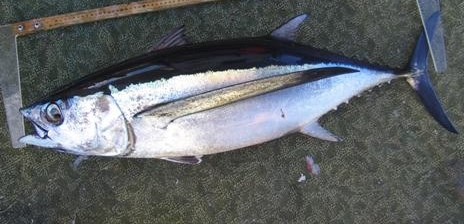
\includegraphics[width=5cm]{images/albacore.jpg} }}%
    \qquad
    \subfloat[\centering Imagen de un ``\textit{Bigeye Tuna}'']{{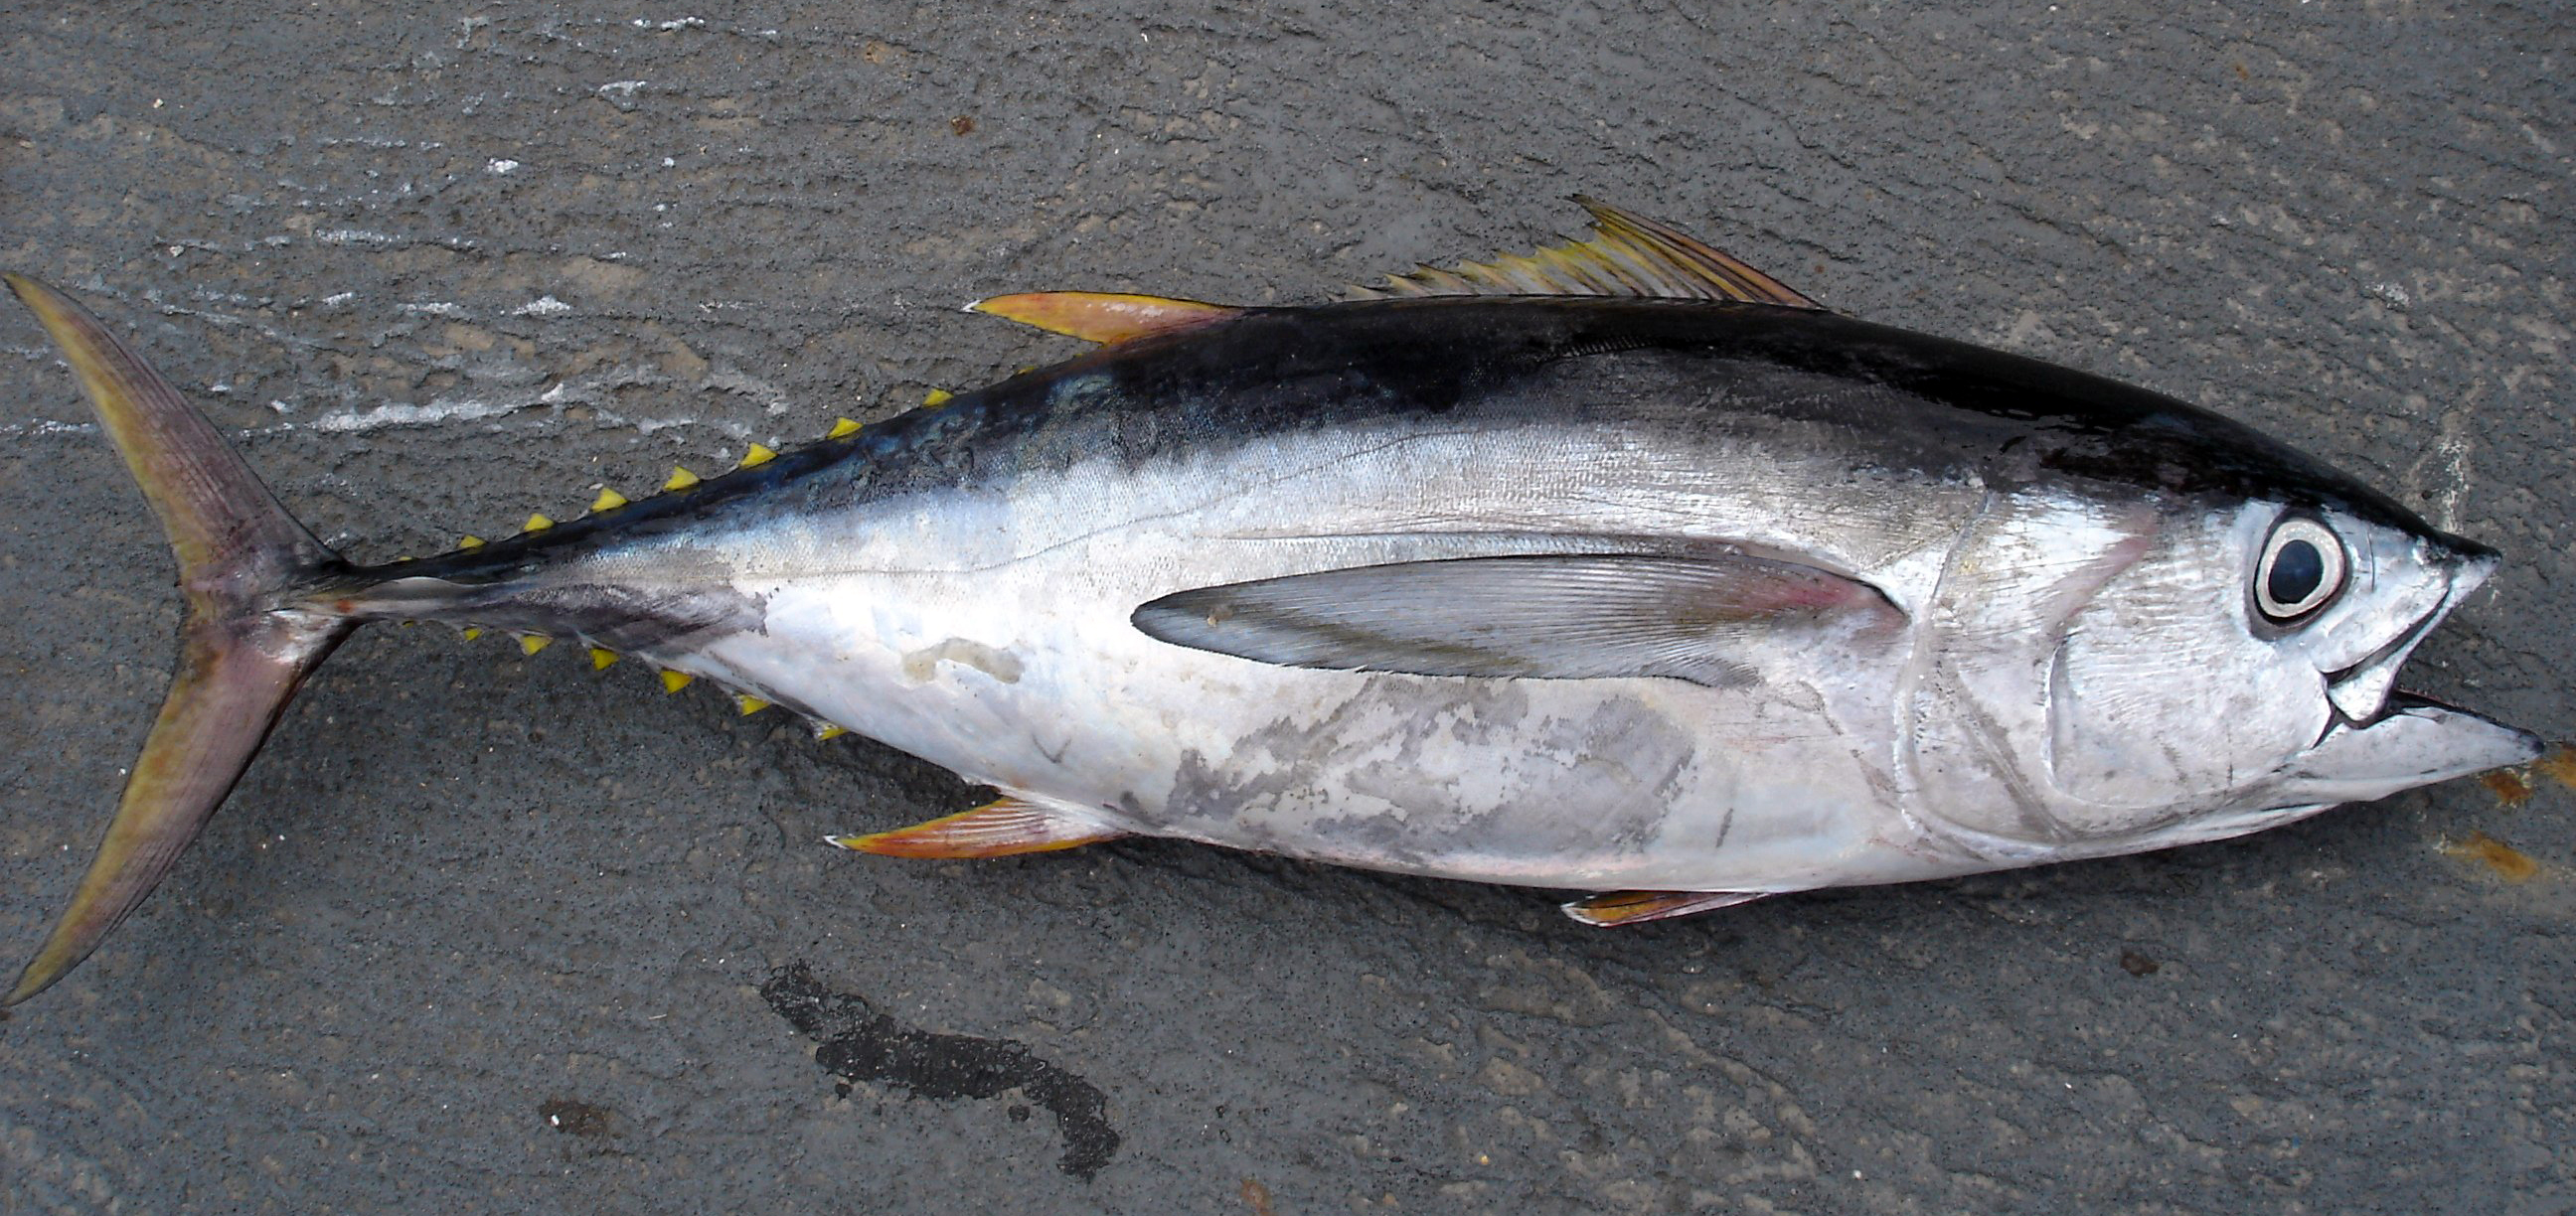
\includegraphics[width=5cm]{images/bigeye.jpg} }}%
    \caption{Comparación entren el ``\textit{Albacore Tuna}'' o bonito y el ``Bigeye Tuna''}%
    \label{fig:combined2}%
\end{figure}

 Además, se puede observar que no existe \textit{overfitting}, ya que las clases con menor cantidad de imágenes también consiguieron una alta precisión. También se revisaron las gráficas de pérdida y precisión tanto para el conjunto de entrenamiento como para el de validación, las cuales se muestran en las figuras \ref{fig:losses4} y \ref{fig:accuracy4}.
\\
\begin{figure}[h!]
\centering
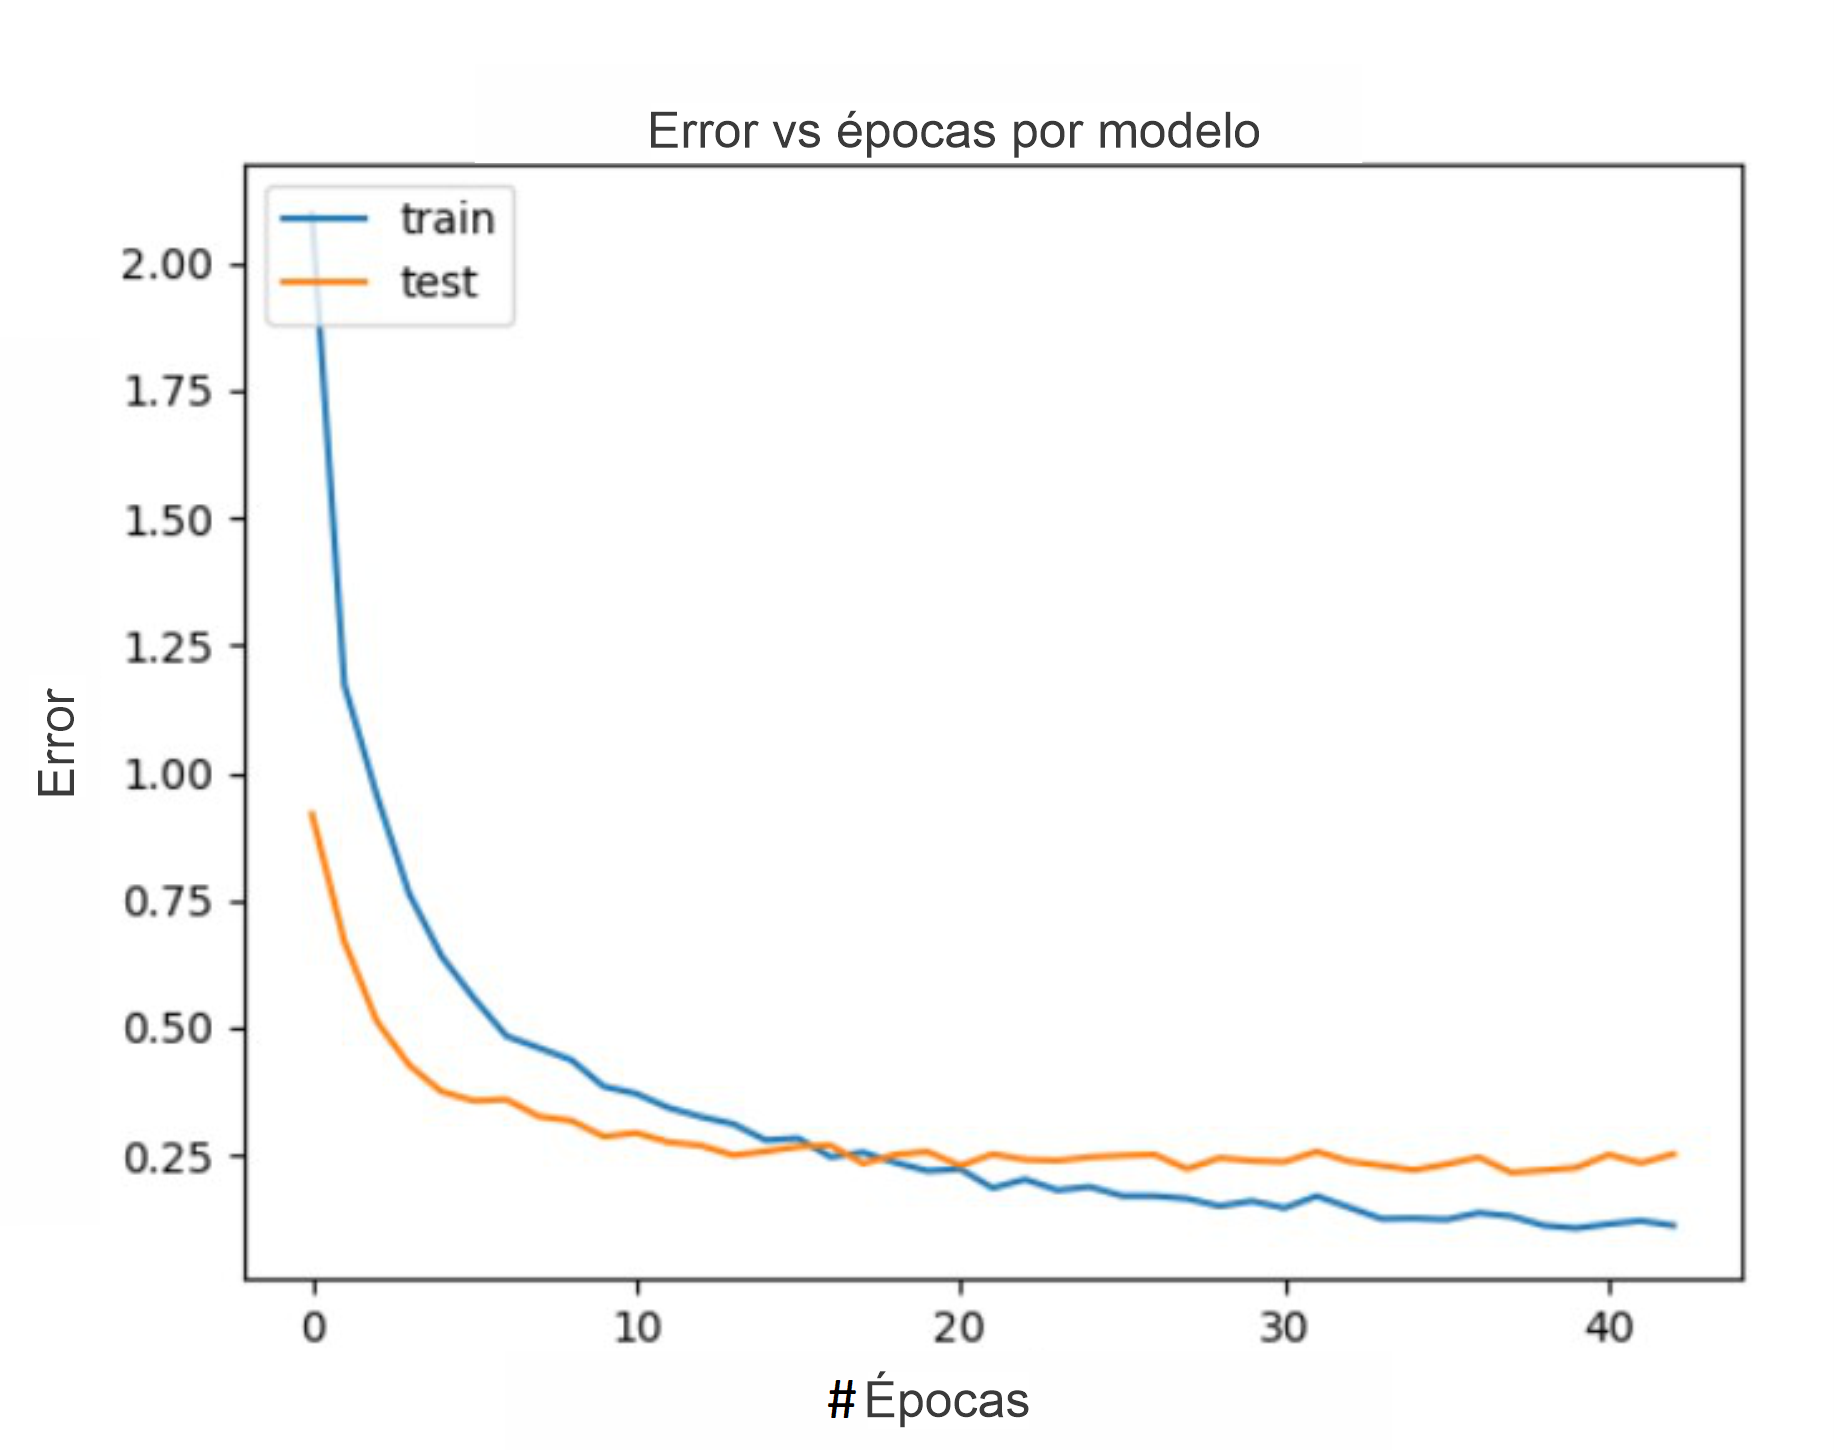
\includegraphics[width=0.8\textwidth]{images/loss4.png}
\caption{Gráfica comparativa de la perdida de entrenamiento y validacion}
\label{fig:losses4}
\end{figure}

\begin{figure}[h!]
\centering
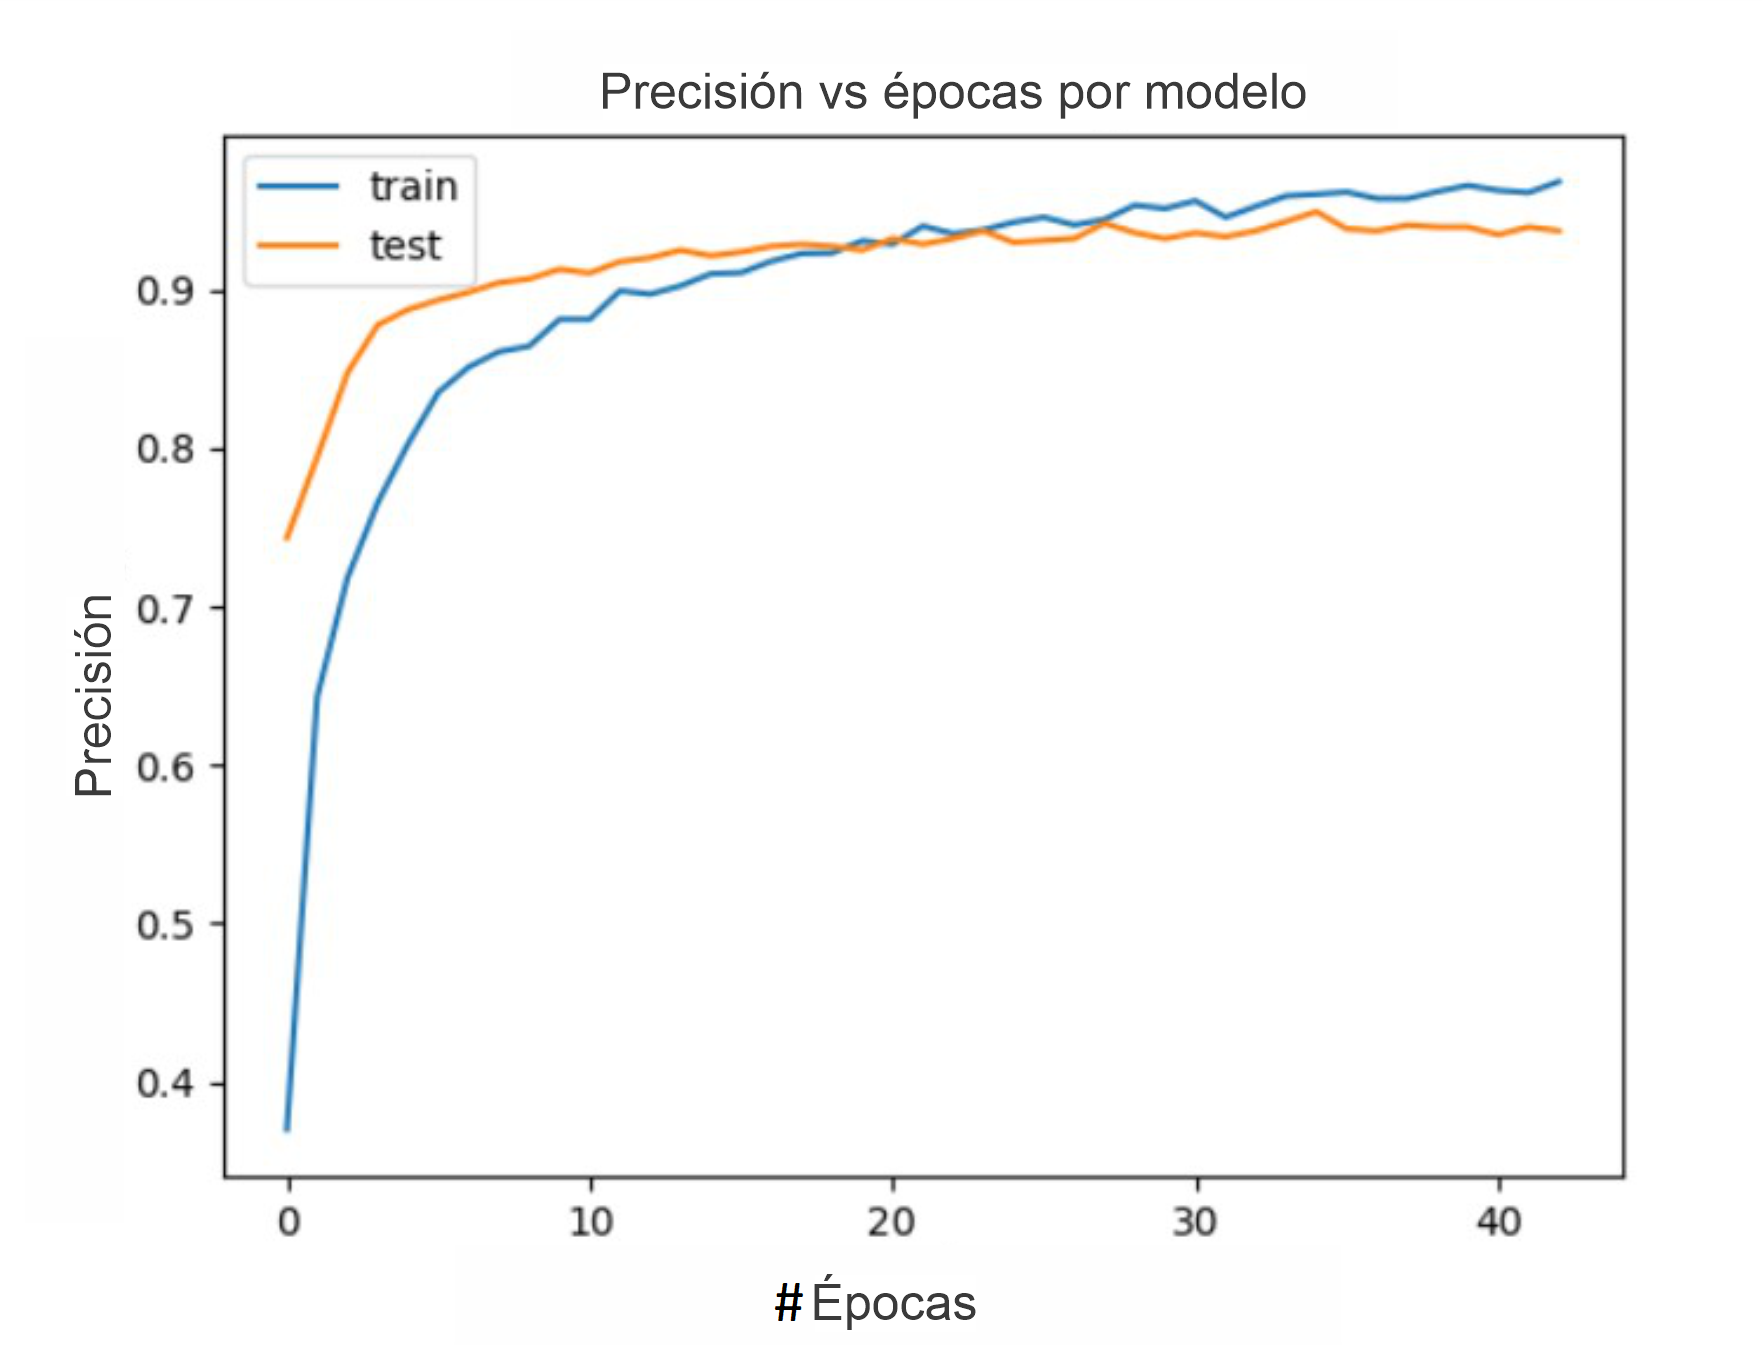
\includegraphics[width=0.8\textwidth]{images/accuracy4.png}
\caption{Gráfica comparativa de la precisión de entrenamiento y validacion}
\label{fig:accuracy4}
\end{figure}


Las gráficas muestran un aprendizaje constante, lo que refuerza la conclusión de que la red está aprendiendo correctamente, evitando aprender en exceso de ciertas clases e incluso obteniendo resultados positivos con las clases que tienen menor cantidad de imágenes. Además, es importante destacar que, en comparación con los experimentos previos del clasificador, estas nuevas redes podrían estar tardando más épocas en aprender de los datos debido a la complejidad de los mismos.

\subsection{Expermientación \#3 (extracción de datasets desde \textit{training}+\textit{testing})}
Con los resultados del anterior experimento se planteó unificar ambos \textit{datasets} y en base a esa nueva distribución de datos realizar la separación de los \textit{datasets }de \textit{training}, \textit{validation} y \textit{testing}. Dicha separación se realizó con los mismos porcentajes del anterior experimento. Al ejecutar la prueba, se obtuvieron los resultados de la tabla \ref{table:Results5}


\begin{table}[h!]
\centering
\begin{tabular}{|r|r|r|r|r|r|}
\hline
\textit{}           & \multicolumn{1}{c|}{\textit{Loss}} & {\textit{\begin{tabular}[c]{@{}c@{}}Balanced\\ Accuracy\end{tabular}}} & \multicolumn{1}{c|}{\textit{F1-weighted}} & \multicolumn{1}{c|}{\textit{Precision}} & \multicolumn{1}{c|}{\textit{Recall}} \\ \hline
\textit{Train}      & 0.2061                               & 93.04\%                                & 93.12 \%                          & 93.93\%                                 & 92.34\%                              \\ \hline
\textit{Validation} & 0.4659                               & 87.83\%                                & 88.11\%                          & 88.36\%                                 & 87.87\%                              \\ \hline
\textit{Testing}    & 0.4564                              & 87.73\%                                & 88.47\%                          & 90.06\%                                 & 88.03\%                              \\ \hline
\end{tabular}
\caption{Estadísticos otenidos del experimento \#3}
\label{table:Results5}
\end{table}


La unión de ambos \textit{datasets} ha arrojado resultados positivos, lo que confirma que sí había una gran diferencia en la distribución de los datos, lo que causaba que el modelo no genere una buena predicción al momento de realizar el \textit{testing}. Además, las gráficas de error y precisión (imágenes \ref{fig:losses5} y \ref{fig:accuracy5}) muestran el descenso en el error y el aumento en la precisión esperados.

\begin{figure}[h!]
\centering
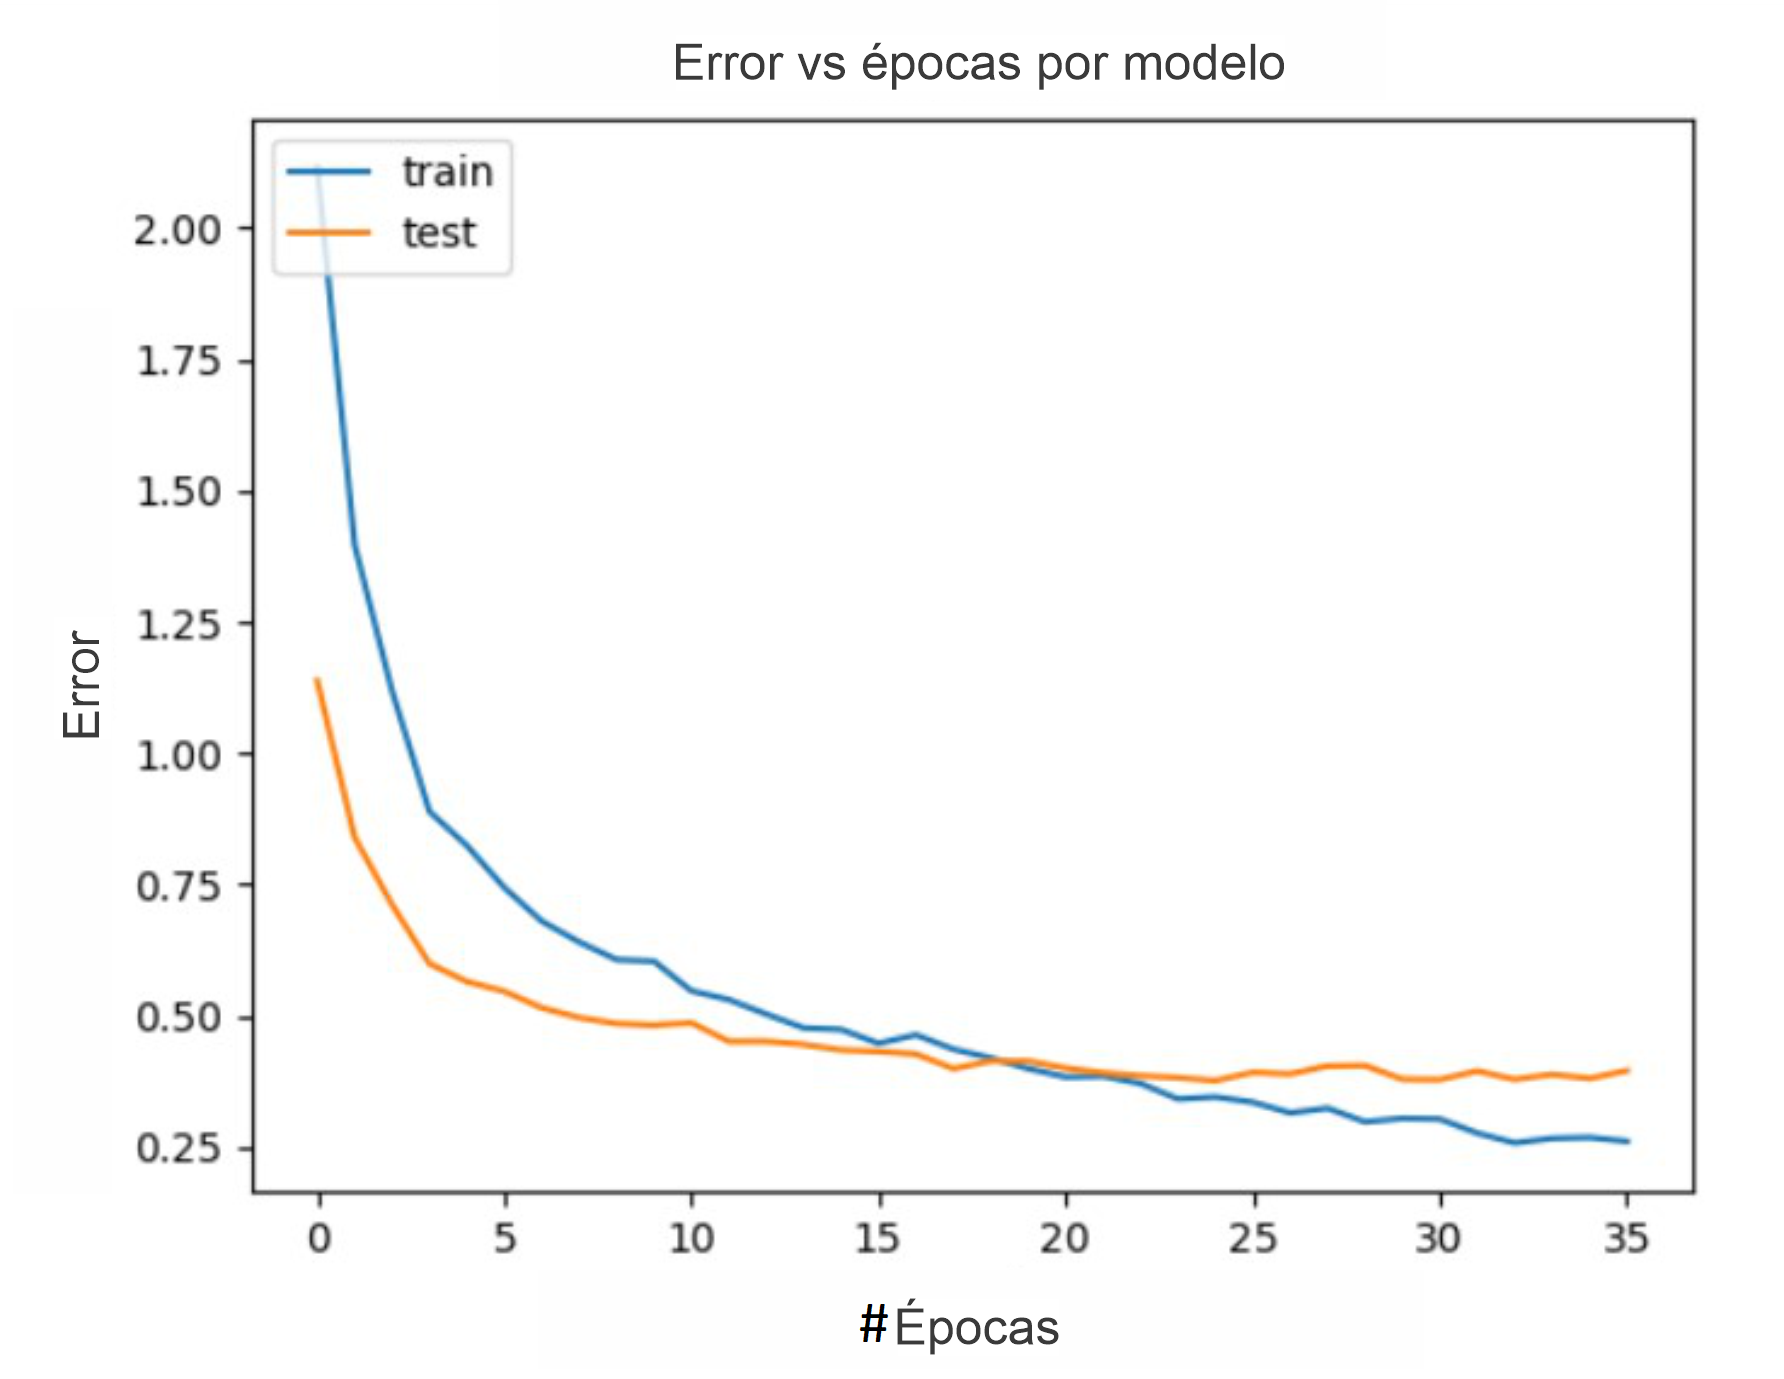
\includegraphics[width=0.8\textwidth]{images/loss5.png}
\caption{Gráfica comparativa de la perdida de entrenamiento y validacion del experimento \#3}
\label{fig:losses5}
\end{figure}

\begin{figure}[h!]
\centering
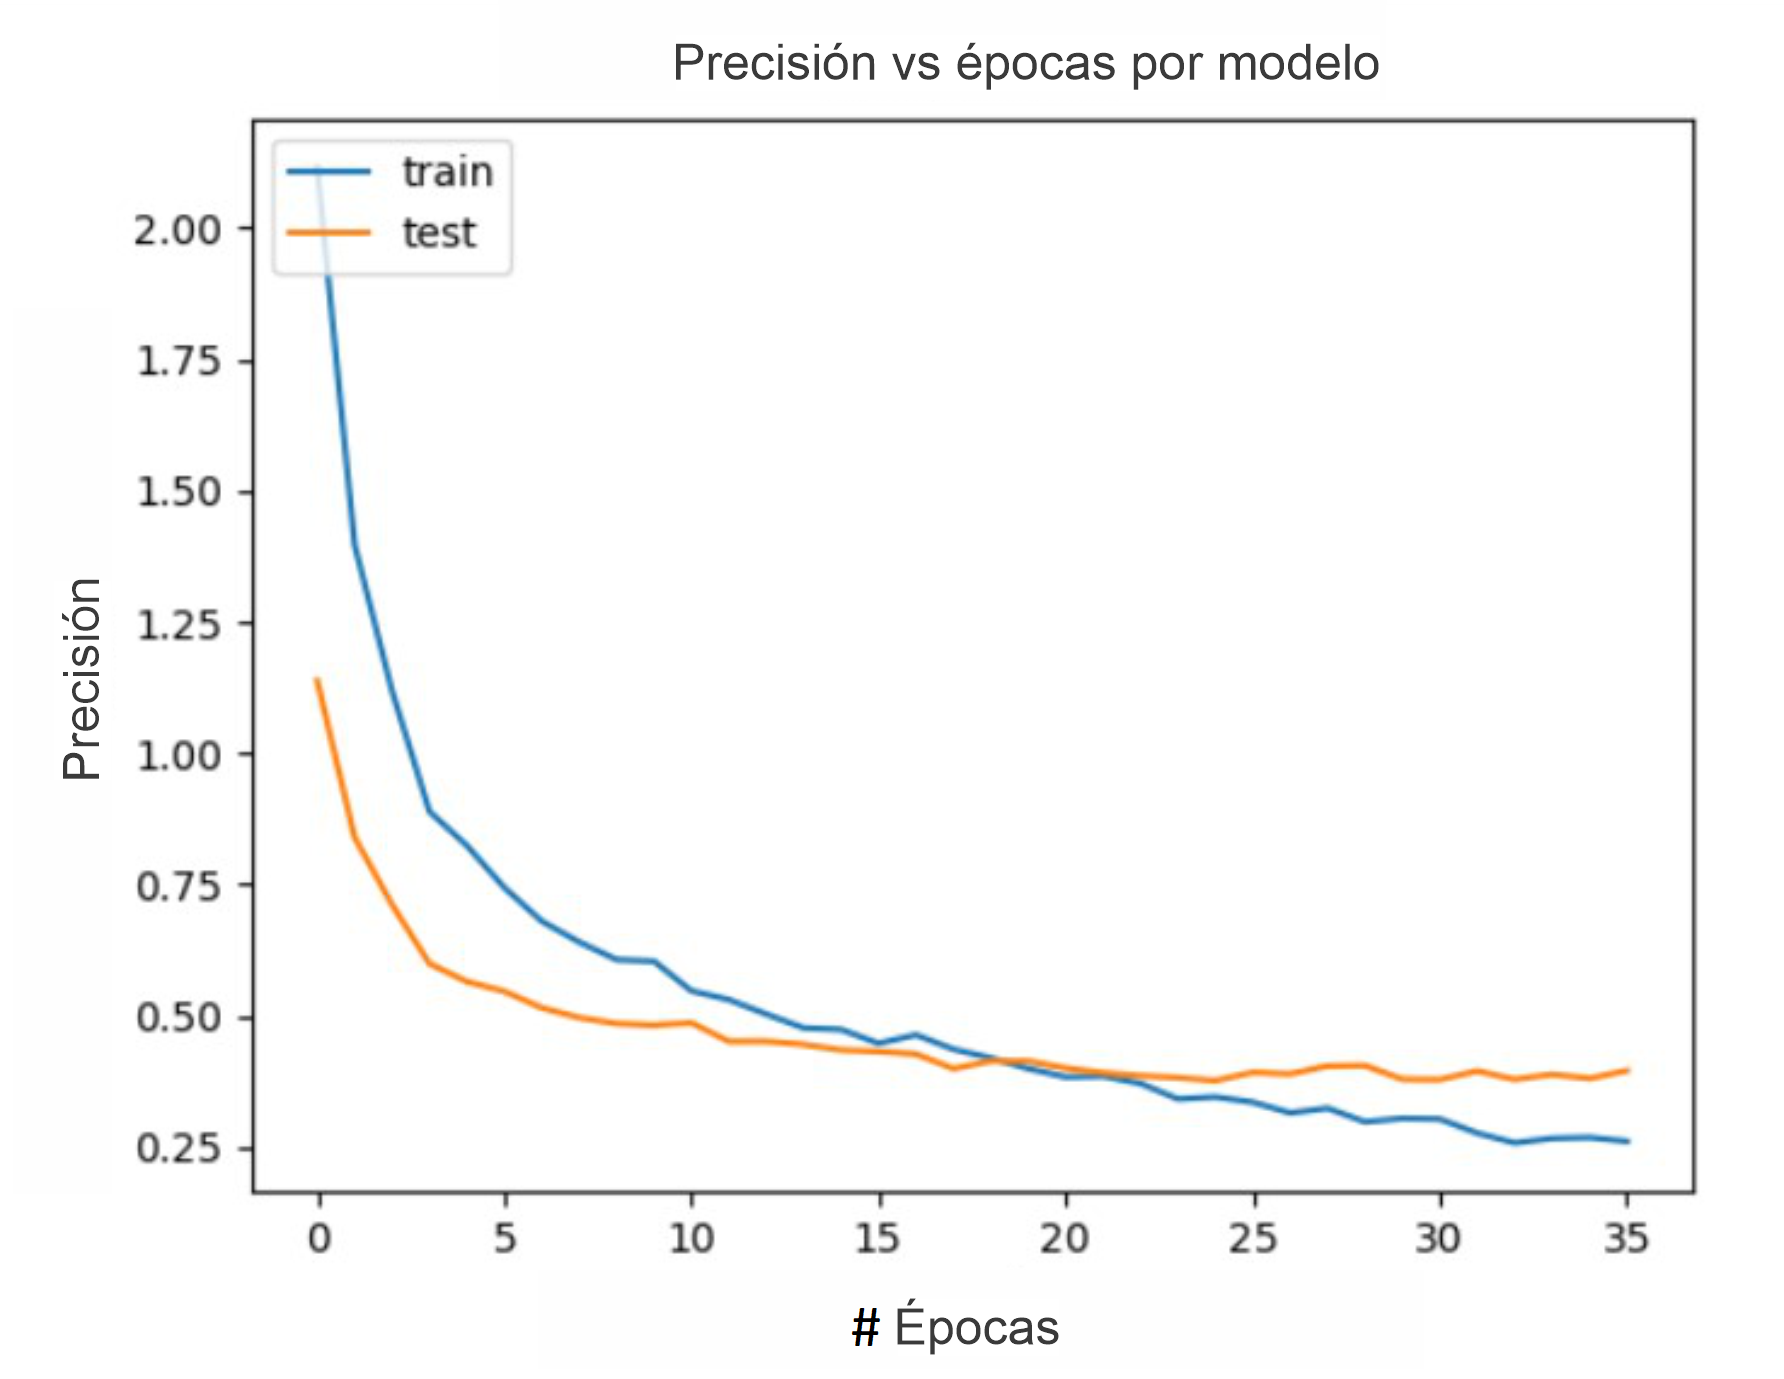
\includegraphics[width=0.8\textwidth]{images/accuracy5.png}
\caption{Gráfica comparativa de la precisión de entrenamiento y validacion del experimento \#3}
\label{fig:accuracy5}
\end{figure}

Por último, se realizó la matriz de confusión de las clases clasificadas que se pueden ver en la tabla \ref{fig:Matrix3}

\begin{figure}[h!]
\centering
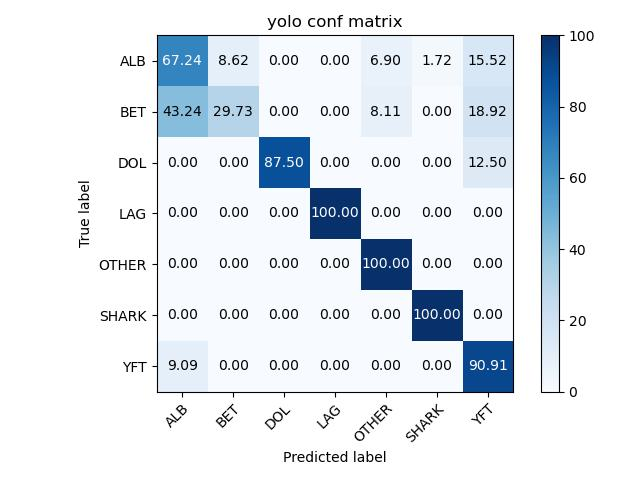
\includegraphics[width=0.8\textwidth]{images/yolo_conf_matrix.jpg}
\caption{Matriz de confusión generada por el experimento \#3 en porcentajes}
\label{fig:Matrix3}

\end{figure}

Con base en los resultados obtenidos, se puede afirmar que este modelo está preparado para ser utilizado en el \textit{pipeline} correspondiente. Es importante destacar que el entrenamiento de este modelo tardó 36 épocas, con un promedio de 10 segundos por época, lo que significa que el tiempo total de entrenamiento fue de 6 minutos, un tiempo relativamente corto. Además, el tiempo de procesamiento por \textit{batch} (32 imágenes) es de 85 ms, lo que indica que en el futuro se podría ampliar la base de datos con más imágenes de especies adicionales, para proporcionar una mayor especificidad en la detección de objetos o animales por medio del detector. En comparación, el proceso de entrenamiento para una red más compleja, que requiera una base de datos etiquetada, sería significativamente más largo y complicado.

\section{Experimentación del \textit{pipeline}}
Debido a que el \textit{pipeline} consta de dos pasos para la detección y clasificación de las imágenes, realizar una experimentación típica se hace inviable. En ese sentido, se simuló un \textit{benchmark} utilizando el flujo descrito por la imagen \ref{fig:metodologia2}

\begin{figure}[h!]
\centering
\includegraphics[width=0.9\textwidth]{images/Metodología2.png}
\caption{Flujo para la experimentación del \textit{pipeline}}
\label{fig:metodologia2}
\end{figure}

\subsection{Prueba del clasificador}

Una vez obtenidos las detecciones de los peces, quitado los errores del \textit{dataset} y etiquetar los peces que se tenían dentro del \textit{dataset} de prueba, se generaron tres nuevos \textit{datasets} de imágenes de peces detectados. Consiguientemente, se procedió a utilizar el modelo ya entrenado en la sección 5.4.3. 
A continuación se presentarán los resultados obtenidos para cada uno de los modelos, los cuales se recopilaron en la tabla \ref{table:estadisticosPipeline}.

\begin{table}[h!]
\footnotesize
\centering
\begin{tabular}{|c|c|c|c|c|}
\hline
                                                                                                                    & \textit{\begin{tabular}[c]{@{}c@{}}Balanced\\ Accuracy\end{tabular}} & \textit{F1-weighted} & \textit{\begin{tabular}[c]{@{}c@{}}Precision\\ weighted\end{tabular}} & \textit{\begin{tabular}[c]{@{}c@{}}Recall\\ weighted\end{tabular}} \\ \hline
\textit{\begin{tabular}[c]{@{}c@{}}Predicted Yolov5\\ pretrained(40\%\\ threshold)\end{tabular}}                    & 72.99\%                                                              & 68.35\%              & 76.08\%                                                               & 66.89\%                                                            \\ \hline
\textit{\begin{tabular}[c]{@{}c@{}}Predicted UniDet\\ pretrained (no \\ threshold)\end{tabular}}                    & 84.47\%                                                              & 84.67\%              & 86.50\%                                                               & 84.03\%                                                            \\ \hline
\textit{\begin{tabular}[c]{@{}c@{}}Predicted Yolov5\\ trained (freezed \\ backbone 95\% \\ threshold)\end{tabular}} & \textit{91.47\%}                                                              & \textit{91.90\%}              & \textit{91.99\%}                                                                & \textit{91.93\%}                                                            \\ \hline
\end{tabular}
\caption{Estadisticos generados por los 3 diferentes modelos}
\label{table:estadisticosPipeline}
\end{table}

Los resultados obtenidos muestran que el \textit{pipeline} funciona relativamente bien con todos los diferentes detectores, generando un \textit{balanced accuracy} bastante elevado. Por otra parte, se puede ver que los \textit{pipelines} que utilizaban los detectores preentrenados obtuvieron un resultado similar, aunque peor que el que usabe el detector entrenado. Esto es debido a que los \textit{bounding boxes} generados por el modelo entrenado coincidían con las imágenes recortadas con las que se entrenó el clasificador, mientras que UniDet generaba resultados aproximados. Por otra parte el Yolov5 preentrenado los generaba de manera muy justa, haciendo necesario que sean preprocesadas antes de ser ingresados al clasificador, por lo que también eran aproximados.
Además se obtuvieron las matrices de confusión (Tablas \ref{fig:confusionMatrix1}, \ref{fig:confusionMatrix2} y \ref{fig:confusionMatrix3}) de cada uno de los experimentos, los cuales se muestran a continuación:

\begin{figure}[h!]
\centering
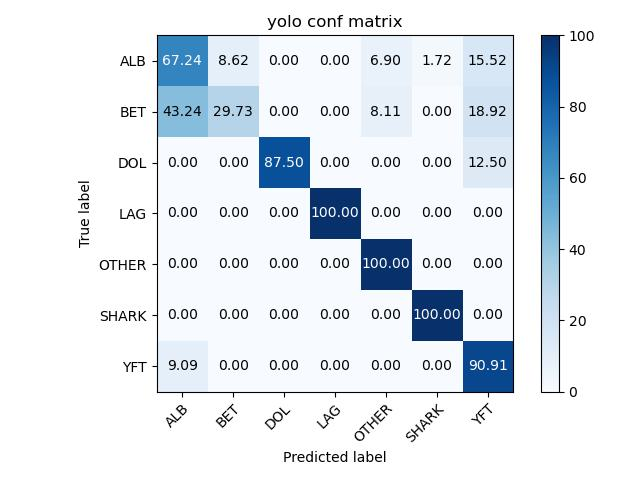
\includegraphics[width=0.8\textwidth]{images/yolo_conf_matrix.jpg}
\caption{Matriz de confusión para pruebas del \textit{pipeline} con Yolov5 preentrenado }
\label{fig:confusionMatrix1}
\end{figure}

\begin{figure}[h!]
\centering
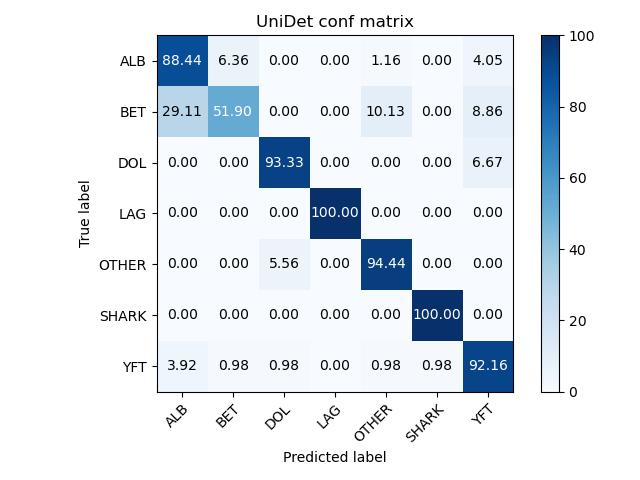
\includegraphics[width=0.8\textwidth]{images/UniDet_conf_matrix.jpg}
\caption{Matriz de confusión para el testeo del \textit{pipeline} con UnIDet preentrenado }
\label{fig:confusionMatrix2}
\end{figure}

\begin{figure}[h!]
\centering
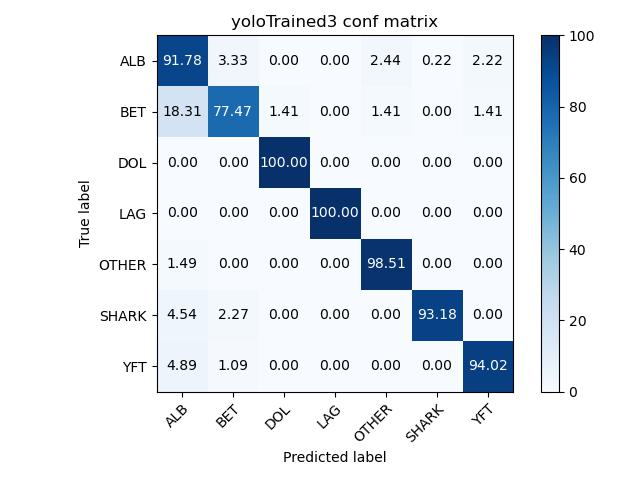
\includegraphics[width=0.8\textwidth]{images/yoloTrained3_conf_matrix.jpg}
\caption{Matriz de confusión para el testeo del \textit{pipeline} con Yolov5 entrenado }
\label{fig:confusionMatrix3}
\end{figure}
En general, se comprobó que el clasificador cumplió su función correctamente de clasificar las imágenes que le fueron proporcionadas por el detector. Aún así, la precisión de este radica en lo bien que fueron detectados los peces dentro de las imágenes. En ese sentido podemos ver que el aplicar este \textit{pipeline} generaría una pérdida en la precisión a comparación de entrenar un modelo de un 10\% a 28\% (que podría variar dependiendo del detector usado y del tratamiento de los \textit{bounding boxes}) en imágenes complejas como las que se tienen(sería conveniente realizar pruebas en imágenes menos complejas).

\section{Evaluación}

Finalmente, se comparó los resultados en términos de precisión final y el error generado de los modelos, tomando en cuenta la siguiente fórmula:
\newline
$$ precision\_final = \frac{peces\_detectados * accuracy\_clasificador}{imagenes\_reales}$$

Siguiendo esta métrica, y el porcentaje de error en la detección, se obtuvo la tabla de resultados final \ref{table:resultadosFinales}:
\begin{table}[h!]
\footnotesize
\begin{tabular}{|c|l|l|c|c|c|}
\hline
                                                                                                                    & \multicolumn{1}{c|}{\textit{\begin{tabular}[c]{@{}c@{}}Accuracy\\ parcial\end{tabular}}} & \multicolumn{1}{c|}{\textit{\begin{tabular}[c]{@{}c@{}}Accuracy \\ del \\ clasificador\end{tabular}}} & \textit{\begin{tabular}[c]{@{}c@{}}Accuracy\\ final\end{tabular}} & \textit{\begin{tabular}[c]{@{}c@{}}Porcentaje \\ de error\\ del total\end{tabular}} & \textit{\begin{tabular}[c]{@{}c@{}}Tiempo de \\ entrenamiento\end{tabular}}    \\ \hline
\textit{\begin{tabular}[c]{@{}c@{}}Predicted Yolov5\\ pretrained  (40\%\\ threshold)\end{tabular}}                  & \multicolumn{1}{c|}{14.13\%}                                                             & 72.99\%                                                                                          & 10.31\%                                                           & 69.07\%                                                                             & \begin{tabular}[c]{@{}c@{}}9 minutos\\ (CNN)\end{tabular}                      \\ \hline
\textit{\begin{tabular}[c]{@{}c@{}}Predicted UniDet\\ pretrained \\ (no threshold)\end{tabular}}                    & 40.15\%                                                                                  & 84.47\%                                                                                          & 33.91\%                                                           & \textbf{22.54\%}                                                                             & \begin{tabular}[c]{@{}c@{}}9 minutos\\ (CNN)\end{tabular}                      \\ \hline
\textit{\begin{tabular}[c]{@{}c@{}}Predicted Yolov5\\ trained  (backbone \\ freezed 95\%\\ threshold)\end{tabular}} & \textbf{79.45\%}                                                                                  & \textbf{91.47\%}                                                                                          & \textbf{72.67\%}                                                           & 32.36\%                                                                             & \begin{tabular}[c]{@{}c@{}}9 minutos(CNN) + \\ 80 minutos(yolov5)\end{tabular} \\ \hline
\end{tabular}
\caption{Accuracy final y porcentaje de errores detectados de los 3 modelos }
\label{table:resultadosFinales}
\end{table}

Considerando todos los experimentos realizados, podemos concluir que el \textit{pipeline} propuesto puede ser aplicable inclusive para casos complejos de manera que este no disminuye mucho el rendimiento de la precisión final ni aumenta mucho el tiempo de procesamiento. Además evita necesitar la obtención de un \textit{dataset} etiquetado con \textit{bounding boxes} para el entrenamiento, reducir el tiempo de entrenamiento y aumentar la escalabilidad de la especificación de especies detectadas. Cabe resaltar como punto importante que el desempeño de este \textit{pipeline} recae principalmente en poder encontrar un detector especializado o debidamente entrenado y robusto para poder detectar las diferentes clases y en el tratamiento de los \textit{bounding boxes} obtenidos para el paso por el clasificador. 
\chapter*{\center \Large CONCLUSIONES} 
\addcontentsline{toc}{section}{\bfseries CONCLUSIONES} 
\markboth{CONCLUSIONES}{CONCLUSIONES} 

En el presente trabajo se desarrolló un \textit{pipeline} para el
etiquetado de imágenes de peces peruanos, empleando técnicas de detección y 
clasificación en un entorno real. Para ello, se recolectó un 
\textit{dataset} de 5 mil imágenes aproximadamente a través de la plataforma 
Kaggle, conteniendo varios peces dentro de cada imagen, el cual fue 
recortado y clasificado por un experto. 
A través de la experimentación, se comprobó que un modelo 
ligero pero al mismo tiempo robusto como lo es EfficientNetB0 obtuvo una 
precisión similar (entre 76\% y 92\%) al ser usado con diferentes detectores 
dentro del \textit{pipeline}. 
De parte del detector, se pudo comprobar que un modelo entrenado (como lo es YoloV5) 
logra una mejor precisión inclusive comparándolo con una arquitectura más compleja 
(como lo es UniDet), teniendo una diferencia de 79.5\% y 40.15\%. Por el contrario, 
se obtuvo un menor error en la detección hecha por Unidet en general, siendo esta de 
22.54\%. 
\newline
\newline
Considerando los resultados obtenidos podemos afirmar que el performance y 
la precisión del \textit{pipeline} dependerá del modelo preentrenado para el detector, 
ya que el clasificador logrará clasificar correctamente (en su mayoría de veces) para lo 
que fue entrenado. En base a ellos, se logró desarrollar una aplicación en tiempo real, 
el cual permitió automatizar el proceso de etiquetado para imágenes y videos.

Cabe recalcar que la intención de este \textit{pipeline} no es reemplazar o mejorar al 
sistema basado únicamente en YOLO, sino ser un sustituto real en casos en donde 
se tenga un \textit{dataset} sin etiquetar y se quiera generar una solución a un 
problema de localización y clasificación de objetos. 



\chapter*{\center \Large RECOMENDACIONES} 
\addcontentsline{toc}{section}{\bfseries RECOMENDACIONES} 
\markboth{RECOMENDACIONES}{RECOMENDACIONES} 

Algunas de las limitaciones que se tiene con este modelo consisten en que el 
\textit{pipeline} depende casi completamente del detector escogido, de tal 
manera que se necesita poder obtener uno bastante robusto y entrenado de 
manera general o incluso mejor si está especialmente entrenado para detectar 
las clases que se están estudiando. De esta manera, se generarían buenas 
entradas para el clasificador, reduciendo el efecto que este tendría en el 
\textit{pipeline} final. En ese sentido, sería bueno poder realizar más 
experimentos con diferentes arquitecturas y modelos preentrenados que incluya 
la clase peces.
\\\\
De la misma manera, actualmente existen ciertos \textit{datasets} que son 
ampliamente utilizados para la investigación y creación de aplicaciones de 
DL, mientras que otros presentan pocas implementaciones, lo que hace más 
complicado la obtención de modelos preentrenados con las clases genéricas 
requeridas (por ejemplo, peces). En ese sentido, otro trabajo futuro 
consistiría en poder utilizar este etiquetador para crear un \textit{dataset} 
con la clase genérica de peces e incrementar una capa de atención a los modelos 
para poder analizar como se comporta el \textit{pipeline} con respecto al 
\textit{accuracy} parcial y final.   
\\\\
Por último, este trabajo se realizó con un \textit{dataset} de peces peruanos 
(en su mayoría) pero consistía de un bajo número de imágenes y consistían de 
una distribución de datos muy complejas. En ese sentido, el error y la 
precisión obtenidos también contemplaban \textit{bias} debido a estos factores. 
Es por ello que se recomendaría replicar las experimentaciones realizadas en 
el presente documento pero con un \textit{dataset} que incluya un número de 
especies e imágenes mayor para poder calcular como es que esto influye en la 
precisión, el costo de entrenamiento y si se necesita mejorar o incrementar 
algunas capas del modelo.
 % sección opcional
\chapter*{\center \Large ANEXOS} 
\addcontentsline{toc}{section}{\bfseries ANEXOS} 
\markboth{ANEXOS}{ANEXOS} 

\label{appendix}
Los siguientes experimentos fueron realizados para poder comprobar 
que la distribución de datos tanto del \textit{dataset} de 
entrenamiento como el de \textit{testing} eran diferentes, 
generando un \textit{overfitting} accidental en la experimentación 
general. 

\section{Experimentación A (training/ validation/ testing)}

Una vez de terminado la creación de los \textit{bounding boxes} de parte 
del experto, se procedió a realizar la comprobación del modelo en base a 
los datos de \textit{testing}. Los estadísticos resultantes del \textit{testing} 
fueron los mostrados en la tabla \ref{table:Anexo2}.
\begin{table}[h!]
\centering
\begin{tabular}{|l|l|l|l|l|}
\hline
\multicolumn{1}{|c|}{\textit{Loss}} & \textit{\begin{tabular}[c]{@{}c@{}}Balanced\\Accuracy\end{tabular}}  & \multicolumn{1}{c|}{\textit{F1-weighted}} & \multicolumn{1}{c|}{\textit{Precision}} & \multicolumn{1}{c|}{\textit{Recall}} \\ \hline
2.7014          & 46.50\%                          & 41.46\%                  & 50.28\%                         & 49.54\%                      \\ \hline
\end{tabular}
\caption{Estadísticos obtenidos del experimento \#A}
\label{table:Anexo2}
\end{table}

Los estadísticos obtenidos empeoraron en comparación con los datos de 
entrenamiento. Para confirmar las sospechas de un posible 
\textit{overfitting}, se revisaron las gráficas de pérdida a través de 
las épocas, que se pueden ver en la imagen \ref{fig:losses3}.

\begin{figure}[h!]
\footnotesize
\centering
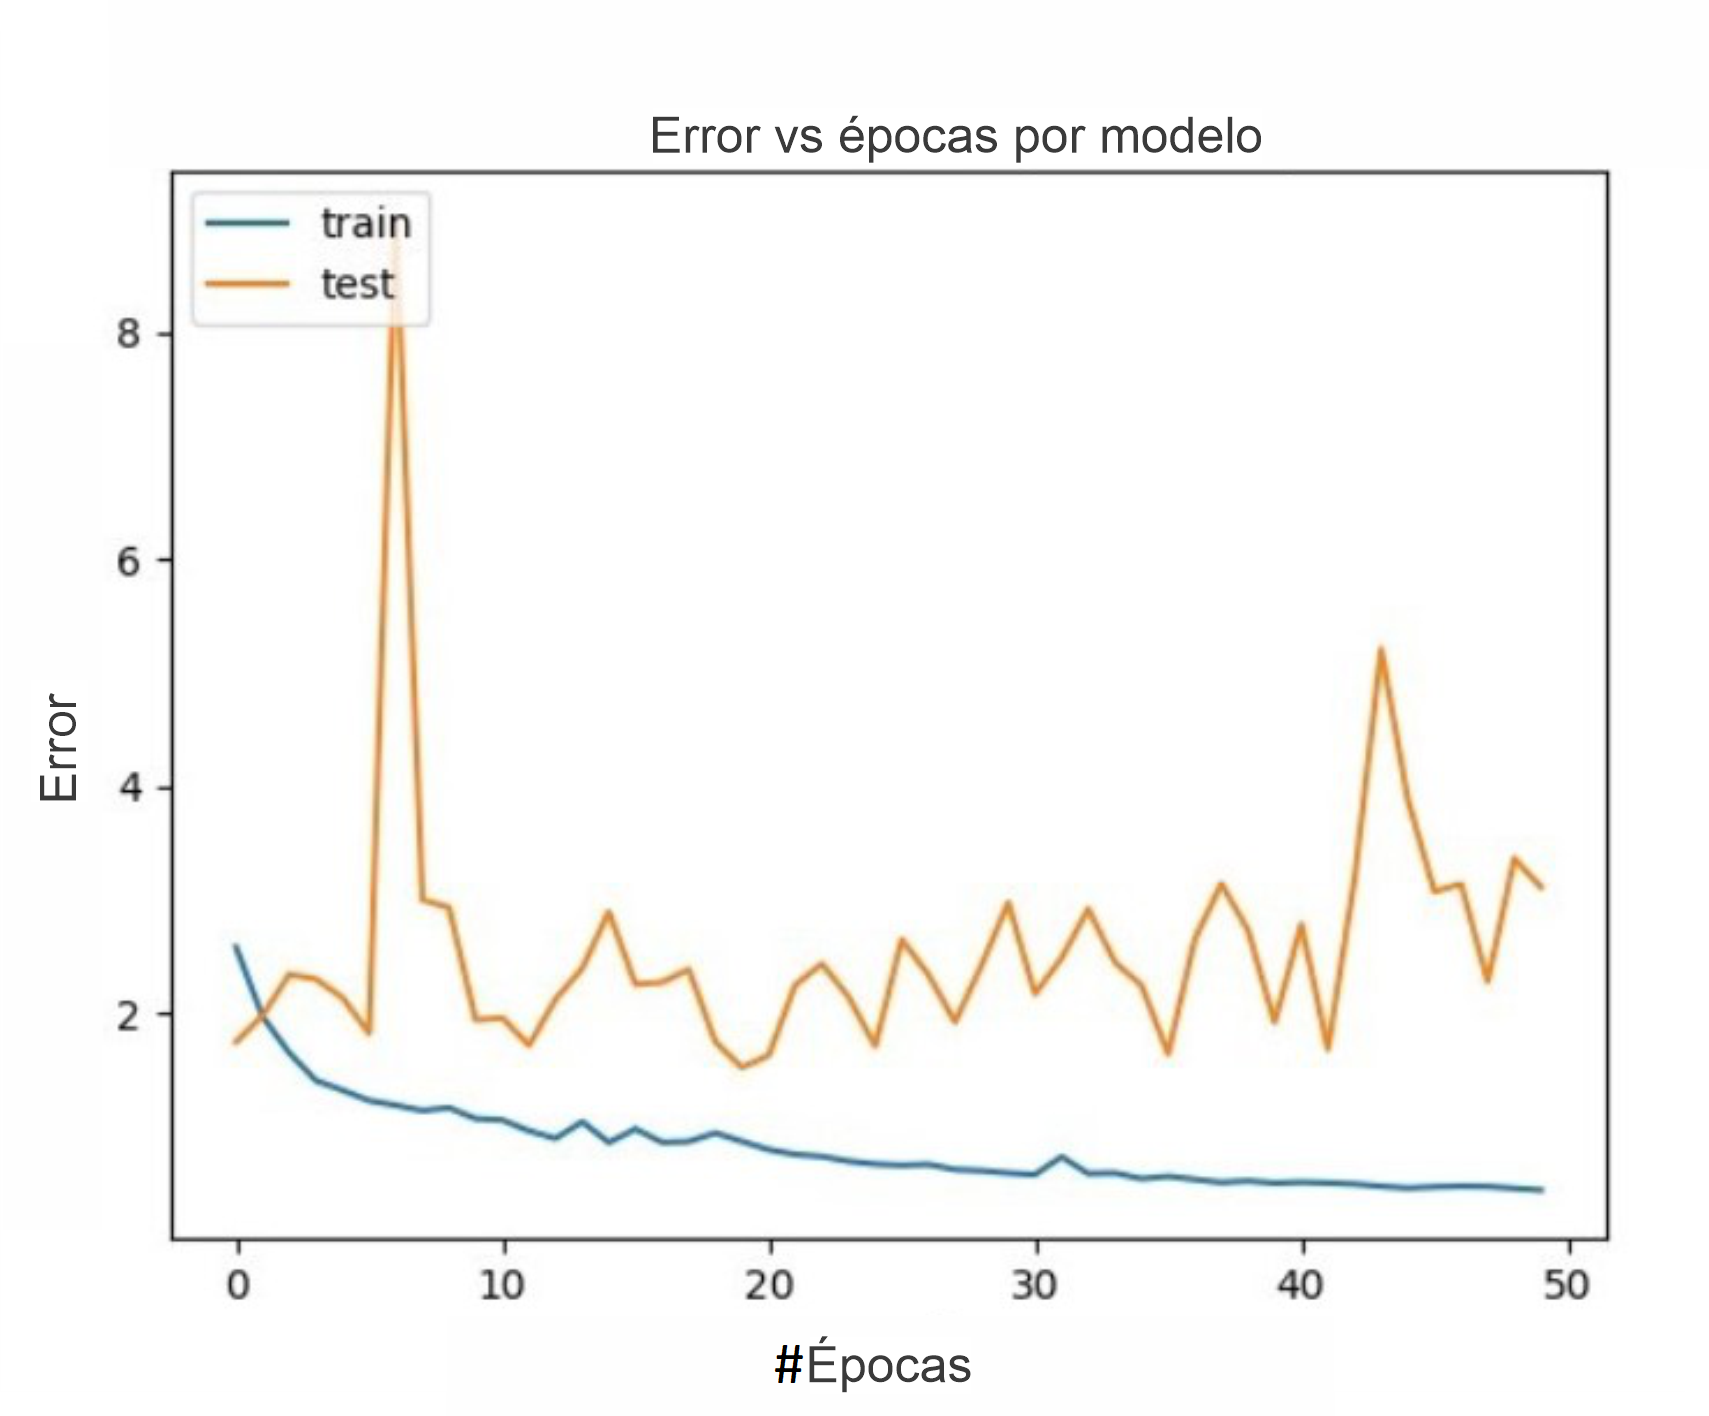
\includegraphics[width=1\textwidth]{images/loss3.png}
\caption{Gráfica comparativa de la perdida de entrenamiento y \textit{testing}}
\label{fig:losses3}
\end{figure}

Una vez más, la gráfica muestra un posible caso de \textit{overfitting} de los 
datos y, aún peor, la gráfica de error indica un aumento en lugar de una disminución 
a lo largo de las épocas. Para evaluar de manera más detallada los resultados, 
se revisó la matriz de confusión generada, la cual se muestra en la tabla 
\ref{table:Matrix1}.
\newpage
\begin{table}[h!]
\footnotesize
\begin{tabular}{|c|c|c|c|c|c|c|c|}
\hline
                                                                  & \begin{tabular}[c]{@{}c@{}}Albacore\\ Tuna\end{tabular} & \begin{tabular}[c]{@{}c@{}}Bigeye\\ Tuna\end{tabular} & \begin{tabular}[c]{@{}c@{}}Dolphin\\Fish\end{tabular} & \begin{tabular}[c]{@{}c@{}}Moonfish\\ (LAG)\end{tabular} & Shark   & \begin{tabular}[c]{@{}c@{}}Yellowfin\\ Tuna\end{tabular} & Other   \\ \hline
\textit{\begin{tabular}[c]{@{}c@{}}Albacore\\ Tuna\end{tabular}}  & 94.26\%                                                 & 00.78\%                                               & 00.00\%     & 00.00\%                                                  & 00.78\% & 01.57\%                                                  & 02.61\% \\ \hline
\textit{\begin{tabular}[c]{@{}c@{}}Bigeye\\ Tuna\end{tabular}}    & 88.23\%                                                 & 03.07\%                                               & 00.00\%     & 00.00\%                                                  & 00.51\% & 00.77\%                                                  & 07.42\% \\ \hline
\begin{tabular}[c]{@{}c@{}}Dolphin\\Fish\end{tabular}                                              & 35.00\%                                                 & 00.00\%                                               & 50.00\%     & 00.00\%                                                  & 00.00\% & 05.00\%                                                  & 10.00\% \\ \hline
\textit{\begin{tabular}[c]{@{}c@{}}Moonfish\\ (LAG)\end{tabular}} & 25.42\%                                                 & 00.00\%                                               & 03.39\%     & 57.63\%                                                  & 06.78\% & 00.00\%                                                  & 06.78\% \\ \hline
\textit{Shark}                                                    & 50.38\%                                                 & 00.76\%                                               & 00.00\%     & 00.00\%                                                  & 38.93\% & 04.58\%                                                  & 05.34\% \\ \hline
\textit{\begin{tabular}[c]{@{}c@{}}Yellowfin\\ Tuna\end{tabular}} & 33.33\%                                                 & 09.52\%                                               & 00.00\%     & 00.00\%                                                  & 00.00\% & 38.09\%                                                  & 19.05\% \\ \hline
\textit{Other}                                                    & 23.78\%                                                 & 01.22\%                                               & 01.22\%     & 00.00\%                                                  & 00.00\% & 00.00\%                                                  & 73.78\% \\ \hline
\end{tabular}
\caption{Matriz de confusión generada por las imágenes de \textit{testing} en porcentajes}
\label{table:Matrix1}
\end{table}


En la tabla se puede observar que la red tiende a predecir que los ejemplares 
pertenecen a la primera especie, lo que sugiere que está sobre aprendiendo de esta 
clase, posiblemente debido a la mayor cantidad de datos disponibles. A pesar de que 
esta hipótesis podría parecer plausible, no es la correcta, como se verá en los siguientes experimentos.

\section{Experimentación B (training/ validation/ testing con \textit{unfreeze})}

Para intentar reducir el posible \textit{overfitting}, se decidió quitar el 
\textit{freeze} de los dos últimos bloques de capas convolucionales del modelo pre-entrenado, 
permitiendo así que el modelo aprenda más patrones dentro de las imágenes. Después de esta 
modificación, se obtuvieron los resultados que se muestran en la tabla \ref{table:Results3}.

\begin{table}[h!]
\centering
\begin{tabular}{|l|l|l|l|l|l|}
\hline
                                                                            & \multicolumn{1}{c|}{\textit{Loss}} & \textit{\begin{tabular}[c]{@{}c@{}}Balanced\\Accuracy\end{tabular}} & \multicolumn{1}{c|}{\textit{F1-weighted}} & \multicolumn{1}{c|}{\textit{Precision}} &  \multicolumn{1}{c|}{\textit{Recall}} \\ \hline
\textit{\begin{tabular}[c]{@{}l@{}}Bloque 7 \\ unfreezed\end{tabular}}      & 4.1616                              & 51.71\%                                 & 42.23\%                           & 51.17\%                                  & 50.92\%                               \\ \hline
\textit{\begin{tabular}[c]{@{}l@{}}Bloques 6 y 7 \\ unfreezed\end{tabular}} & 3.1206                              & 19.56\%                                 & 28.97\%                           & 40.58\%                                  & 33.90\%                               \\ \hline
\end{tabular}
\caption{Estadísticos obtenidos del experimento \#3}
\label{table:Results3}
\end{table}

De la misma manera, las gráficas de error y \textit{accuracy}, junto con las matrices de 
confusión resultaron similares al anterior experimento, por lo que surgió la duda acerca 
de si tal vez existía una incongruencia con la base de datos.
% sección opcional


%% ============================================================================
\renewcommand{\bibname}{\large\bf{REFERENCIAS BIBLIOGR\'AFICAS}}
\bibliographystyle{IEEEtran} % Use the IEEEtran style
\bibliography{referencias}   % The references are in "referencias.bib"

\end{document}
%% ----------------------------------------------------------------


%%% Local Variables:
%%% mode: latex
%%% TeX-master: t
%%% End:
